From all these Starcraft 2 match results, one possible data product that crossed our mind was a predictor that could predict the victor of a match given the players involved and the map they are playing. With this goal in mind, we proceeded as follows. 

\subsection{Models}
To tackle this problem, we approached it as a classification problem. More specifically, we could train a classifier model on a player's past matches, then feed it upcoming match data. The output would simply be a binary classification (i.e. \textbf{lose} or \textbf{win}). Through the miracles of scikit-learn, we were able to experiment with the following models:

\begin{enumerate}
\item Logistic Regression
\item Decision Trees
\item Multinomial Bayes
\item Support Vector Machine
\item Random Forests
\item Stacking Ensembles
\begin{enumerate}
\item Logistic Regression
\item Multi-Response Linear Models
\end{enumerate}
\end{enumerate}

For more information on these models, it is sufficient to either Google or Wikipedia for the terms.

\subsection{Features}
Before tinkering with the models, we put a bit of thought on what features would characterize a player's performance. Though there are some established metrics, particularly the infamous APM, we discounted this on the basis that on the professional stage, the level of game mechanics is on an equal level among the players. Instead, the decisions that a player makes against his or her opponent is the biggest factor on victory. At this high level, the strategies one chooses is dependent on two things: the opponent's race and the map being played. Keeping this in mind, we began with the following features:

\begin{enumerate}
\item \textbf{player's win rate against opponent's race on map} - For a professional player, they tend to usually select a specific strategic based on which map they are on and what race they are playing against. This metric seems to capture the player's accuracy in selecting a successful strategy.
\item \textbf{opponent's win rate against player's race on map} - For the same reasons above, we included this for the opponent.
\item \textbf{player's win rate against opponent overall} - Considering how players tend to study their opponents tactics, this metric seems to capture how accurately a player can read their opponent.
\item \textbf{time} - It made sense to factor in time to account for Starcraft 2's constantly changing metagame due to patches and evolving plays.
\end{enumerate}

The results for these features can be seen in \ref{sec:evaluation1}. With some thought, we stumbled on these additional features:

\begin{enumerate}
\setcounter{enumi}{4}
\item \textbf{player's win rate on map} - After some consideration, it hit upon us that players also tend to take advantage of some features of a map on the fly during a match, which is potentially modeled in this feature.
\item \textbf{opponent's win rate on map} - For the same reasons above, we included this for the opponent.
\item \textbf{player's win rate against opponent's race} - With further thinking, we also realized that players are not limited to using specific strategies for a race based on a map. To factor this in, we felt that this feature was the closest indicator of the success of a player's strategy.
\item \textbf{opponent's win rate against player's race} - For the same reasons above, we included this for the opponent.
\end{enumerate}

The results for these features can be seen in \ref{sec:evaluation2}. Yet, with some more thoughts, we figured out one additional feature:

\begin{enumerate}
\setcounter{enumi}{8}
\item \textbf{player's win rate against opponent on map} - Keeping in mind how players have an intuitive idea of what tricks their opponents may try on a specific map, this feature seemed to be the best choice for representing this intuition.
\end{enumerate}

\subsection{Evaluation of Models}
\label{sec:evaluation}
As noted in the above sections, we evaluated each model we had on multiple feature sets. To do these evaluations, we ran a 10-fold cross validation on each model with the given features, plotted ROC curves for each fold, then examined the average ROC curve. For the actual player, we settled on using MVP, a well known Terran player with an average amount of matches.

\subsubsection{Features 1-4}
\label{sec:evaluation1}
Refer to Figure \ref{fig:fig1} for the results. From a quick inspection at the overall AUC average, the feature selection seems to be pretty good. However, considering the variance in the ROC curves for a majority of the models, it seems as if any of these models will not have consistent performance. From comparing the models, it's clear that the stacking MLR model is the best.

\subsubsection{Features 1-8}
\label{sec:evaluation2}
Refer to Figure \ref{fig:fig2} for the results. Compared to the results in \ref{sec:evaluation1}, the changes are very minimal, which seems to imply that a few of the included features are redundant. In addition, these results indicate stacking MLR is once again the best choice.

\subsubsection{Features 1-9}
\label{sec:evaluation3}
Refer to Figure \ref{fig:fig3} for the results. Interestingly, including the player's win rate heavily improves the performance of all the models. However, as we point out in \ref{sec:selection}, this is actually an issue of leaking, or overfitting the data set. Yet, even though all the models are performing at a similar level, the stacking MLR is still the best choice overall.

\subsection{Selection of Models and Features}
\label{sec:selection}

From looking at the evaluations in \ref{sec:evaluation}, the most obvious choice in features would be using all the features. However, this is actually the worst one to use because any of the models overfits. Why is this the case? In a roundabout way, our models are actually trying to predict the win rate of the player against the opponent on that specific map. Clearly, if we give the model this value as a feature, it's simply going to fit only on that as a feature. As a result, it overfits and yields lopsided values. With this in mind, it was clear that the best choice would then be features used in \ref{sec:evaluation2}, as these were the next best without overfitting. Finally, since stacking MLR was consistently the best performer, we chose this as our model.

\subsection{Model Predictions}
To test drive our model, we decided to predict the outcome of recent matches played in the GSL Code S League. The results are as follows:

NOTE: Percentages indicate player's chance of winning according to the model. Ties in classification are broken by which model's confidence is higher.

\begin{center}
\begin{tabular}{| l | l | l | l | l | l | l | l |}
\hline
Map & P1 & P2 & P1's \% & P2's \% & Prediction & Actual \\
\hline
Cloud Kingdom & Parting & TheStC & 93\% & 3\% & Parting & Parting \\
Antiga Shipyard & Parting & TheStC & 82\% & 1\% & Parting & Parting \\
Atlantis Spaceship & MarineKing & TaeJa & 12\% & 83\% & TaeJa & MarineKing \\
Cloud Kingdom & MarineKing & TaeJa & 3\% & 95\% & TaeJa & MarineKing \\
Metropolis & Parting & MarineKing & 35\% & 95\% & MarineKing & Parting \\
Entombed Valley & Parting & MarineKing & 1\% & 98\% & MarineKing & MarineKing \\
Daybreak & Parting & MarineKing & 25\% & 25\% & MarineKing & Parting \\
Metropolis & TheStC & TaeJa & 94\% & 1\% & TheStC & TaeJa \\
Daybreak & TheStC & TaeJa & 94\% & 5\% & TheStC & TaeJa \\
Entombed Valley & TaeJa & MarineKing & 13\% & 40\% & MarineKing & TaeJa \\
Dual Sight & TaeJa & MarineKing & 31\% & 14\% & TaeJa & TaeJa \\
\hline
\end{tabular}
\end{center}

From the above, there is something our model is lacking since it is only capable of predicting 4 out of 11 matches correctly - or in other words, it does worse then random guessing. It's clear that this is a good example of how simple validation is not always enough to guarantee actual success on new data.

\begin{figure}[t]
\centering
\subfloat[Logistic Regression]{
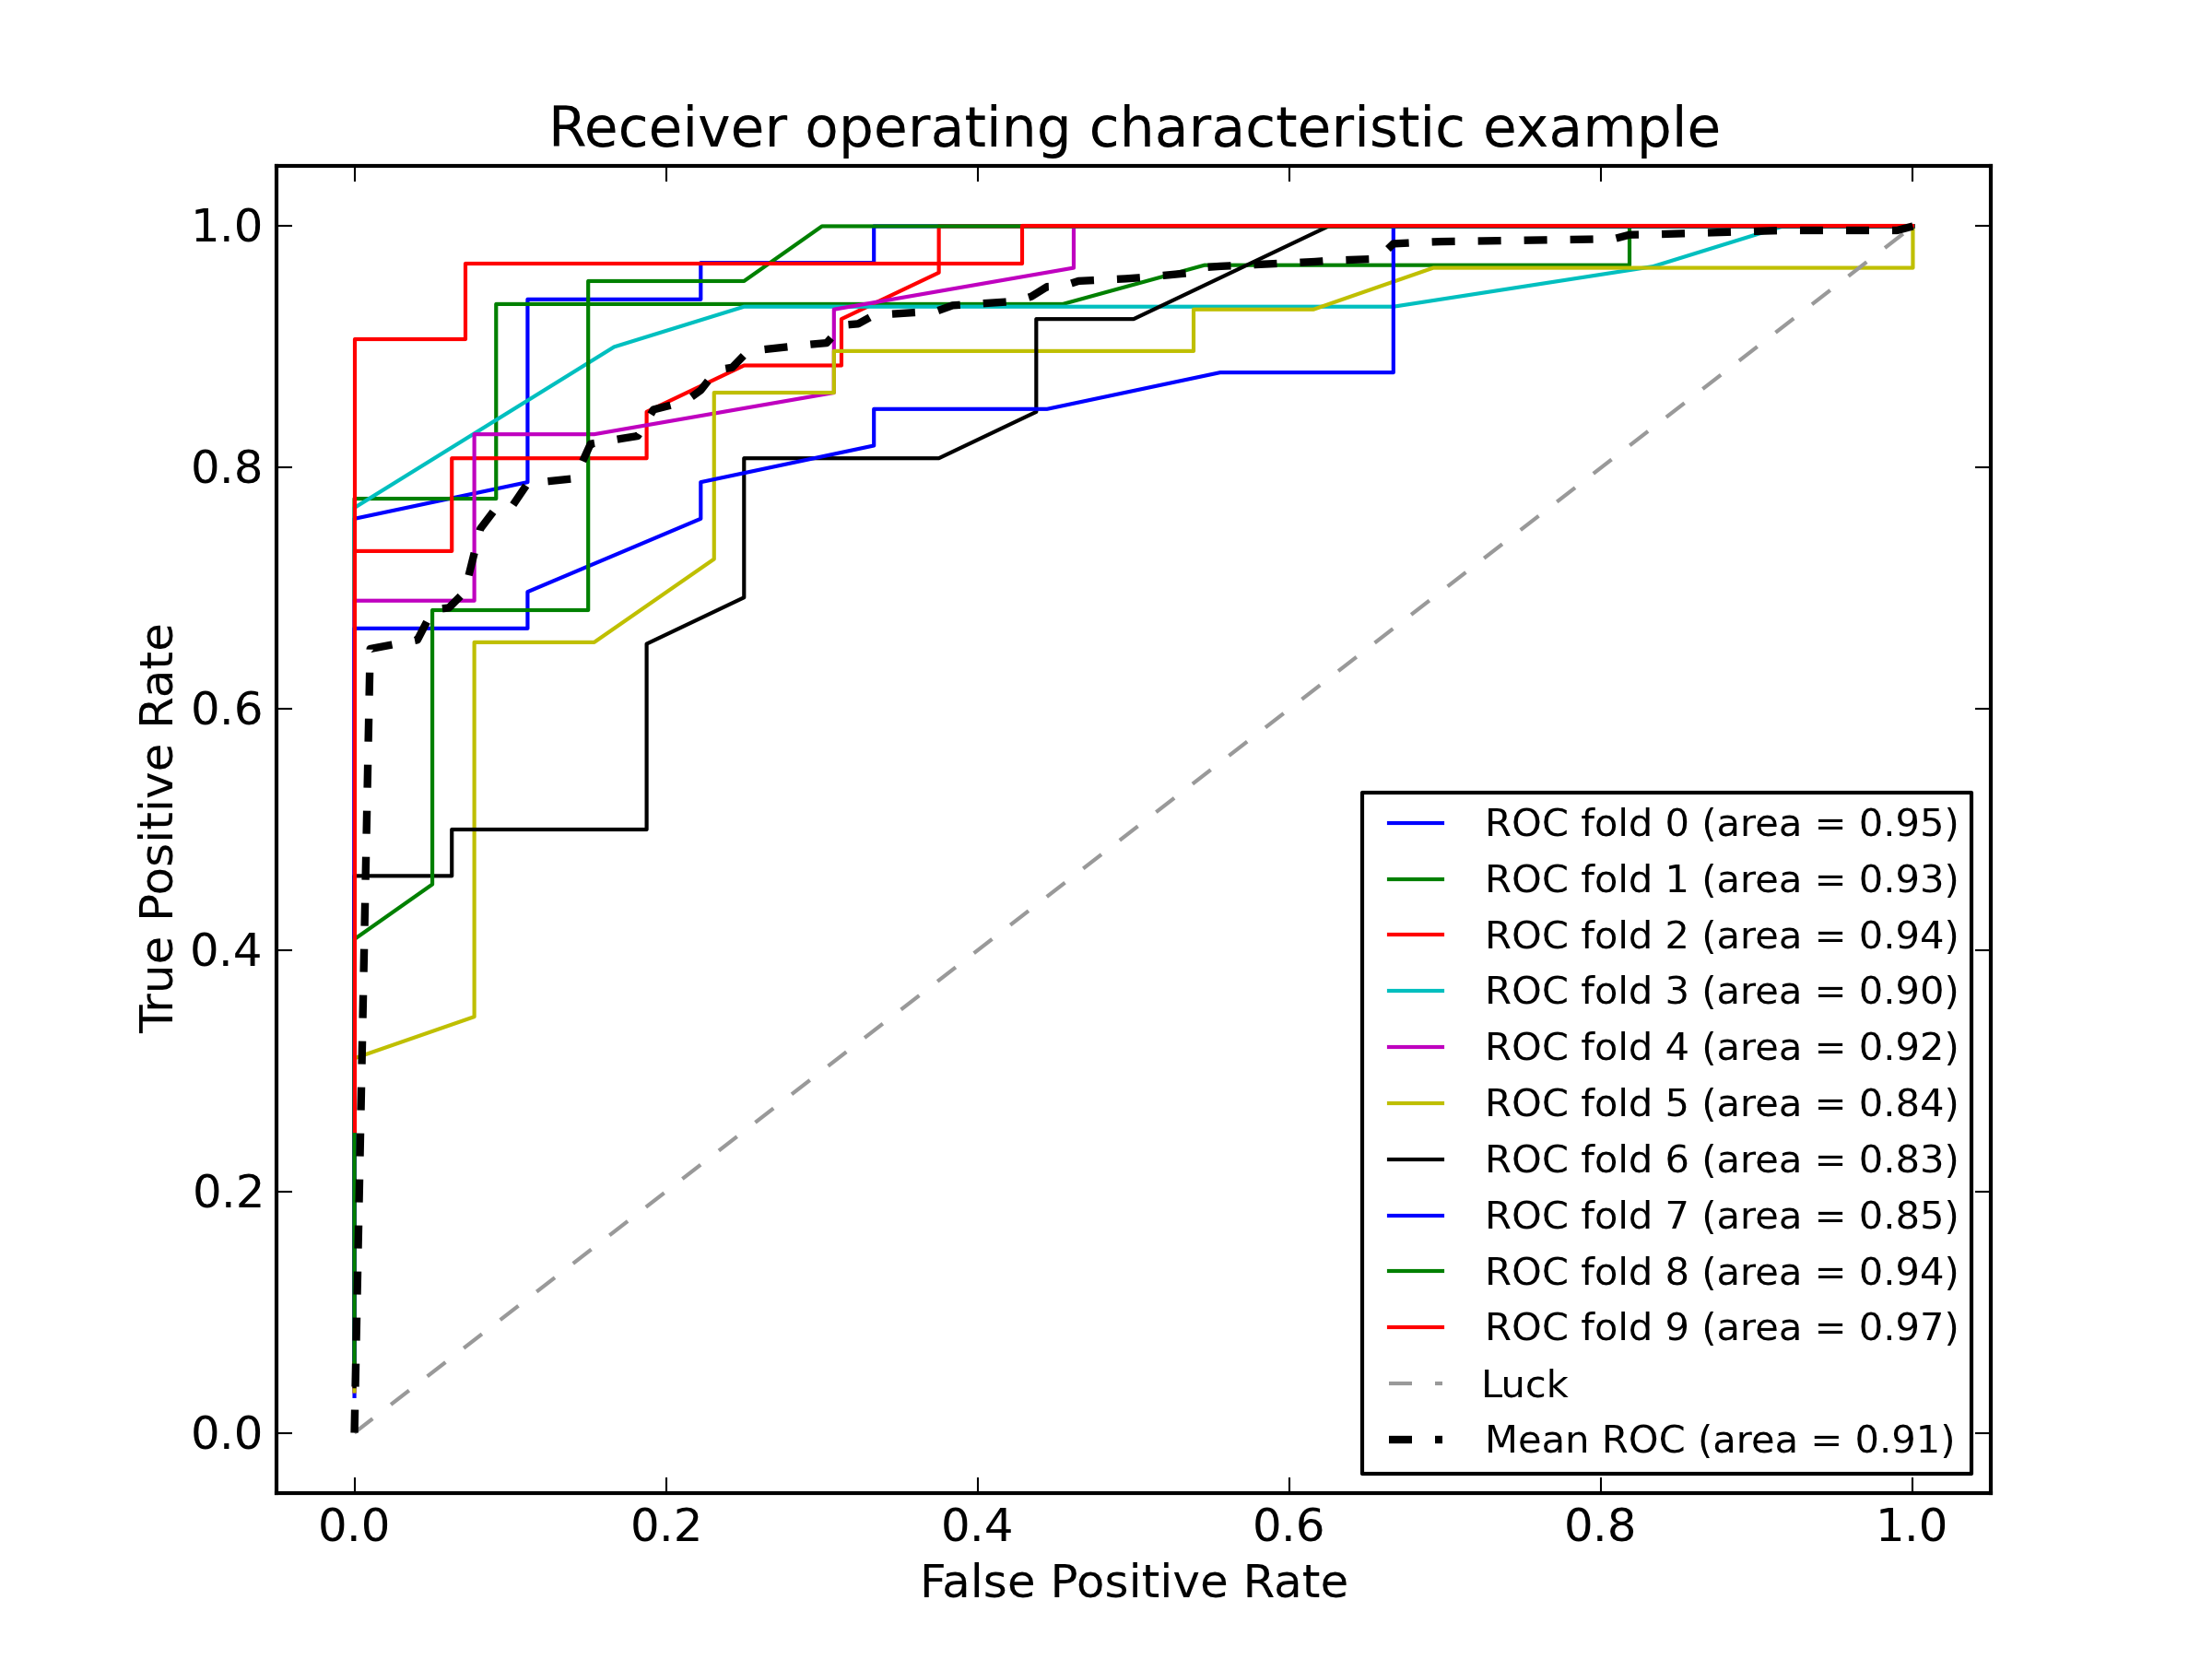
\includegraphics[width=0.36\textwidth]{pics/0_590_logit.png}}
\quad
\subfloat[Decision Trees]{
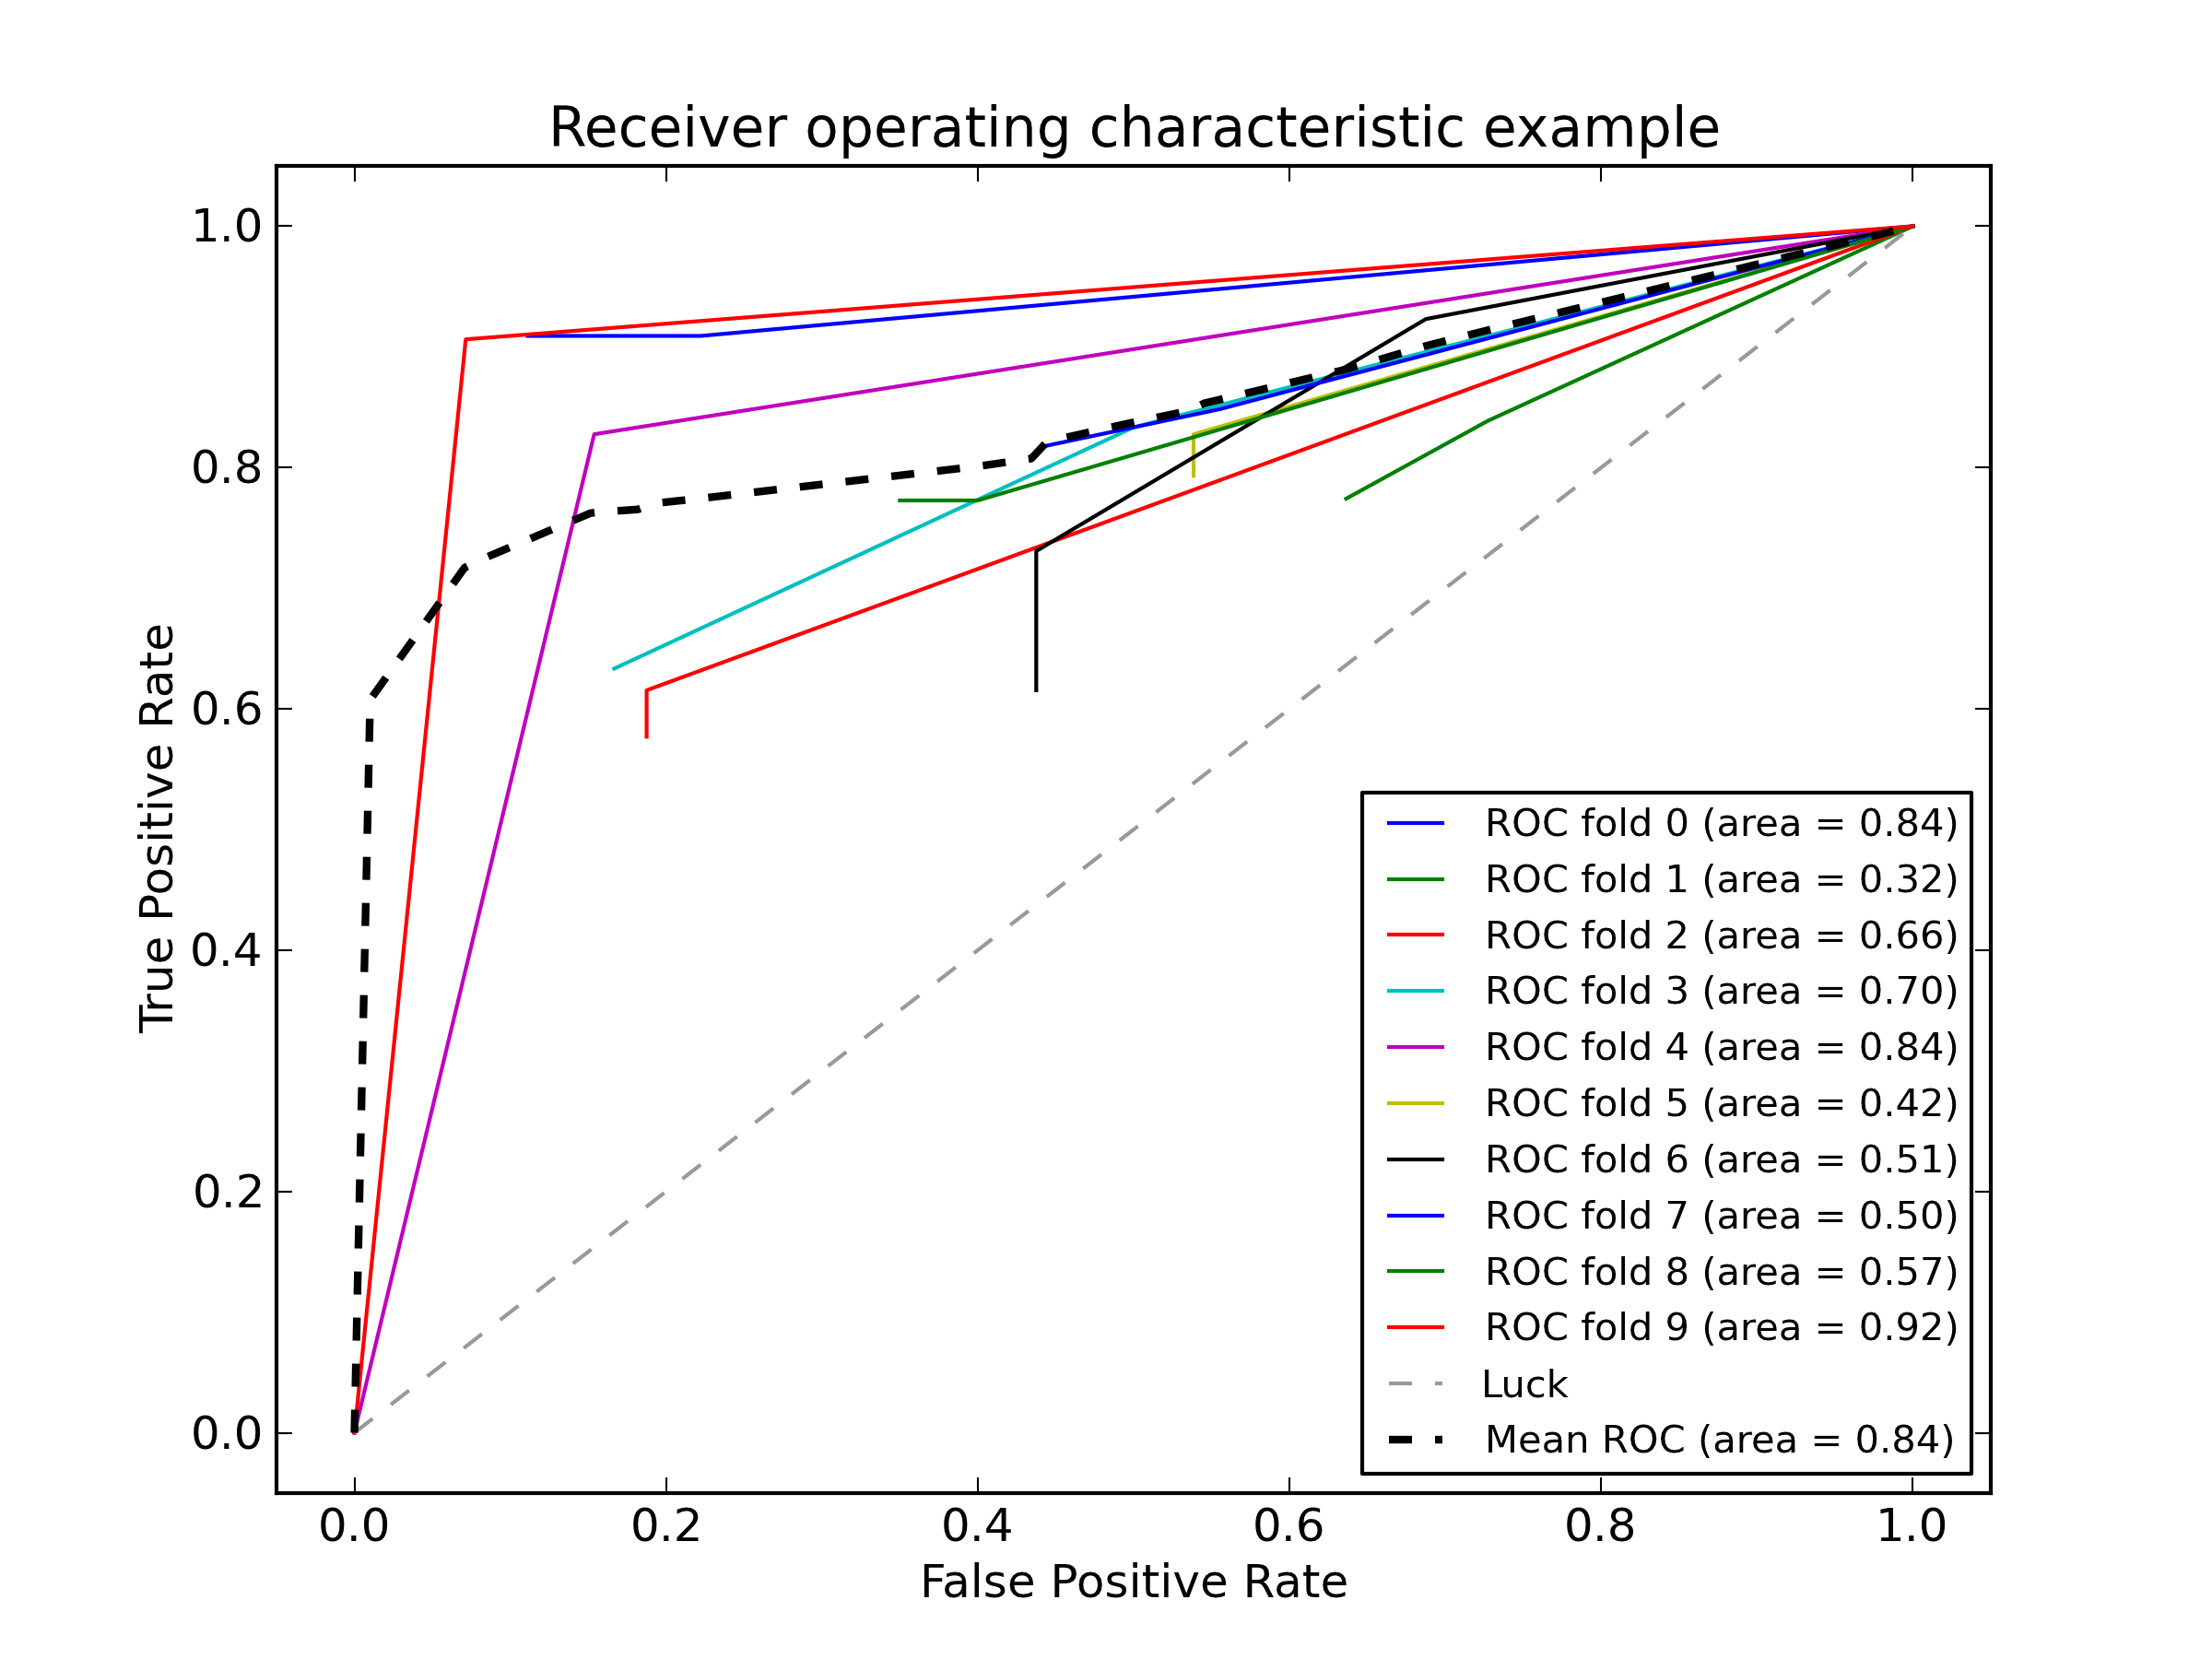
\includegraphics[width=0.36\textwidth]{pics/0_590_dtree.png}}
\quad
\subfloat[Multinomial Bayes]{
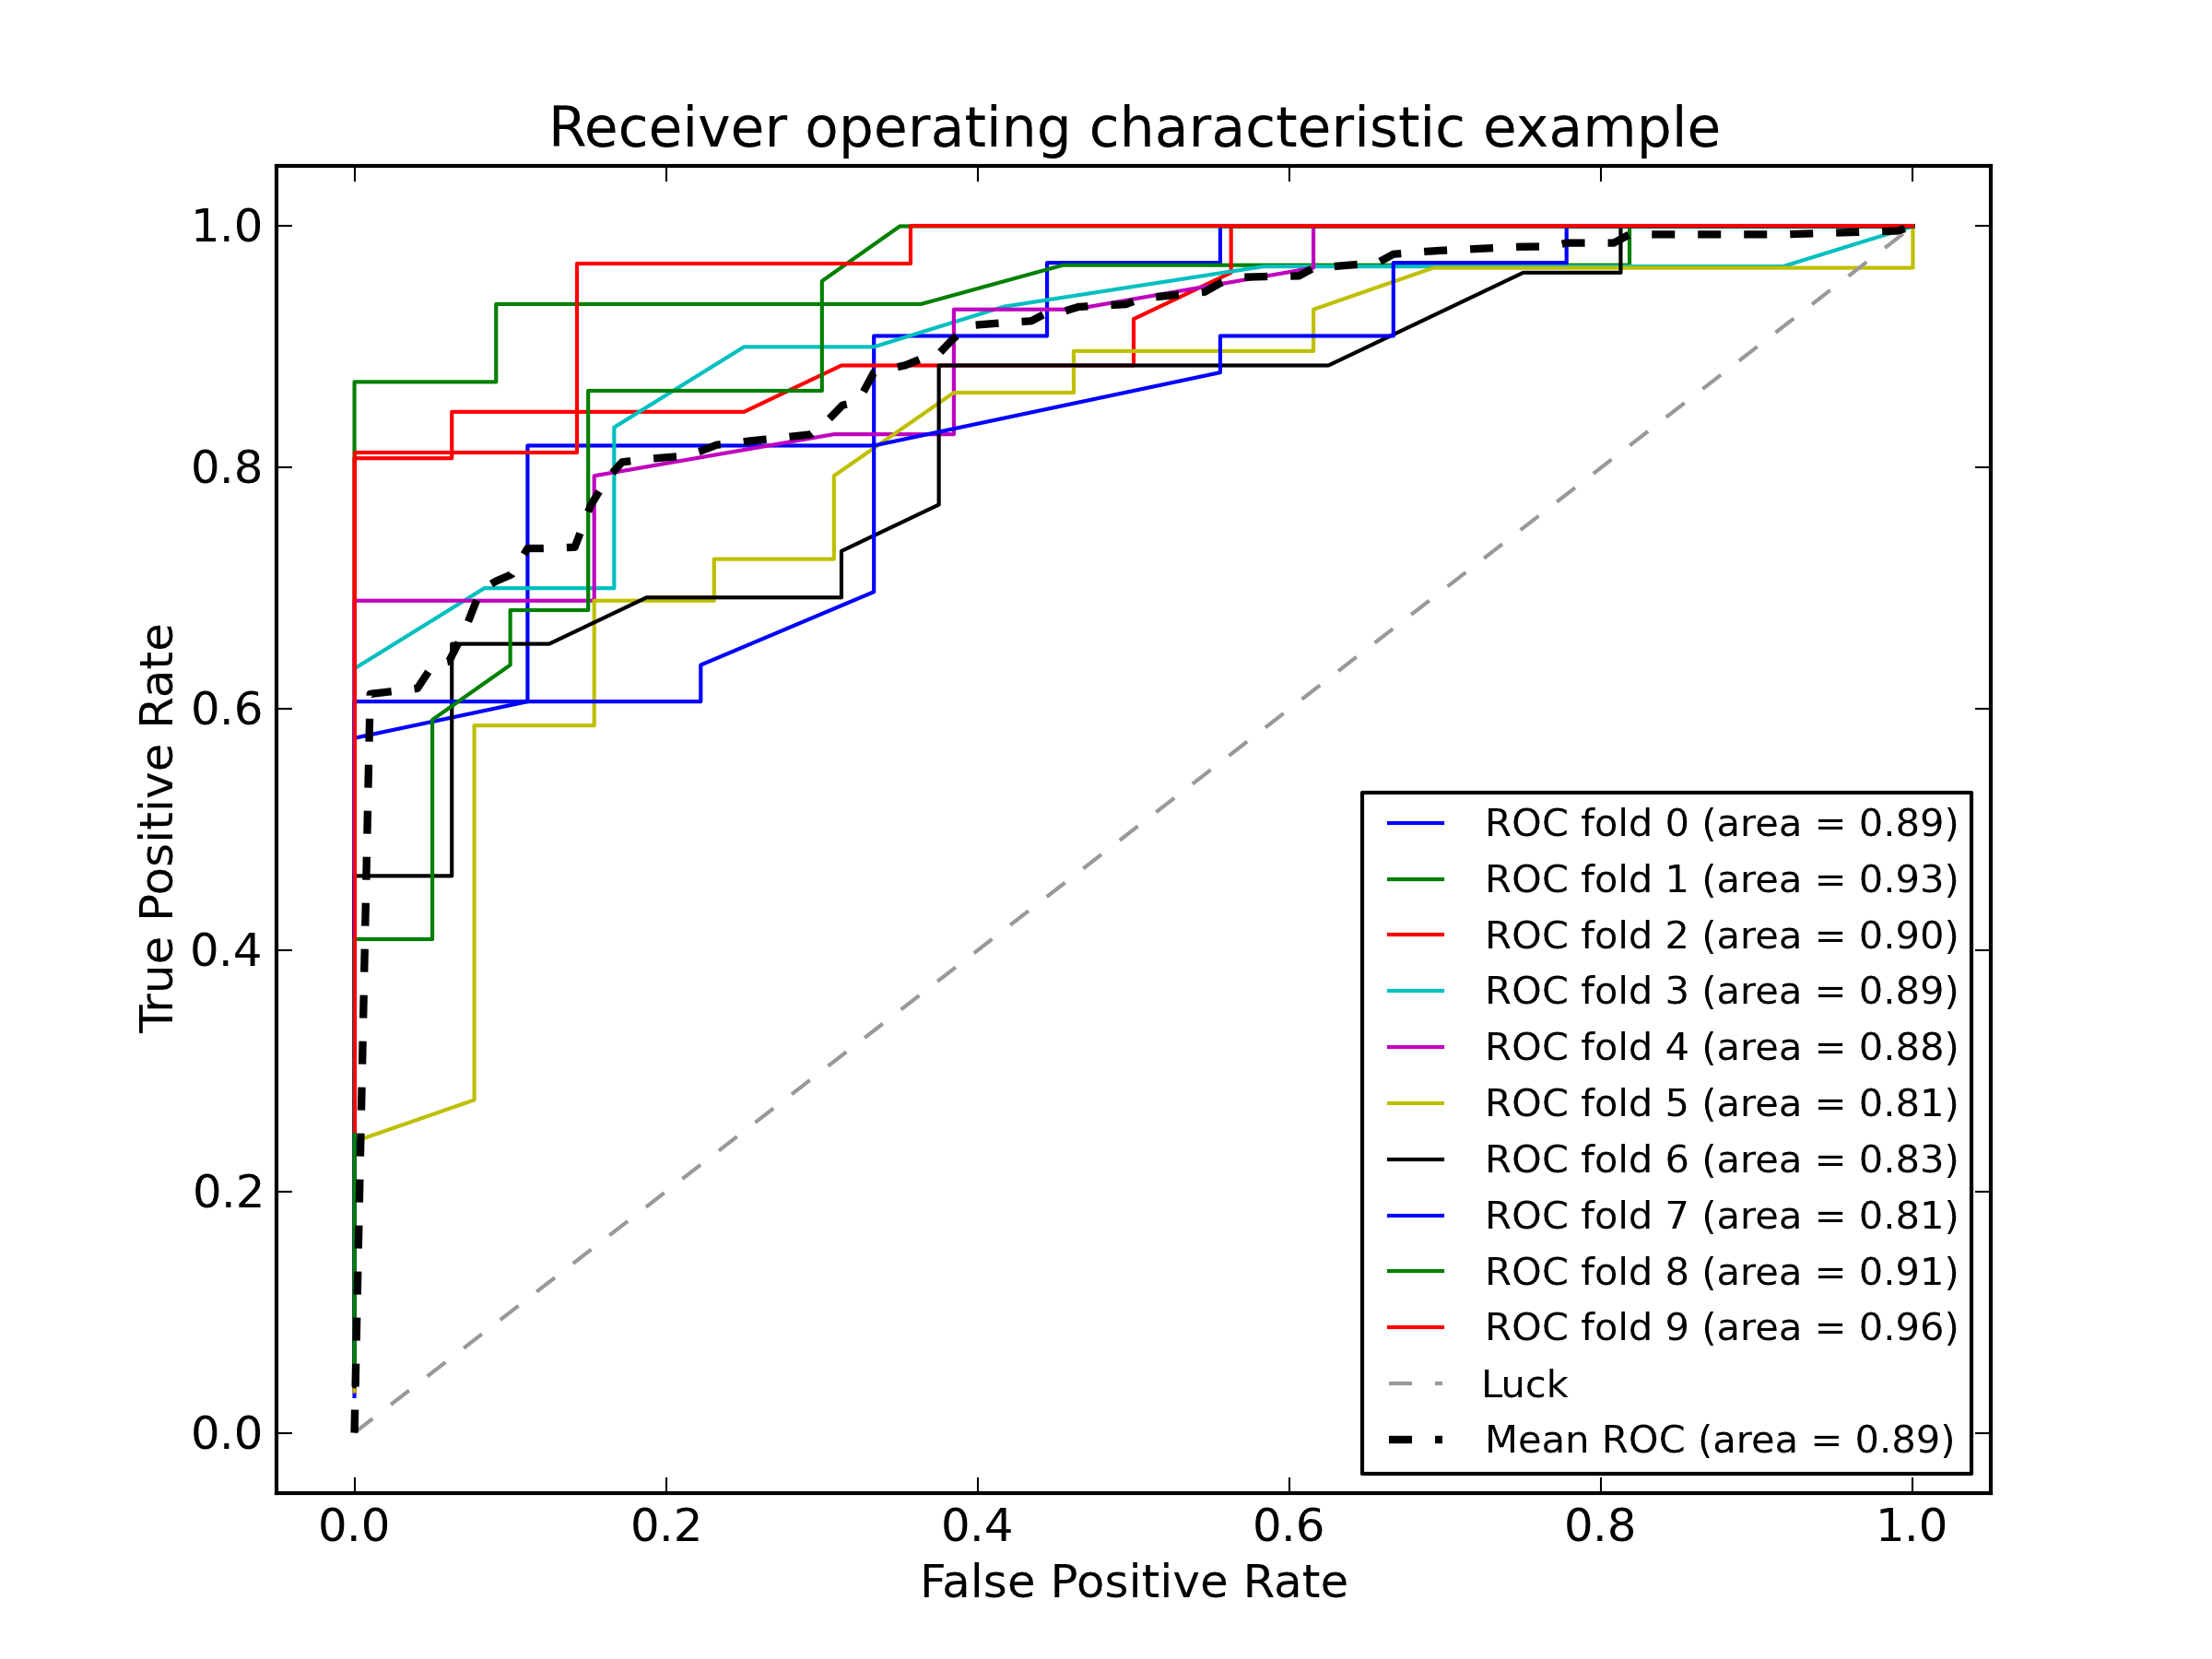
\includegraphics[width=0.36\textwidth]{pics/0_590_multi.png}}
\quad
\subfloat[Support Vector Machines]{
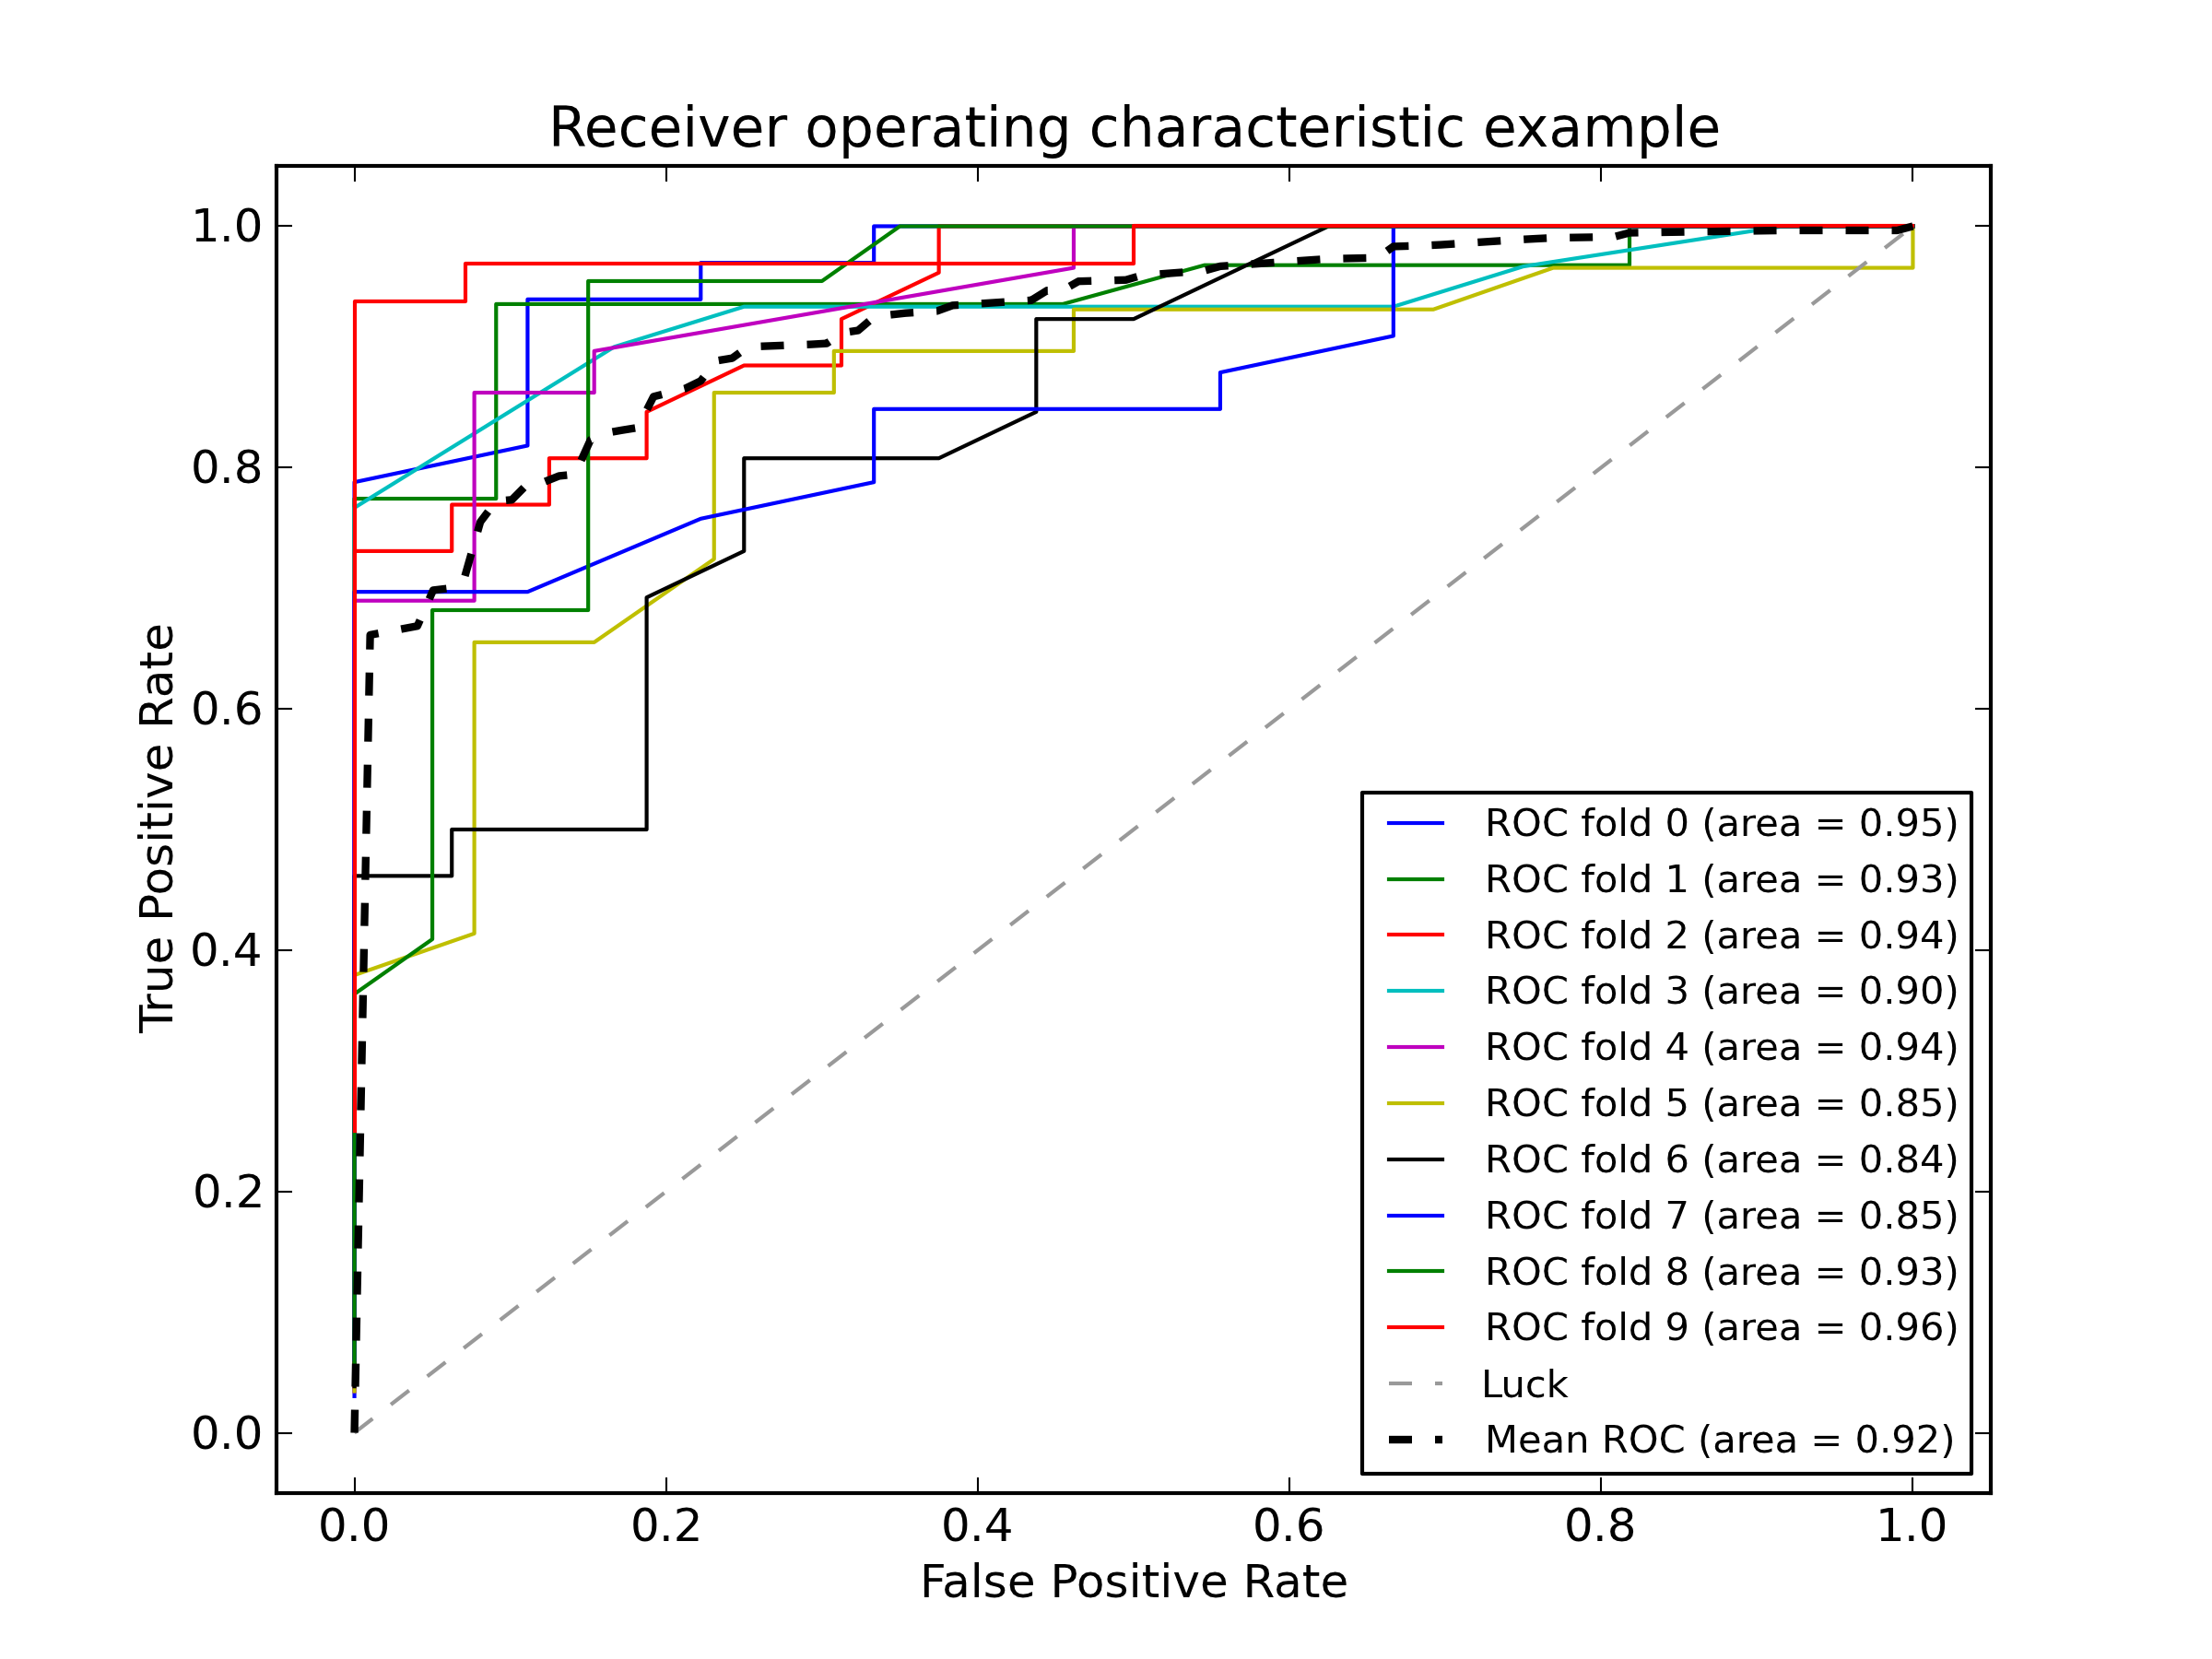
\includegraphics[width=0.36\textwidth]{pics/0_590_svm.png}}
\quad
\subfloat[Random Forests]{
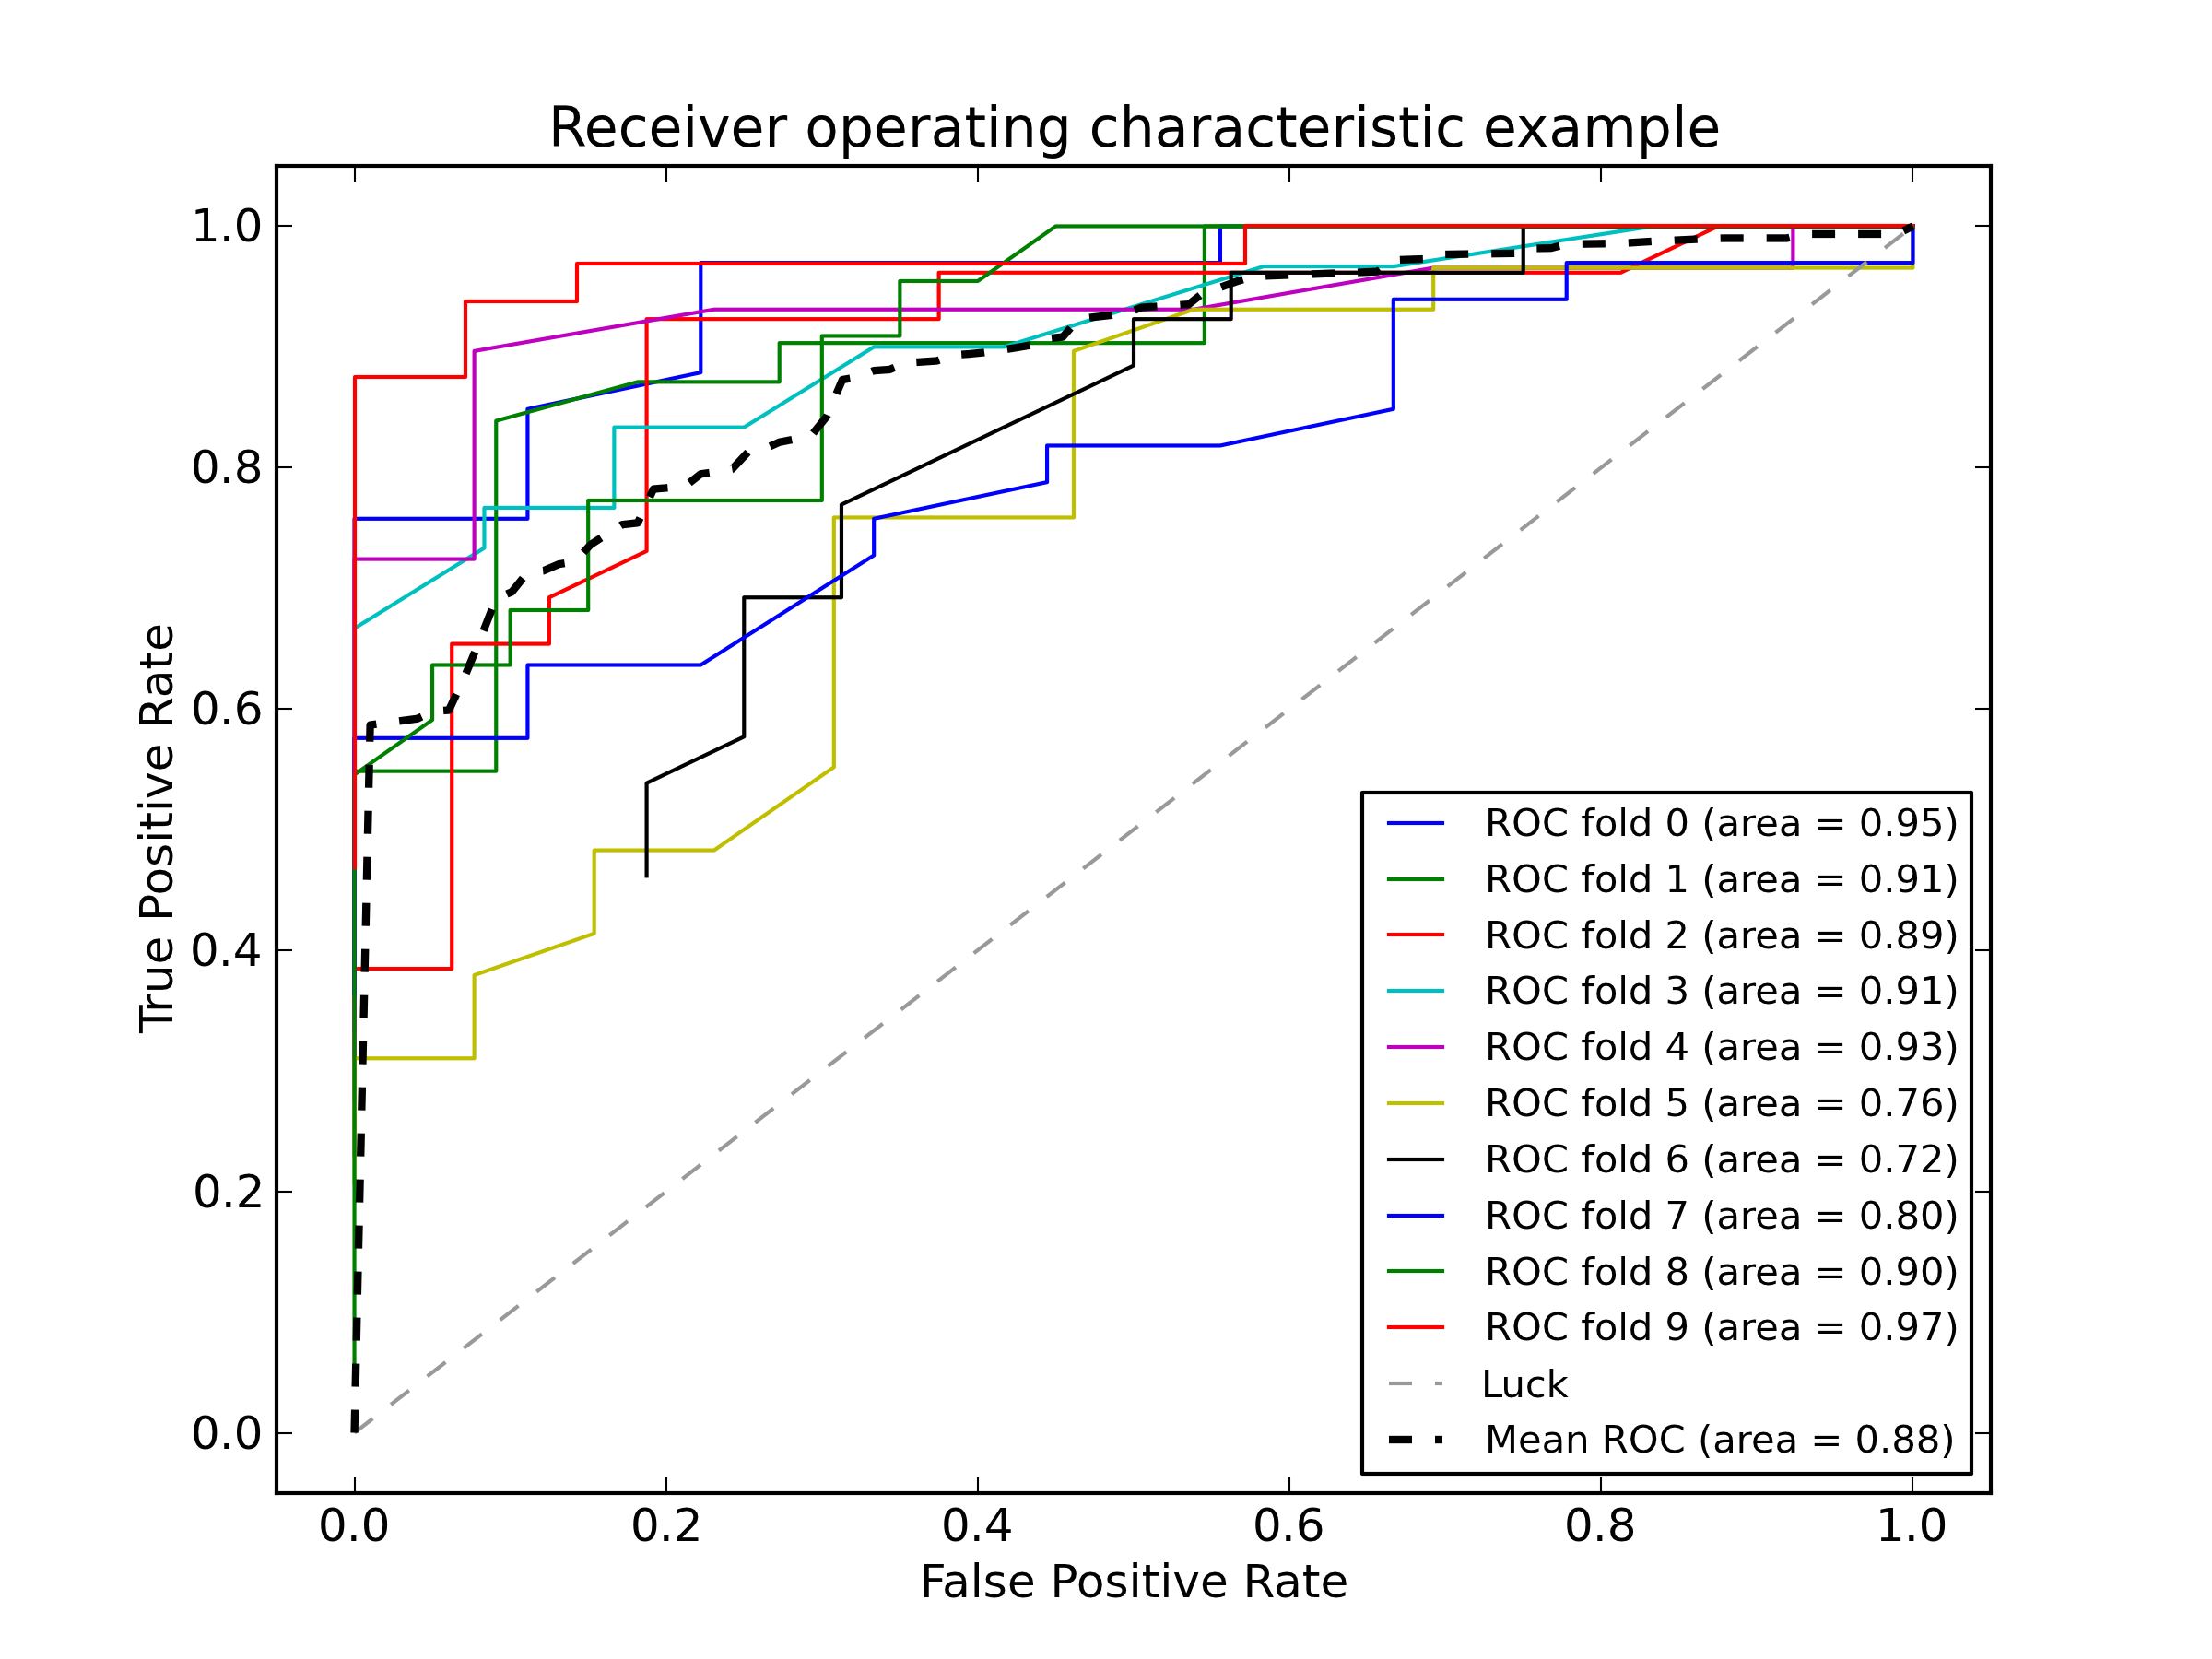
\includegraphics[width=0.36\textwidth]{pics/0_590_forest.png}}
\quad
\subfloat[Stacking - Logistic Regression]{
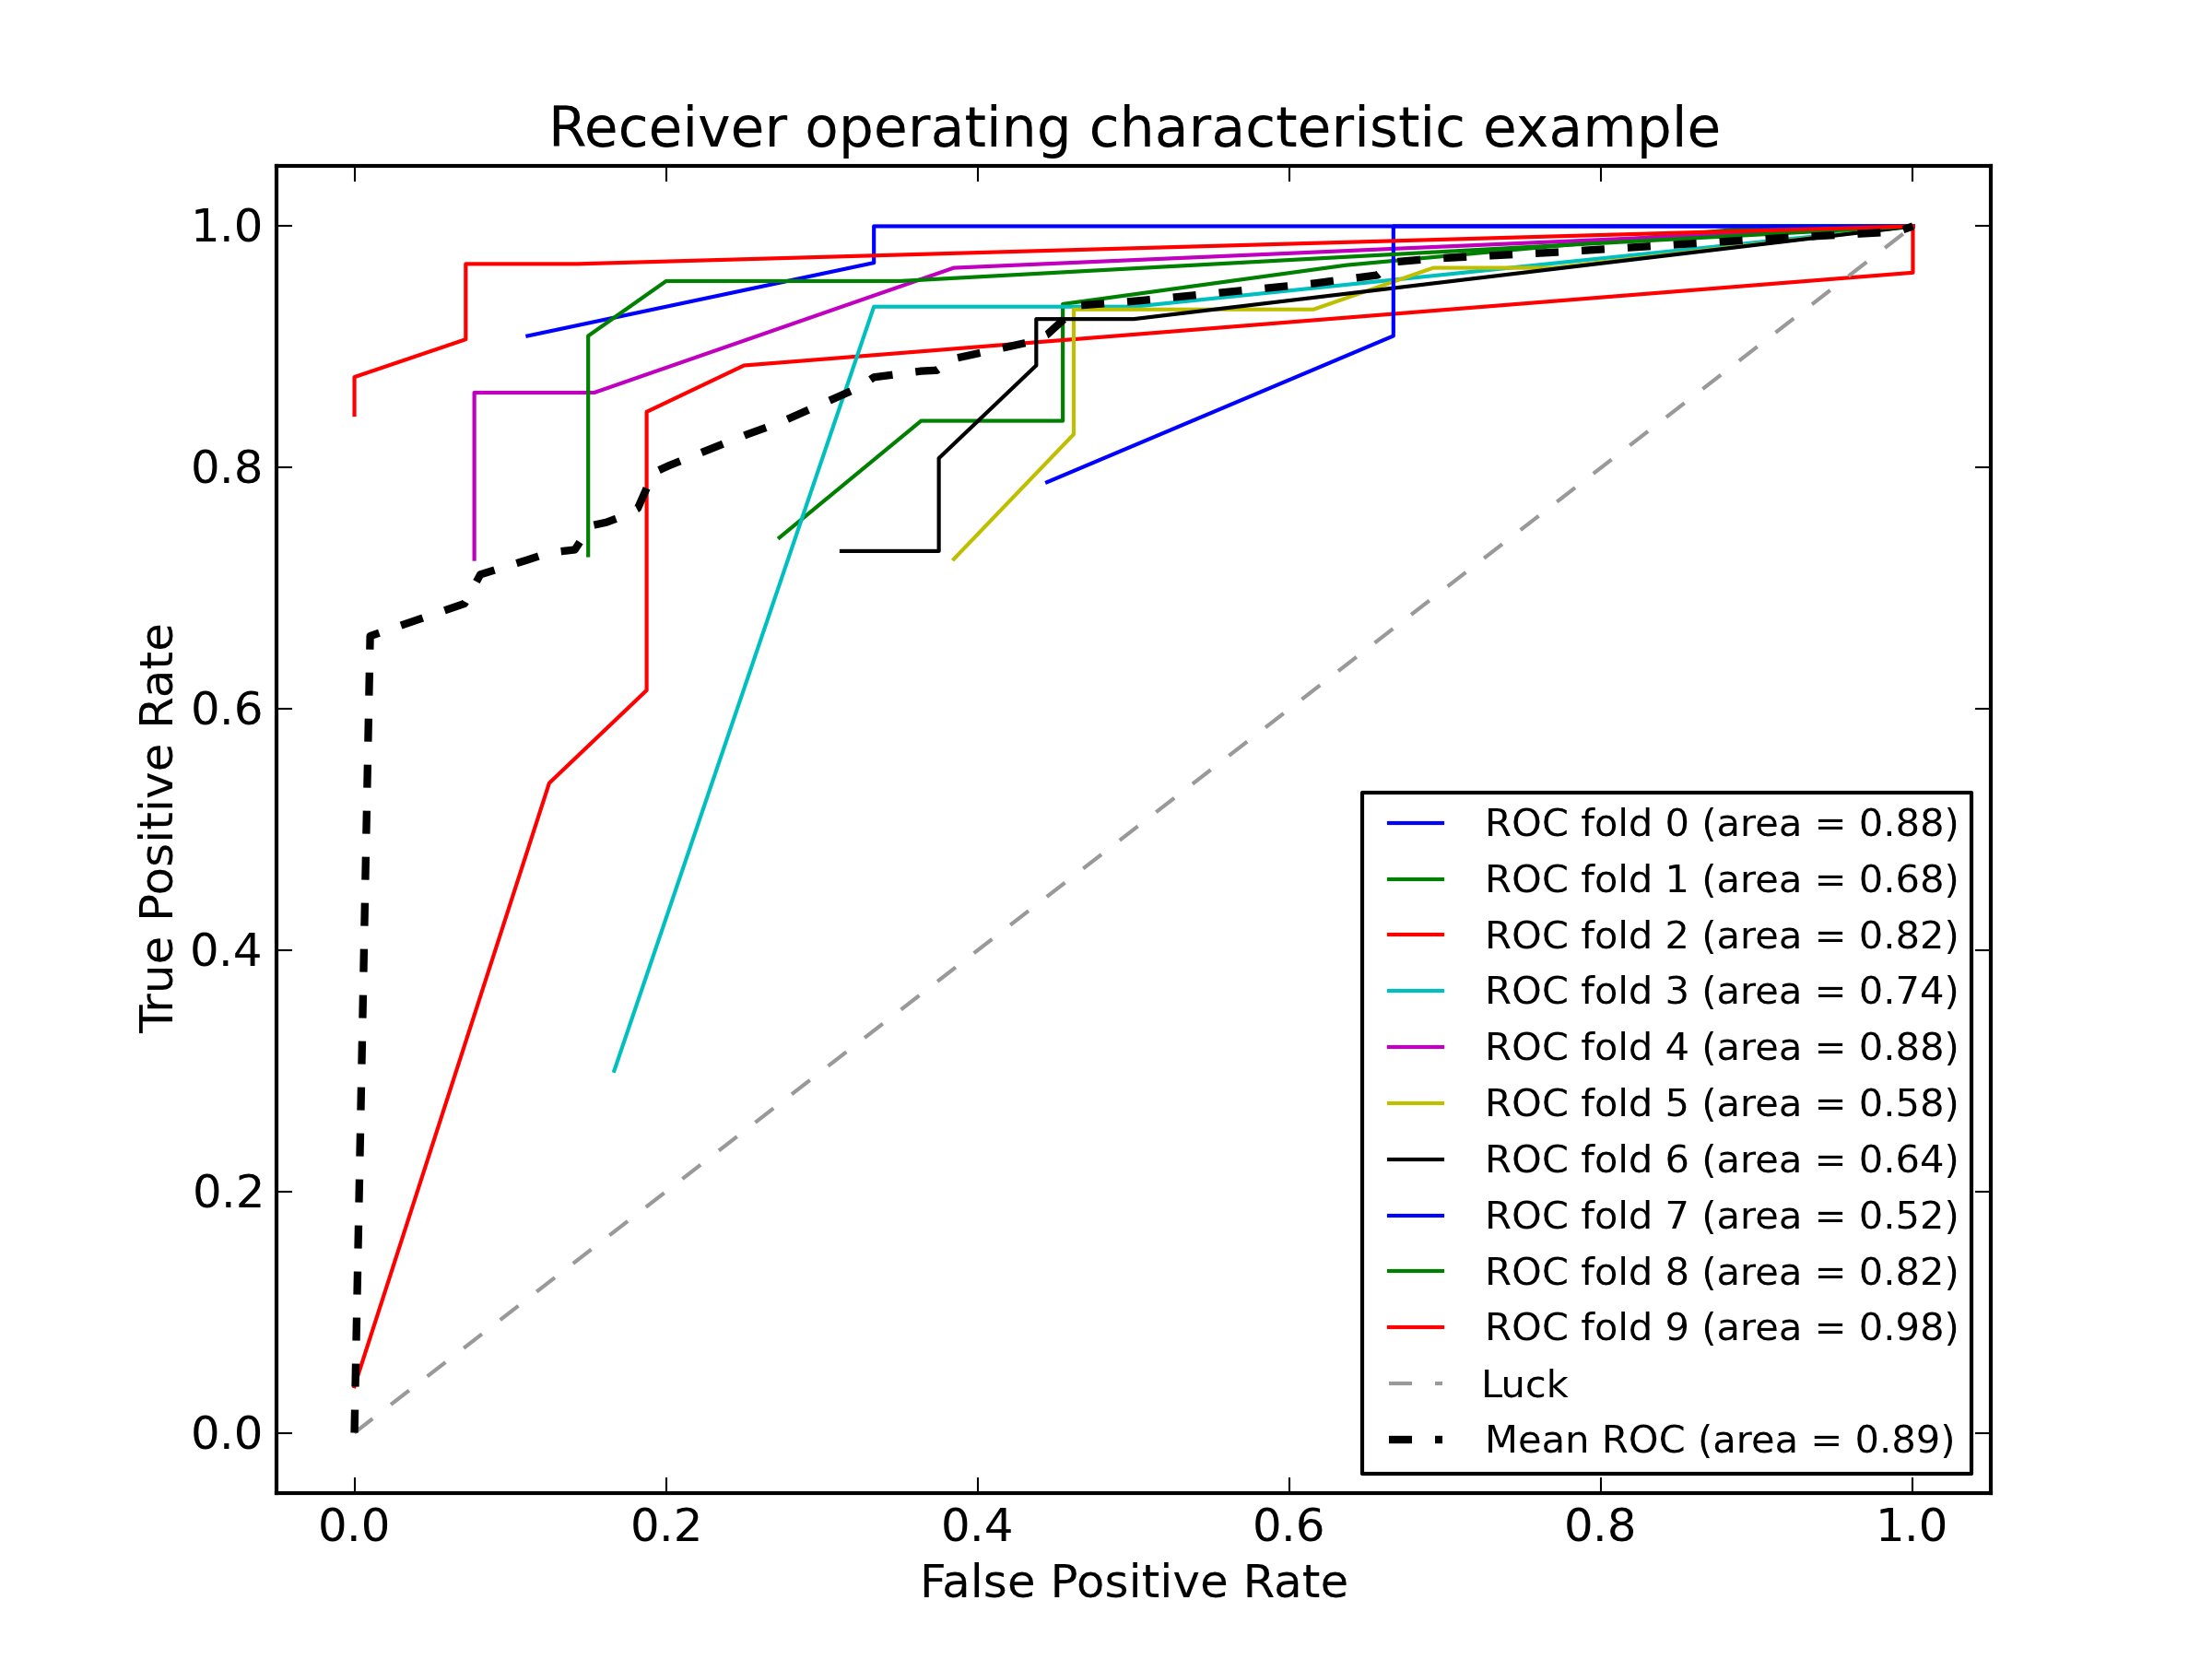
\includegraphics[width=0.36\textwidth]{pics/0_590_wmm.png}}
\quad
\subfloat[Stacking - Multi-Response Linear Models]{
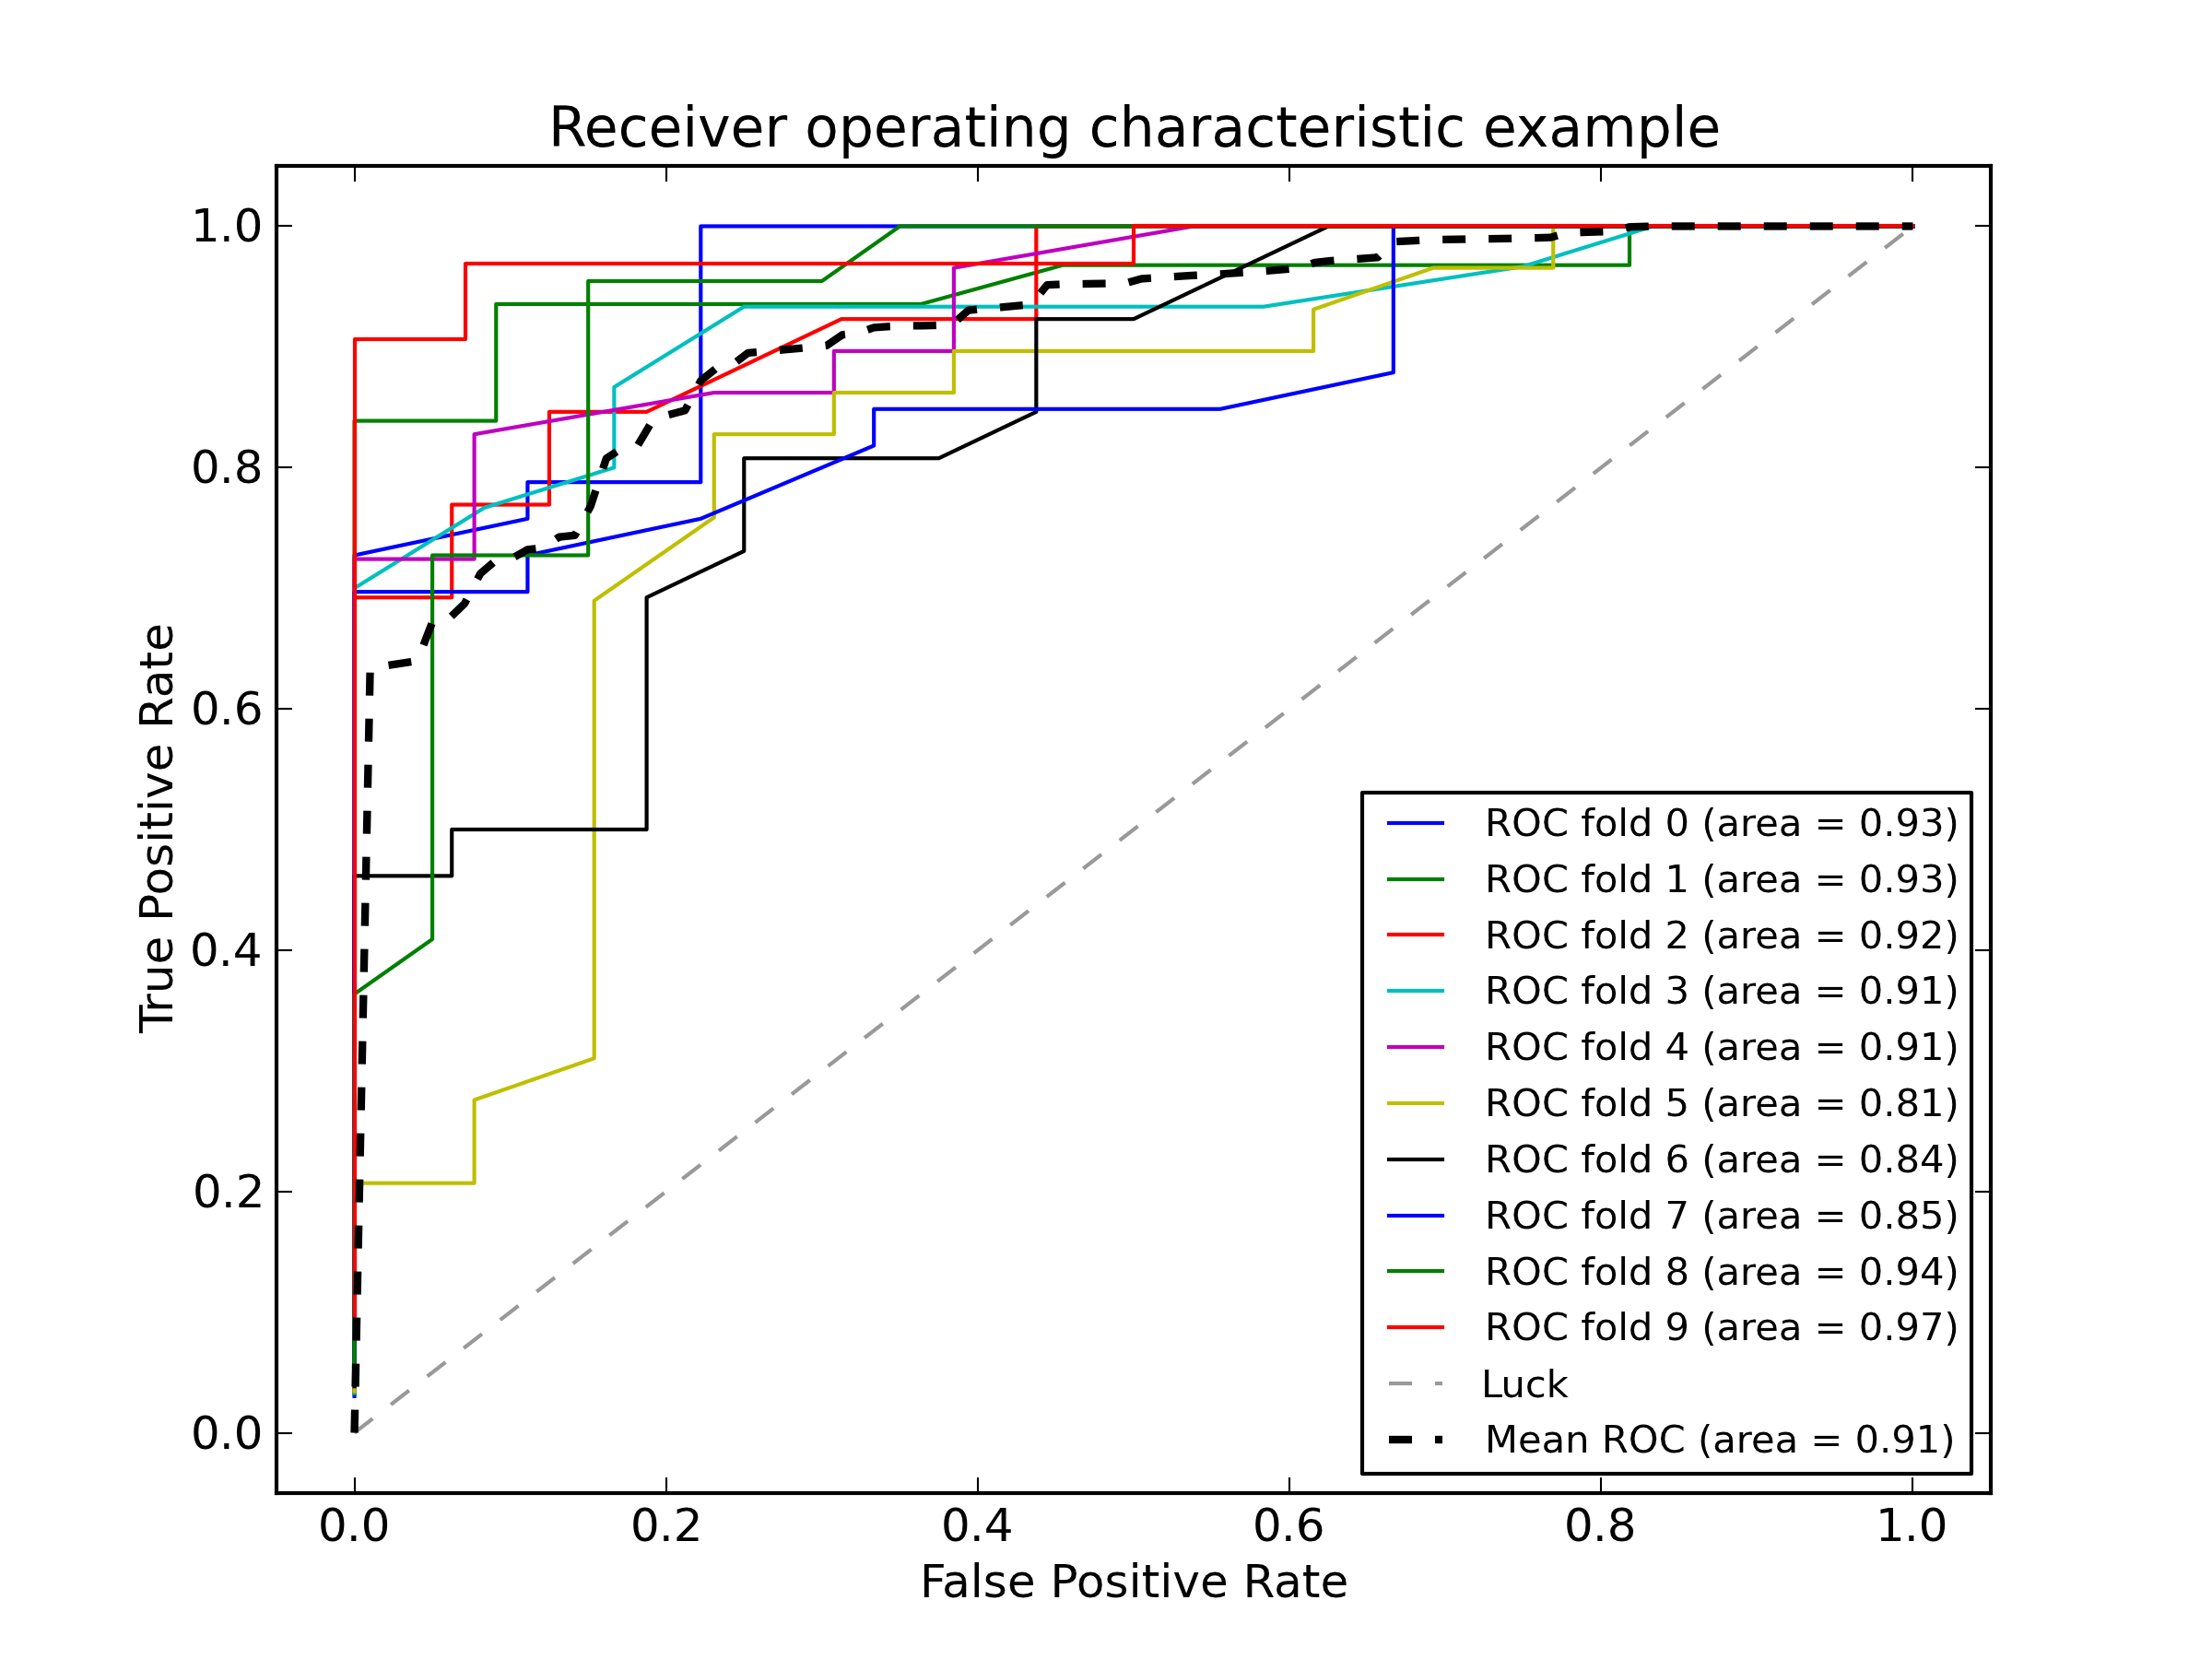
\includegraphics[width=0.36\textwidth]{pics/0_590_smm.png}}
\caption{Results for Features 1-4}
\label{fig:fig1}
\end{figure}

\begin{figure}[t]
\centering
\subfloat[Logistic Regression]{
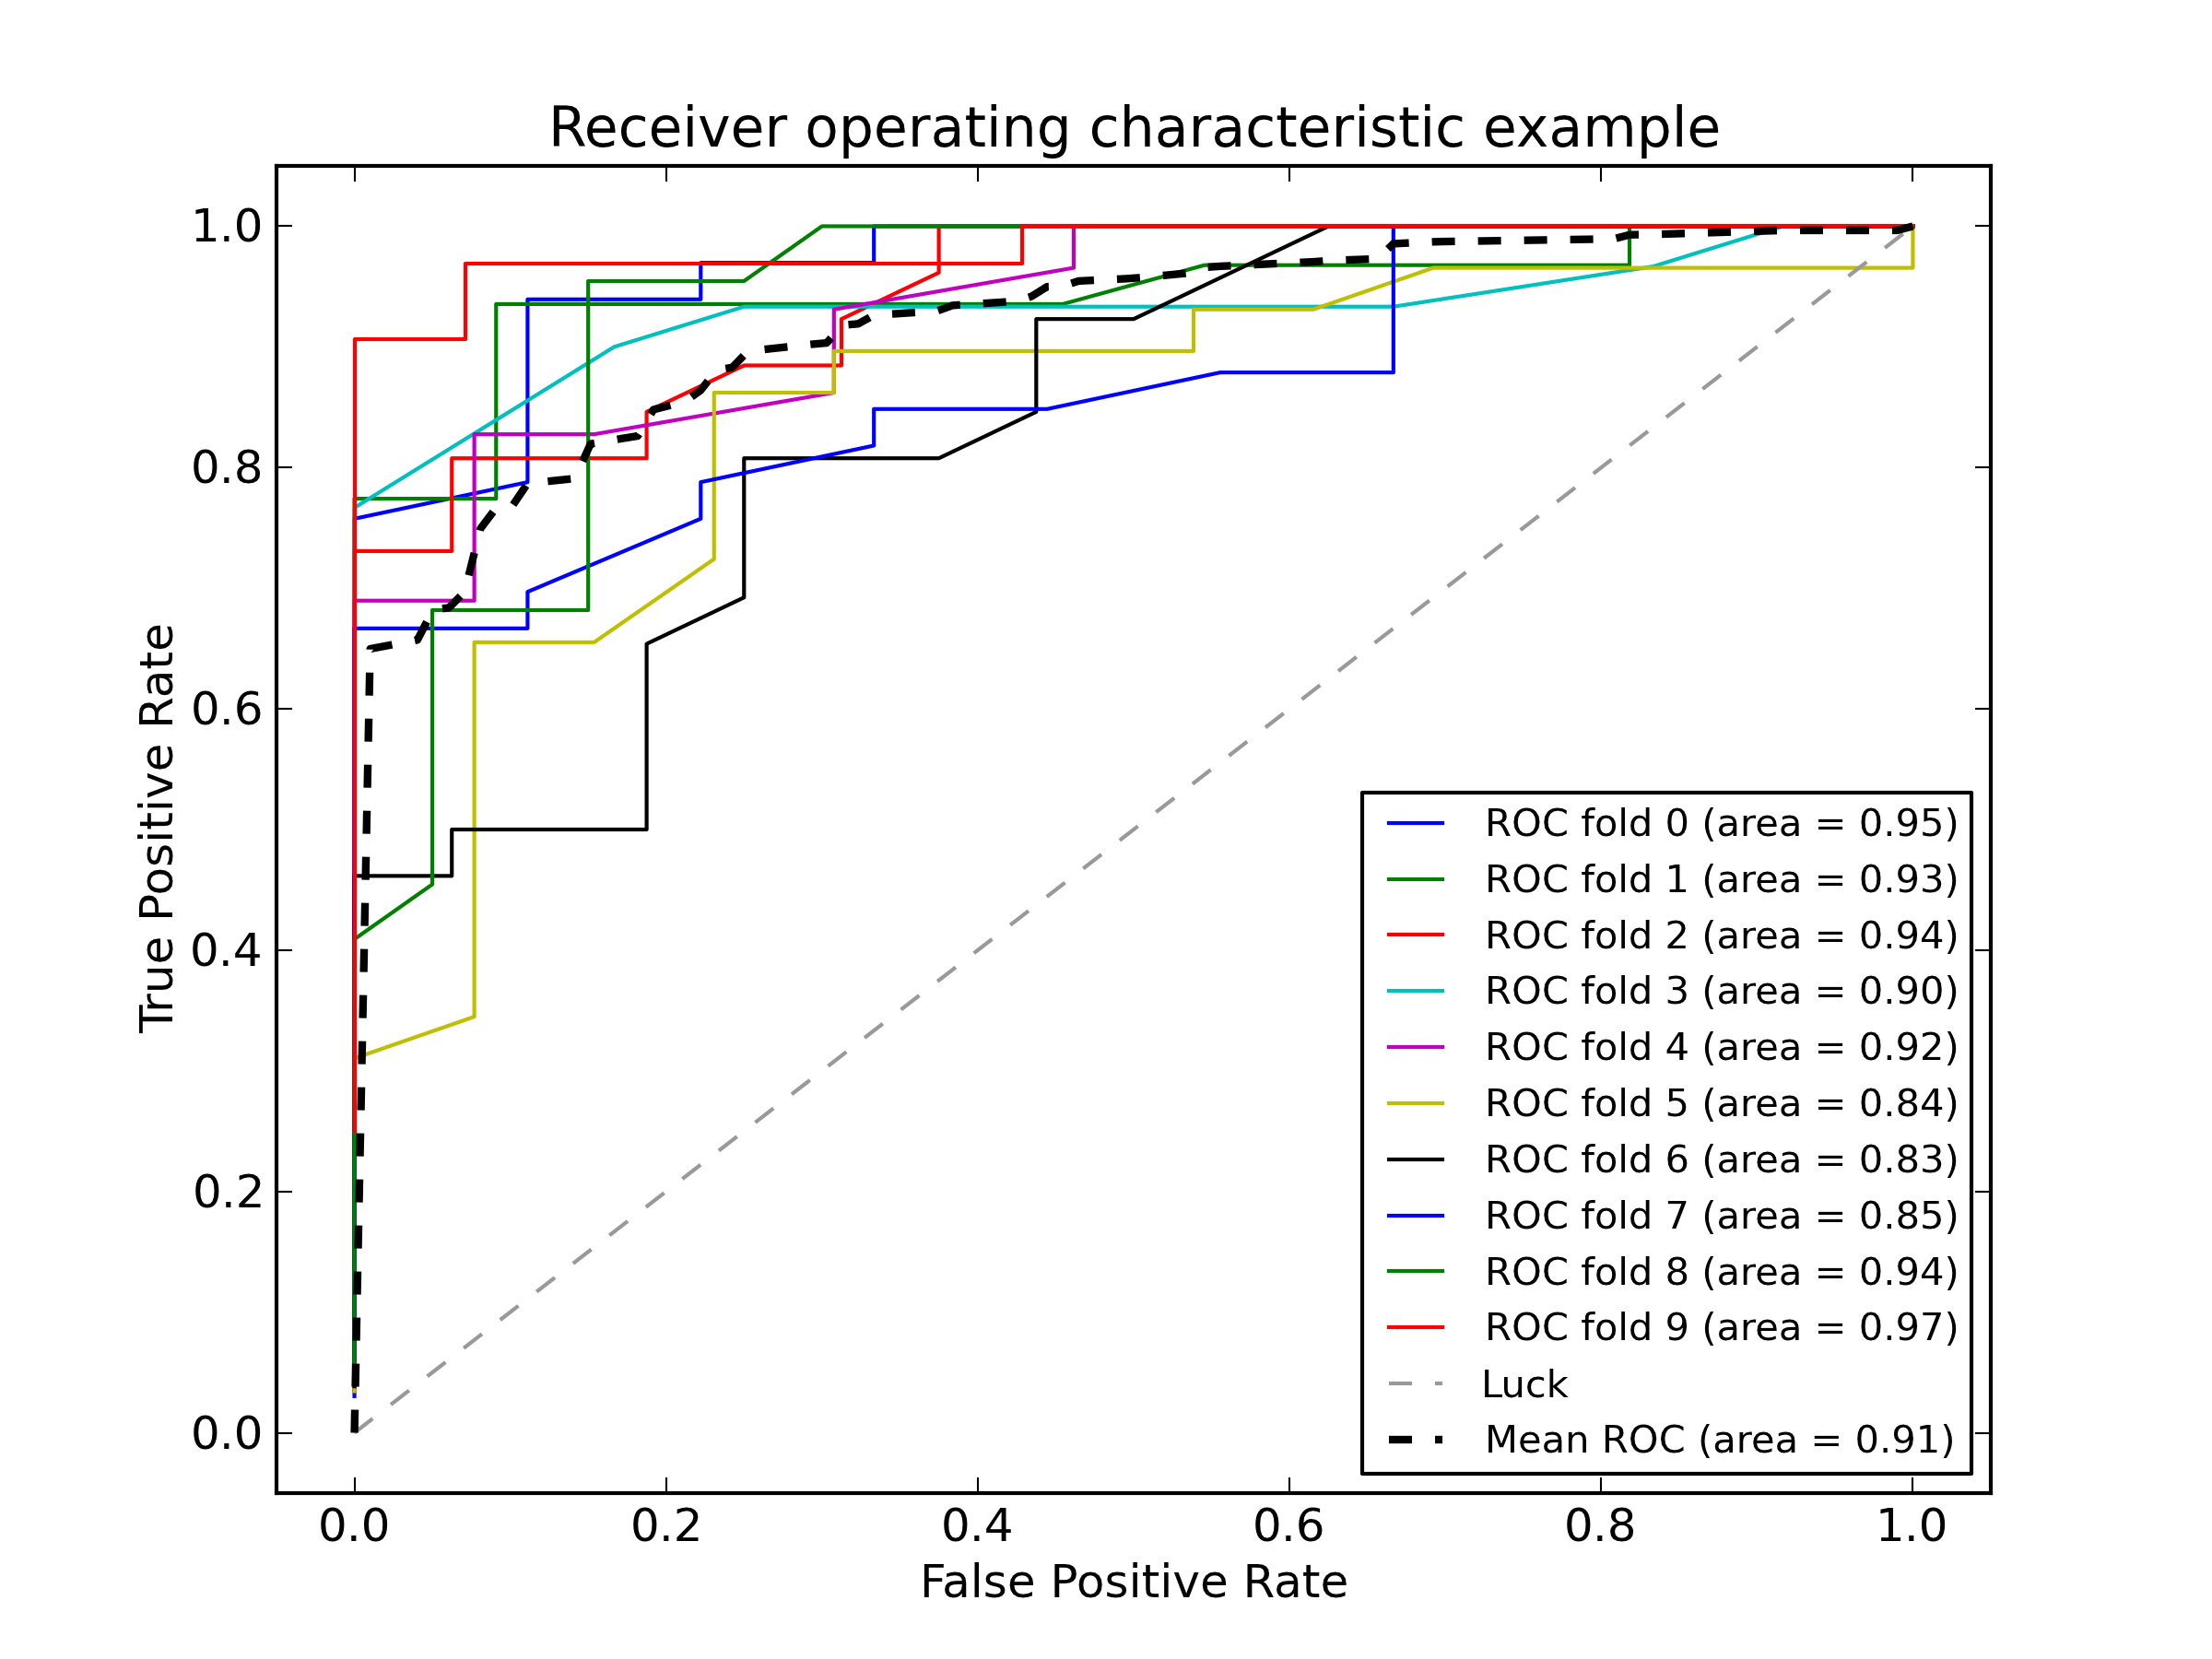
\includegraphics[width=0.36\textwidth]{pics/1_590_logit.png}}
\quad
\subfloat[Decision Trees]{
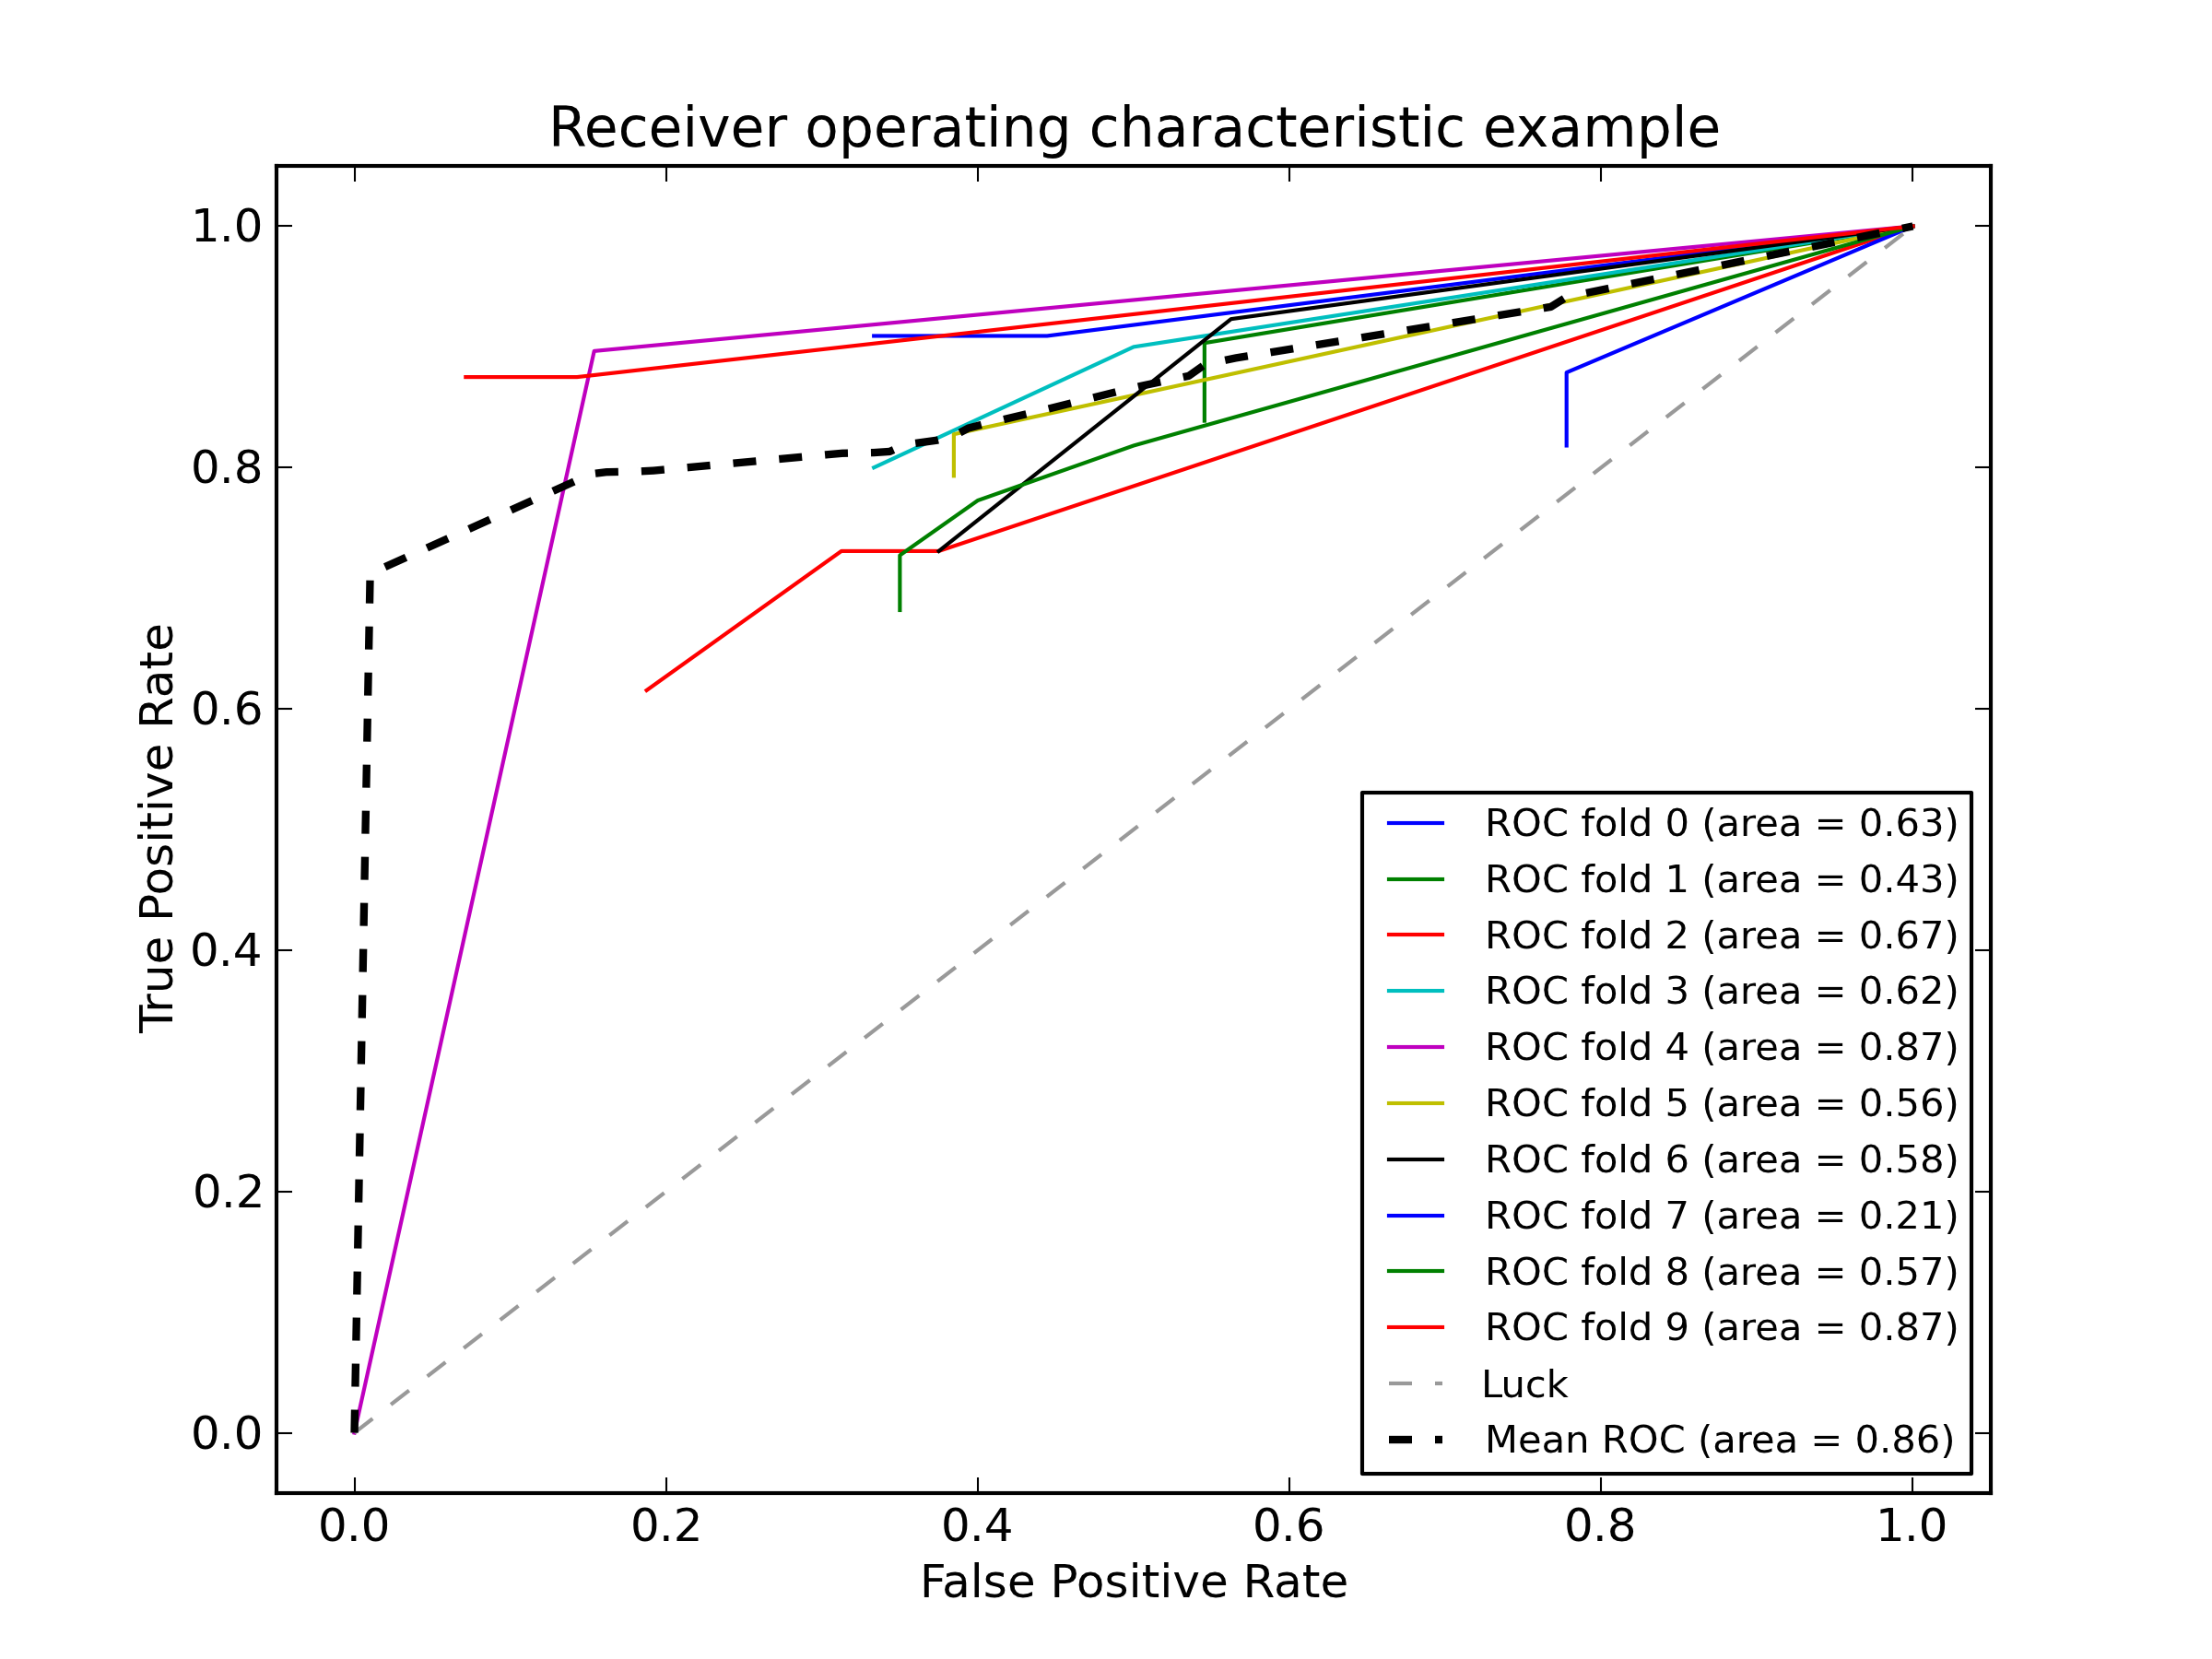
\includegraphics[width=0.36\textwidth]{pics/1_590_dtree.png}}
\quad
\subfloat[Multinomial Bayes]{
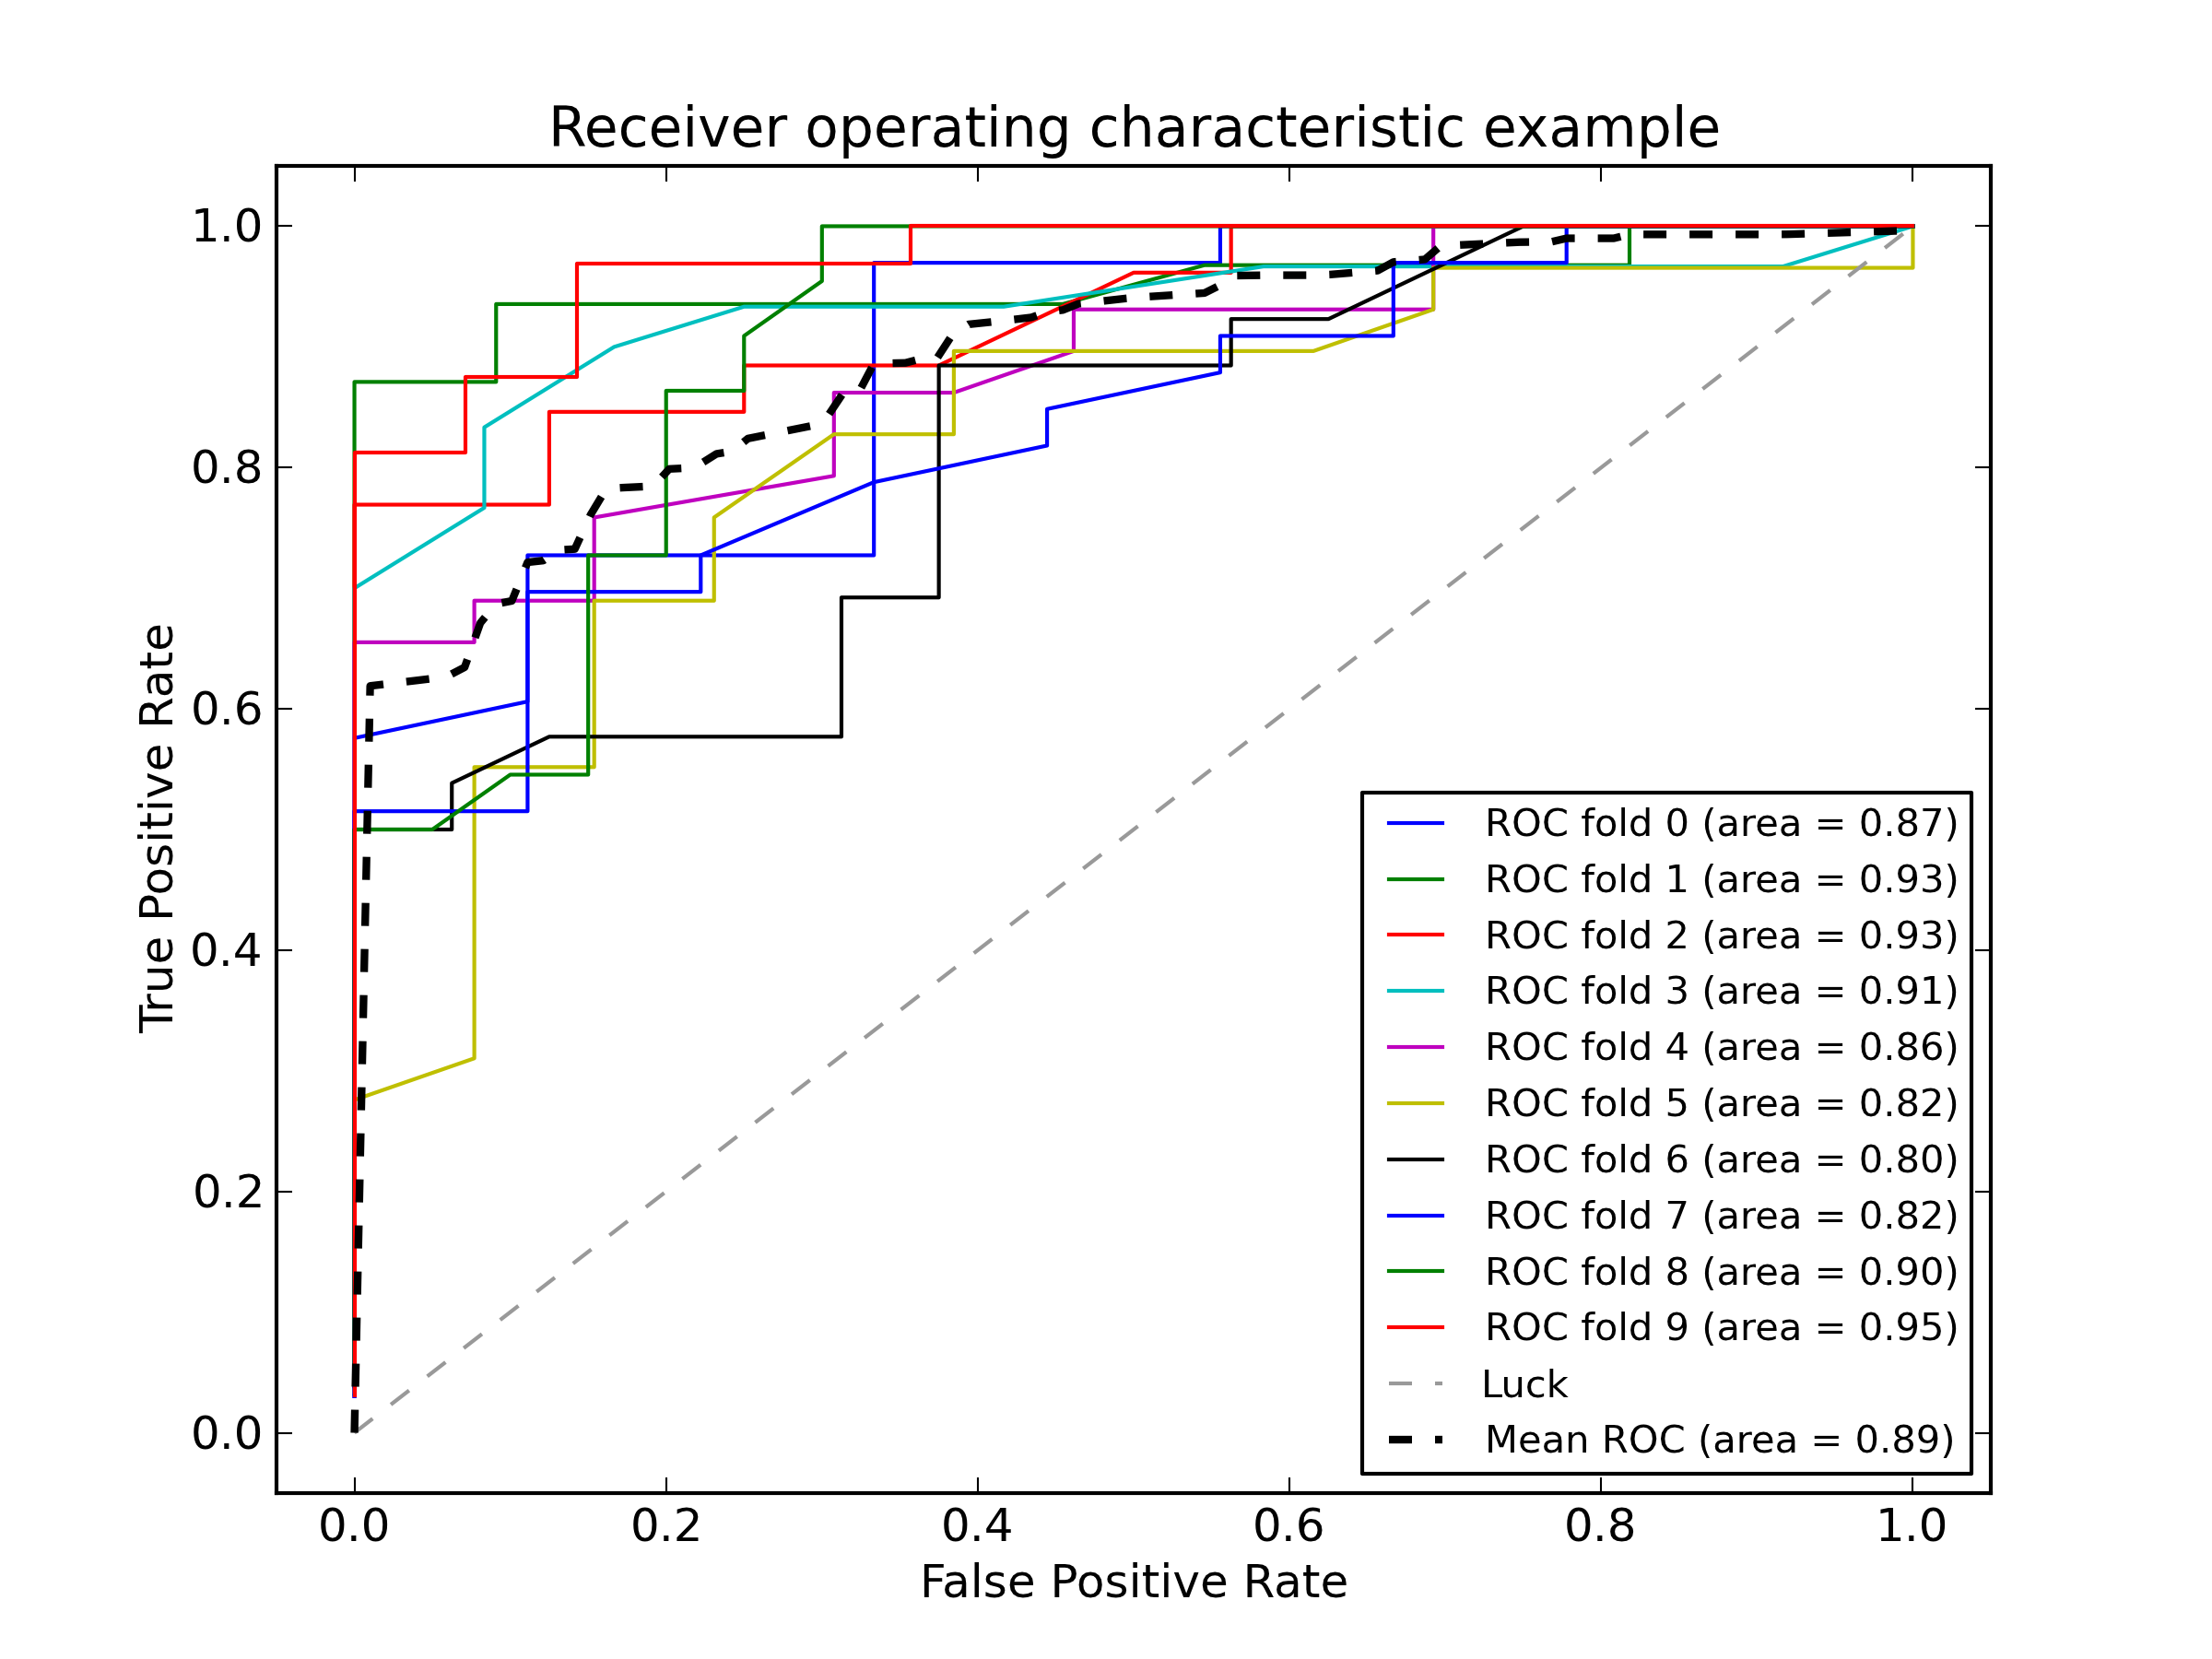
\includegraphics[width=0.36\textwidth]{pics/1_590_multi.png}}
\quad
\subfloat[Support Vector Machines]{
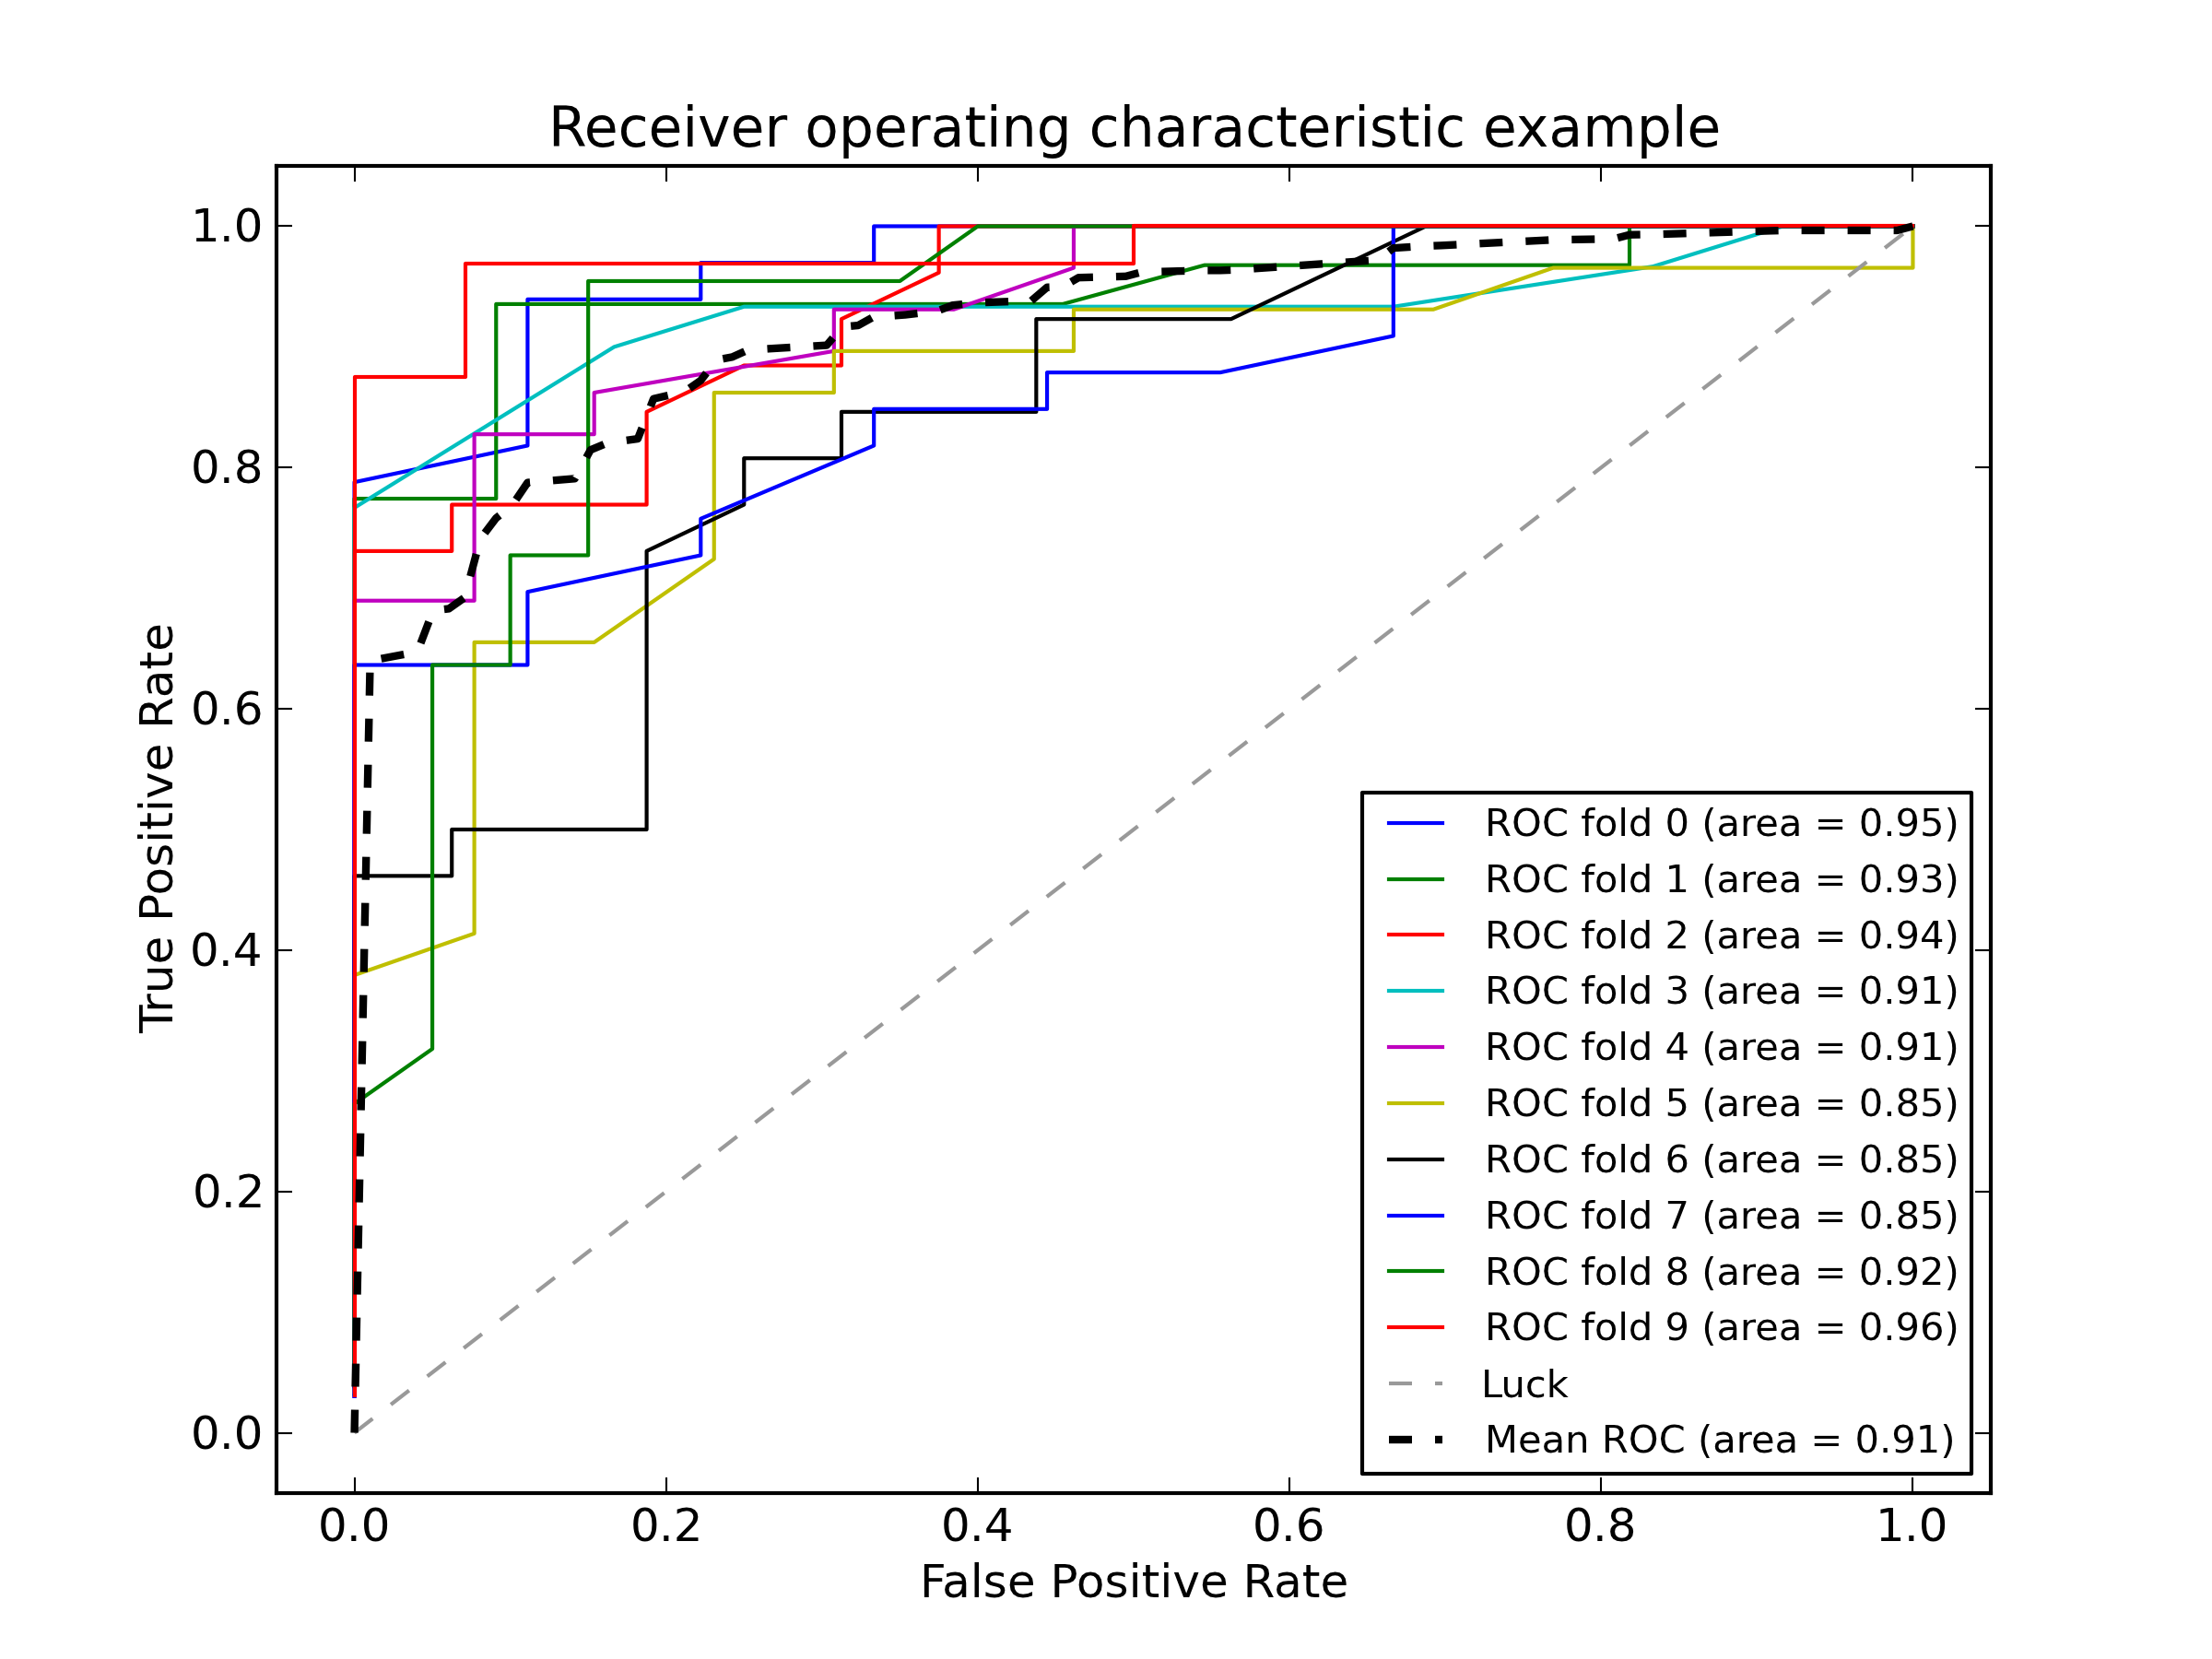
\includegraphics[width=0.36\textwidth]{pics/1_590_svm.png}}
\quad
\subfloat[Random Forests]{
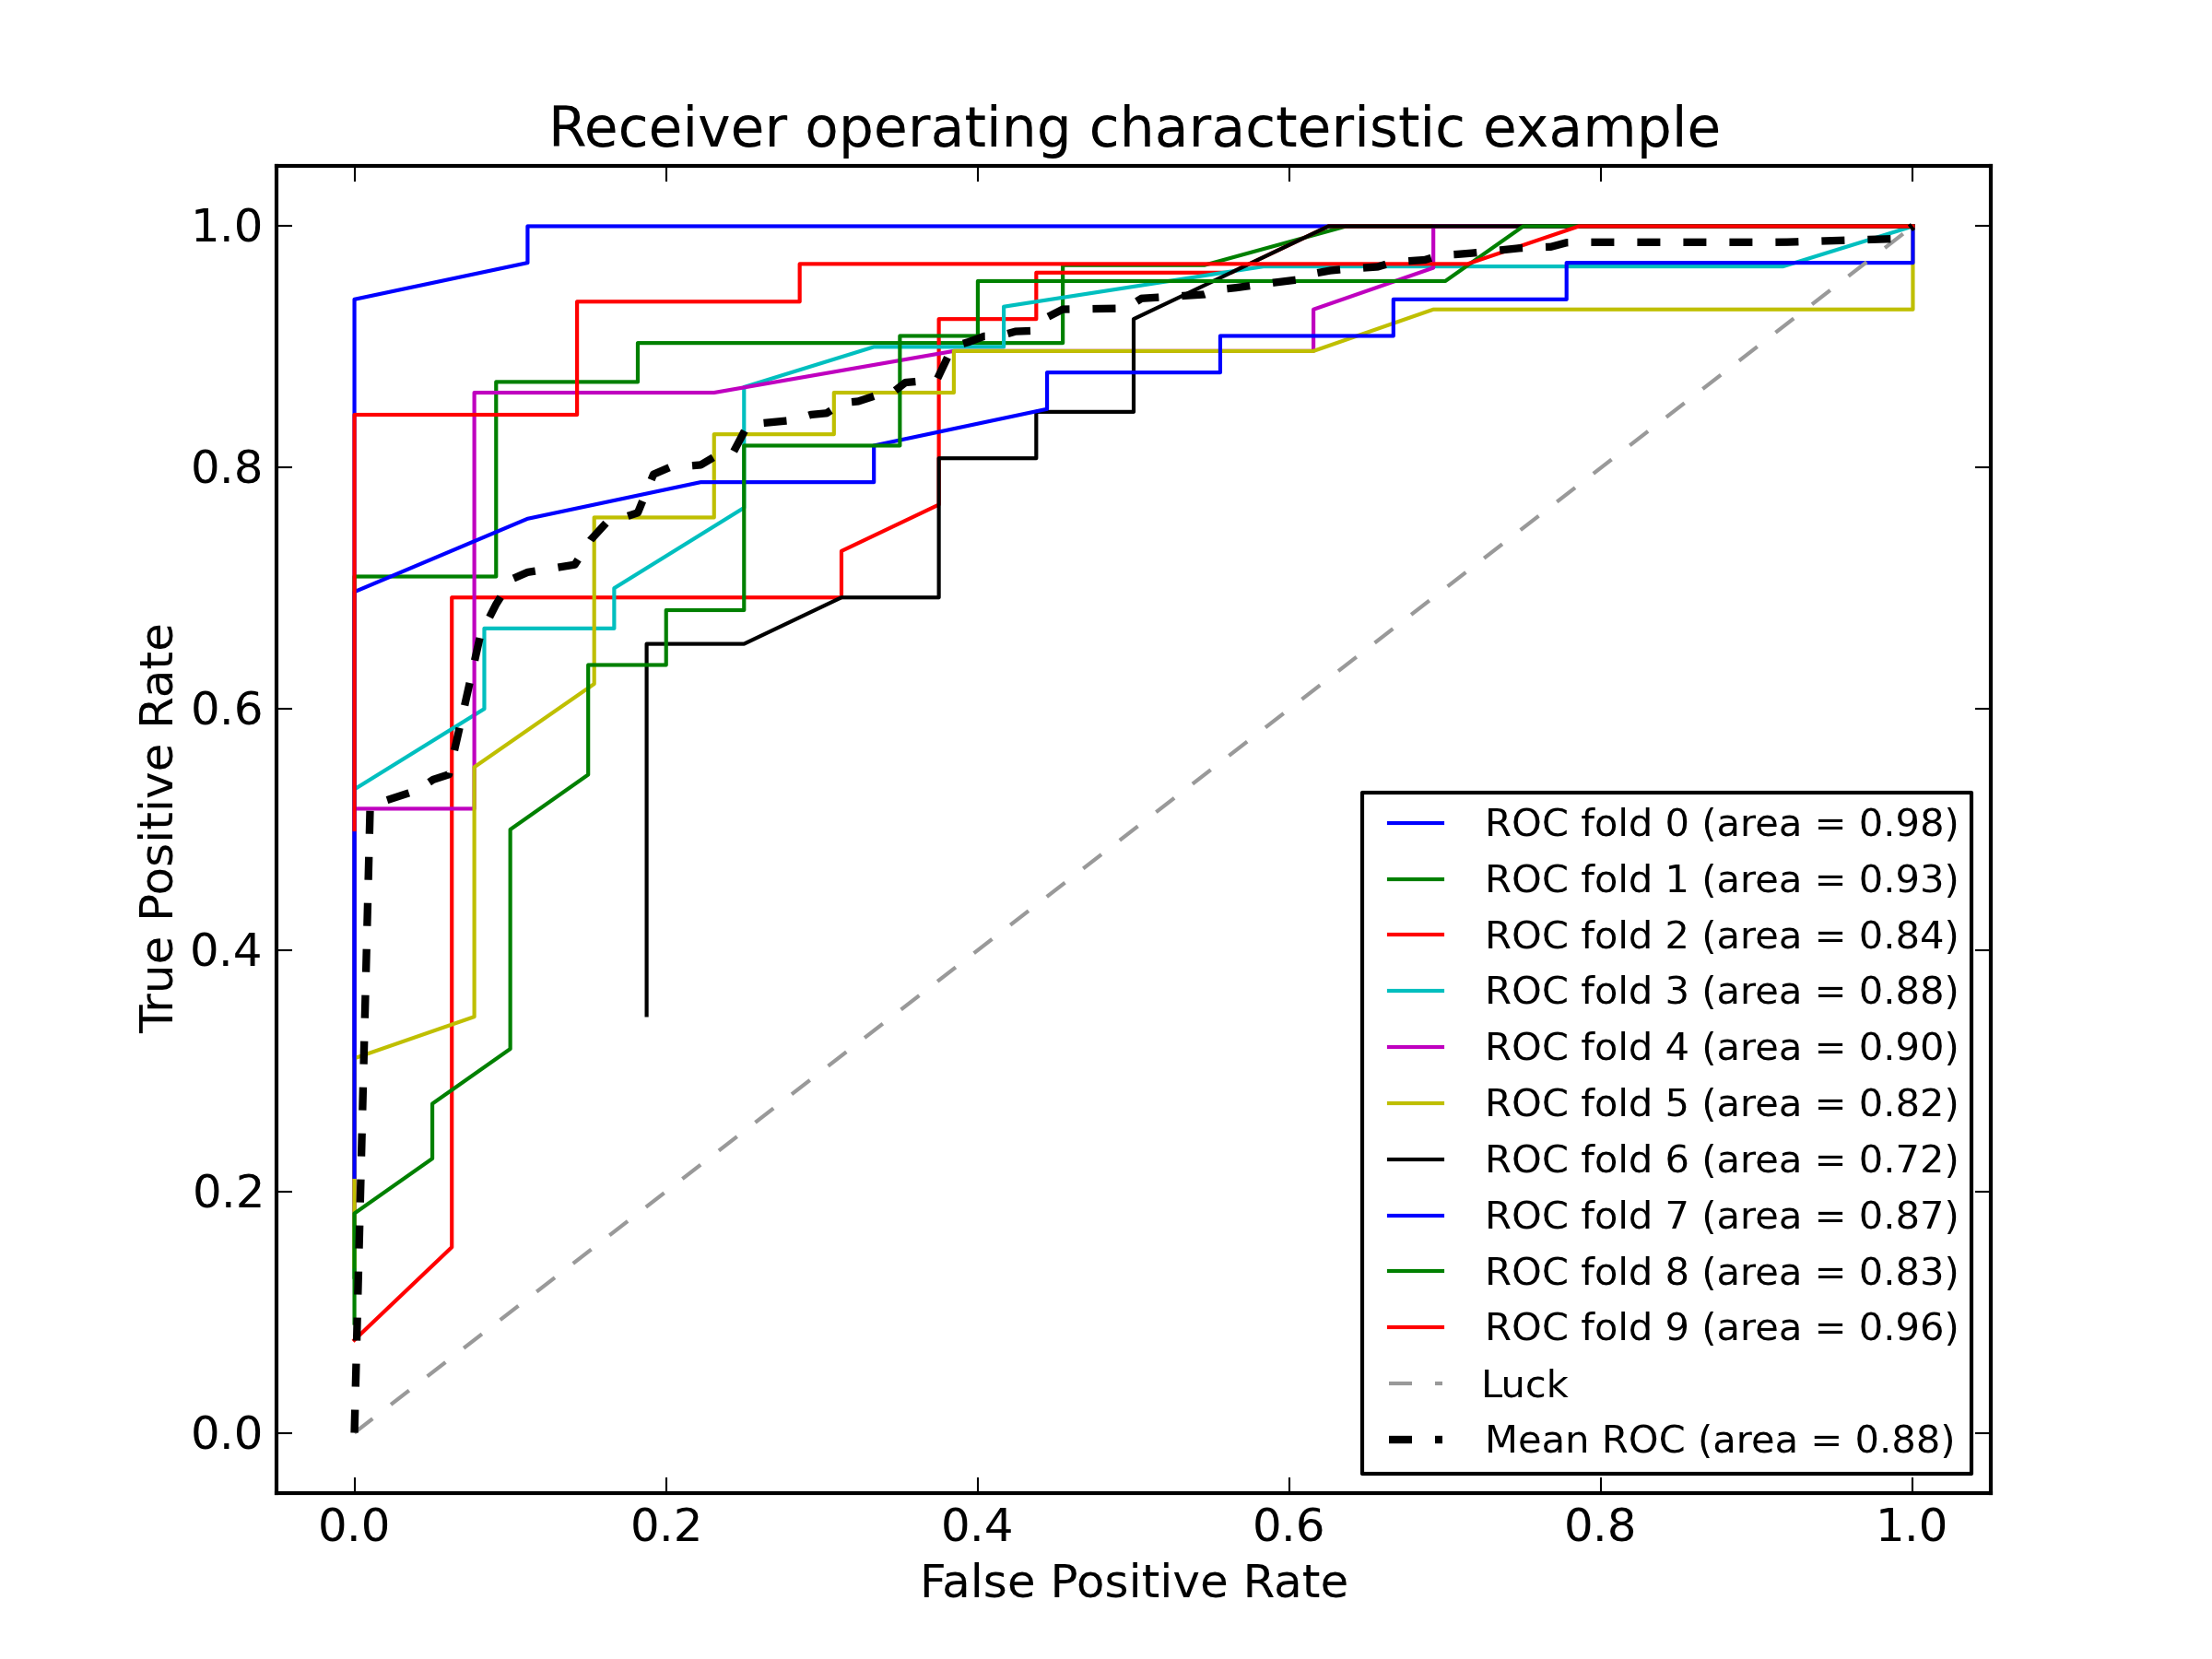
\includegraphics[width=0.36\textwidth]{pics/1_590_forest.png}}
\quad
\subfloat[Stacking - Logistic Regression]{
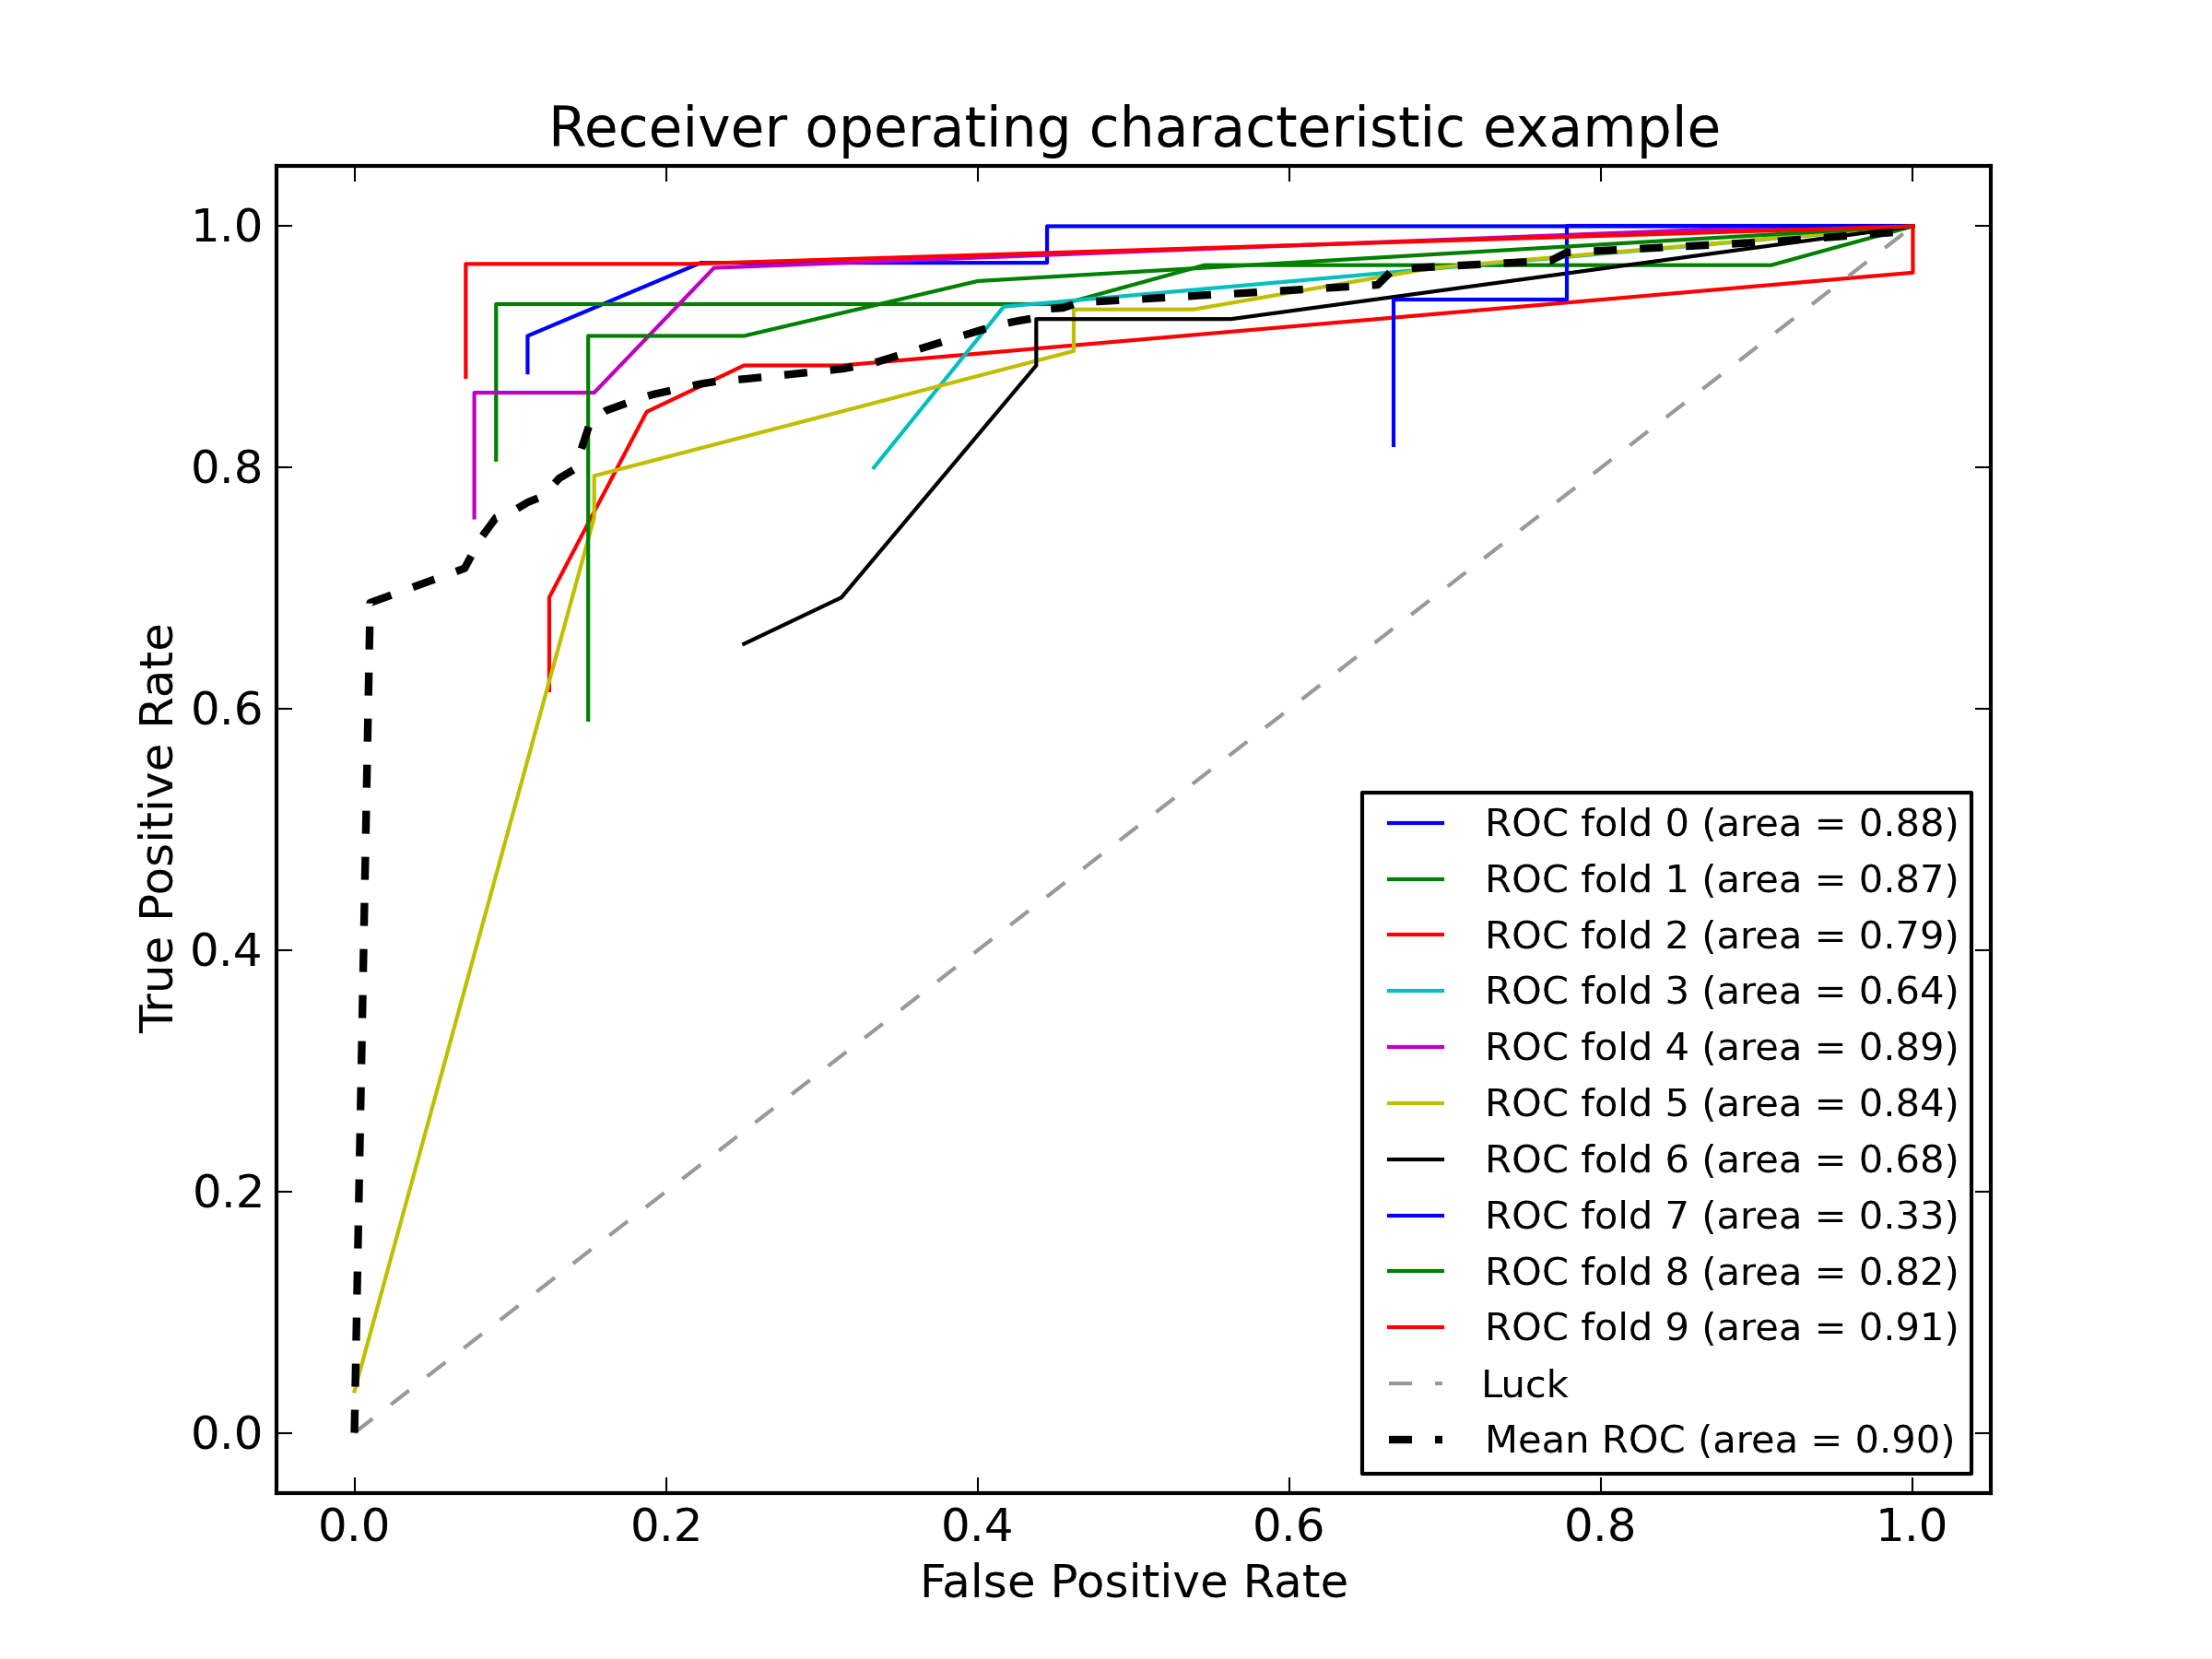
\includegraphics[width=0.36\textwidth]{pics/1_590_wmm.png}}
\quad
\subfloat[Stacking - Multi-Response Linear Models]{
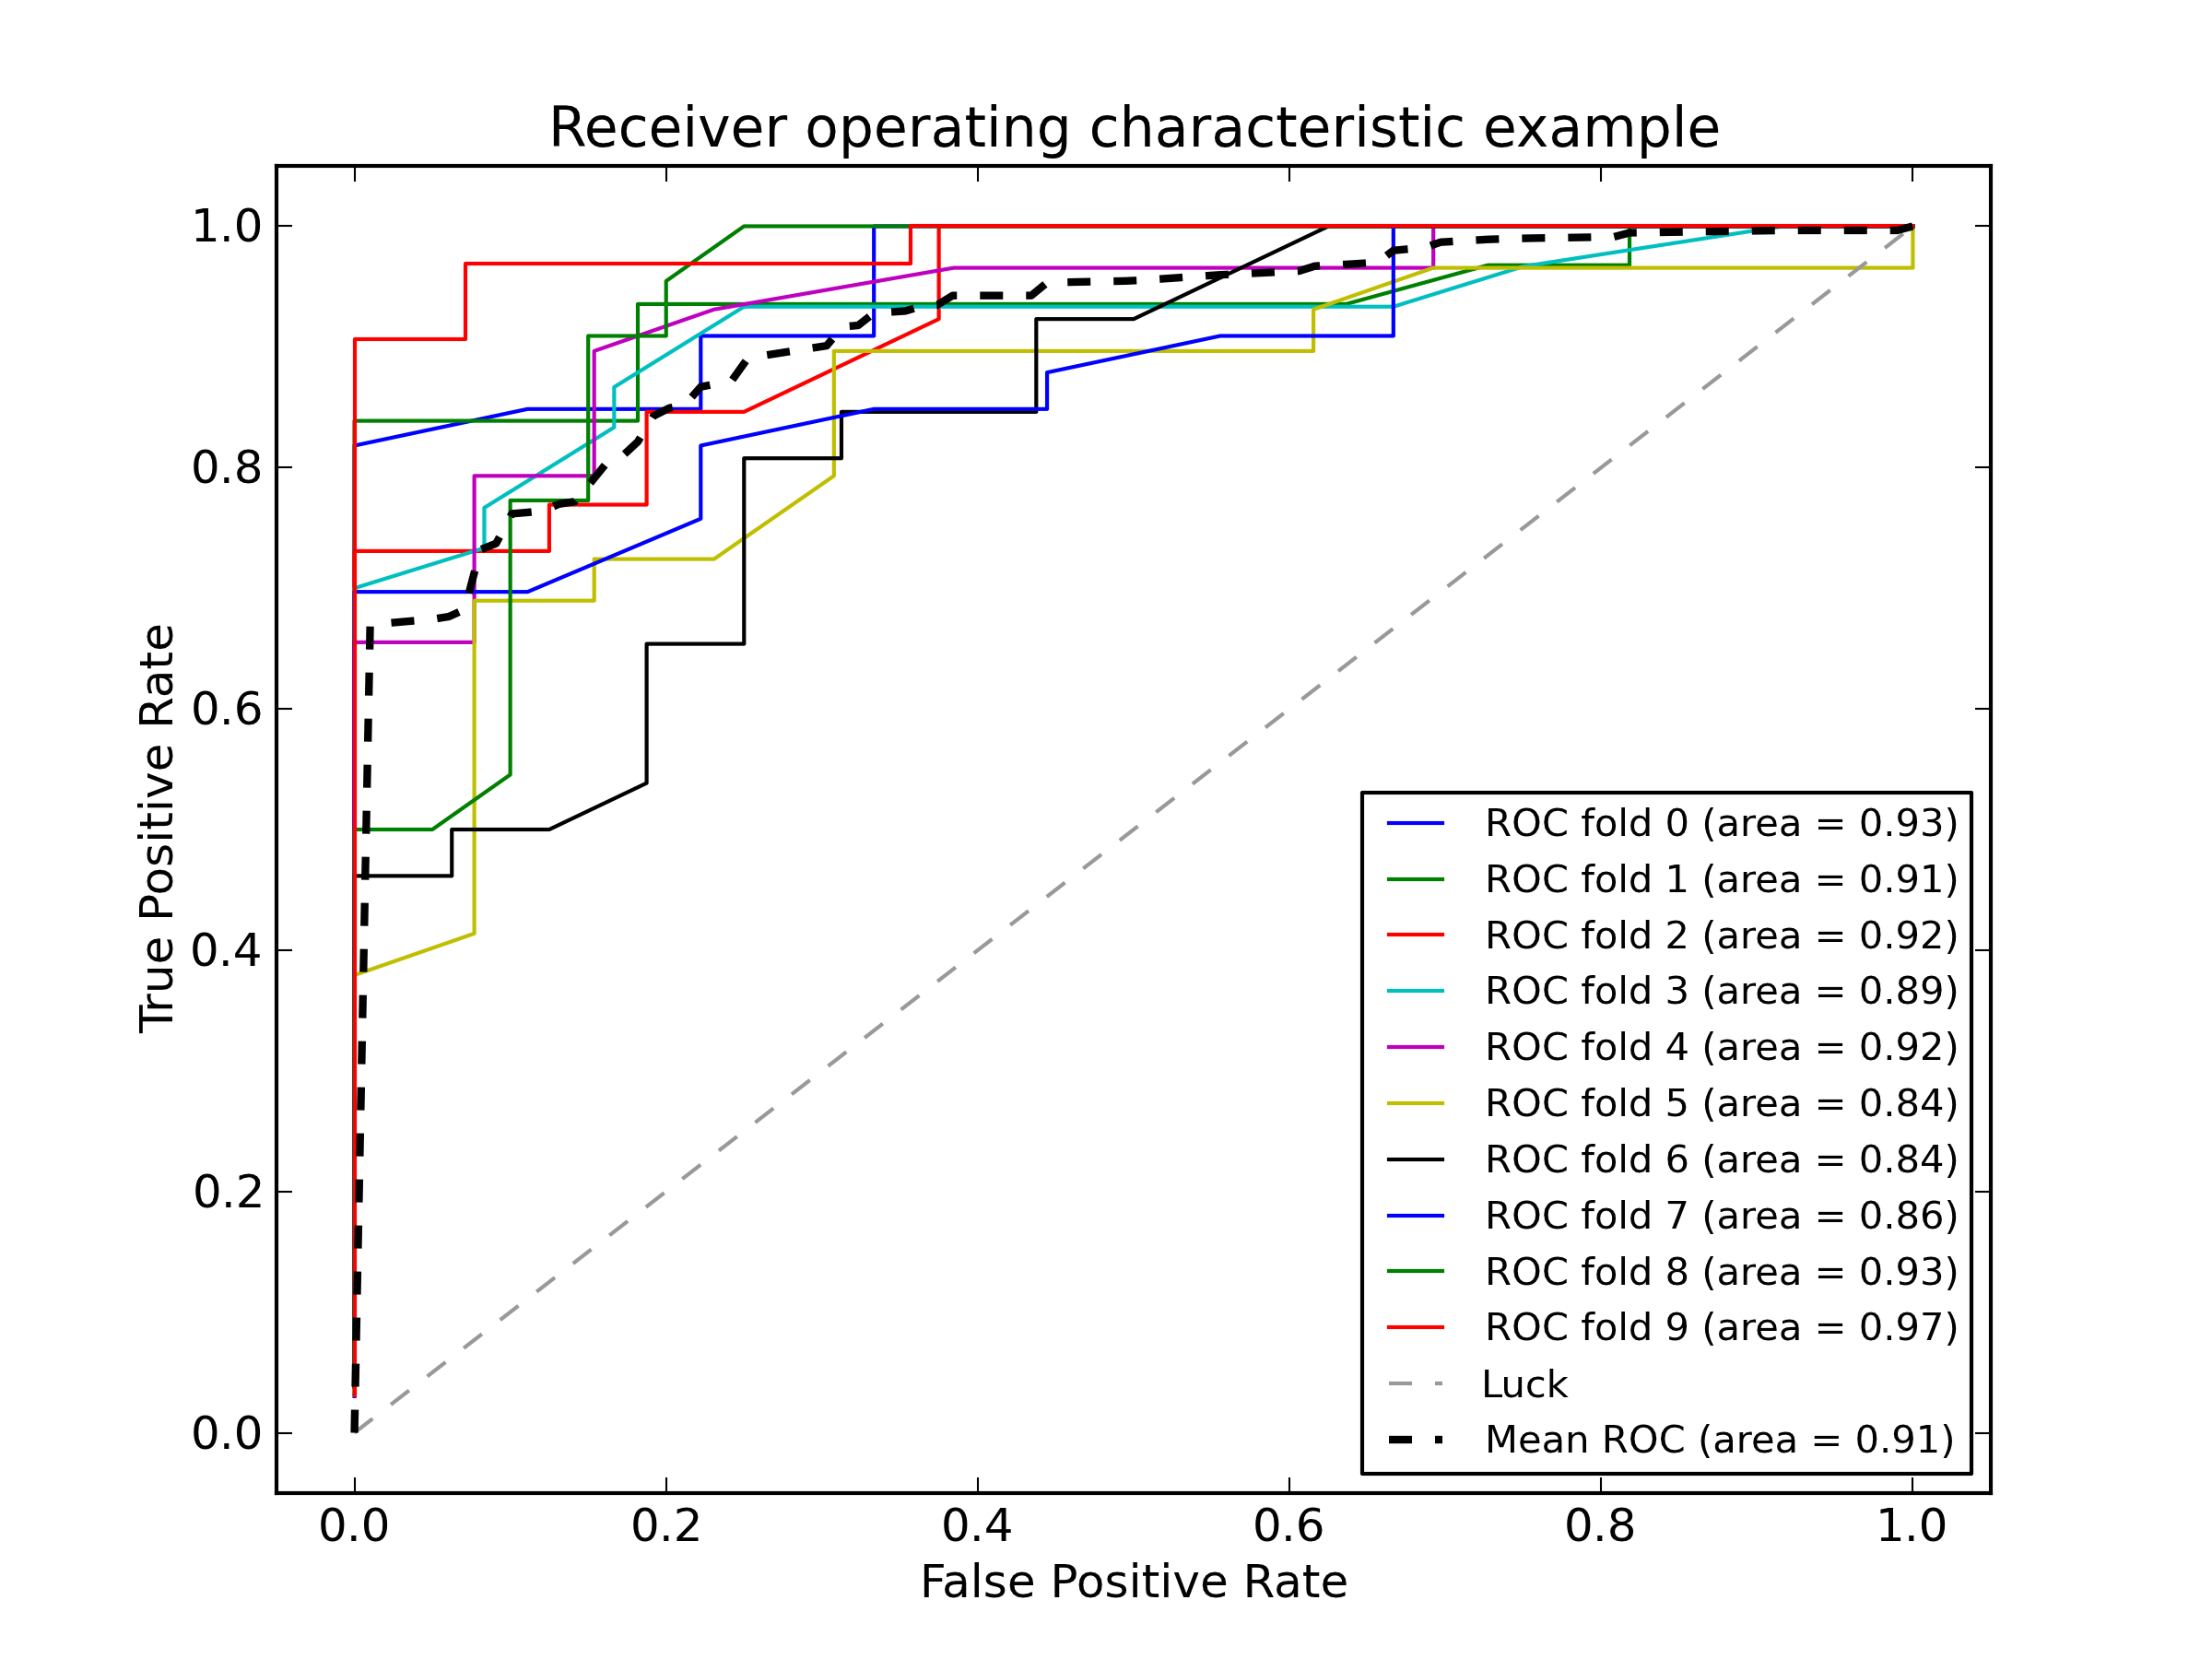
\includegraphics[width=0.36\textwidth]{pics/1_590_smm.png}}
\caption{Results for Features 1-8}
\label{fig:fig2}
\end{figure}

\begin{figure}[t]
\centering
\subfloat[Logistic Regression]{
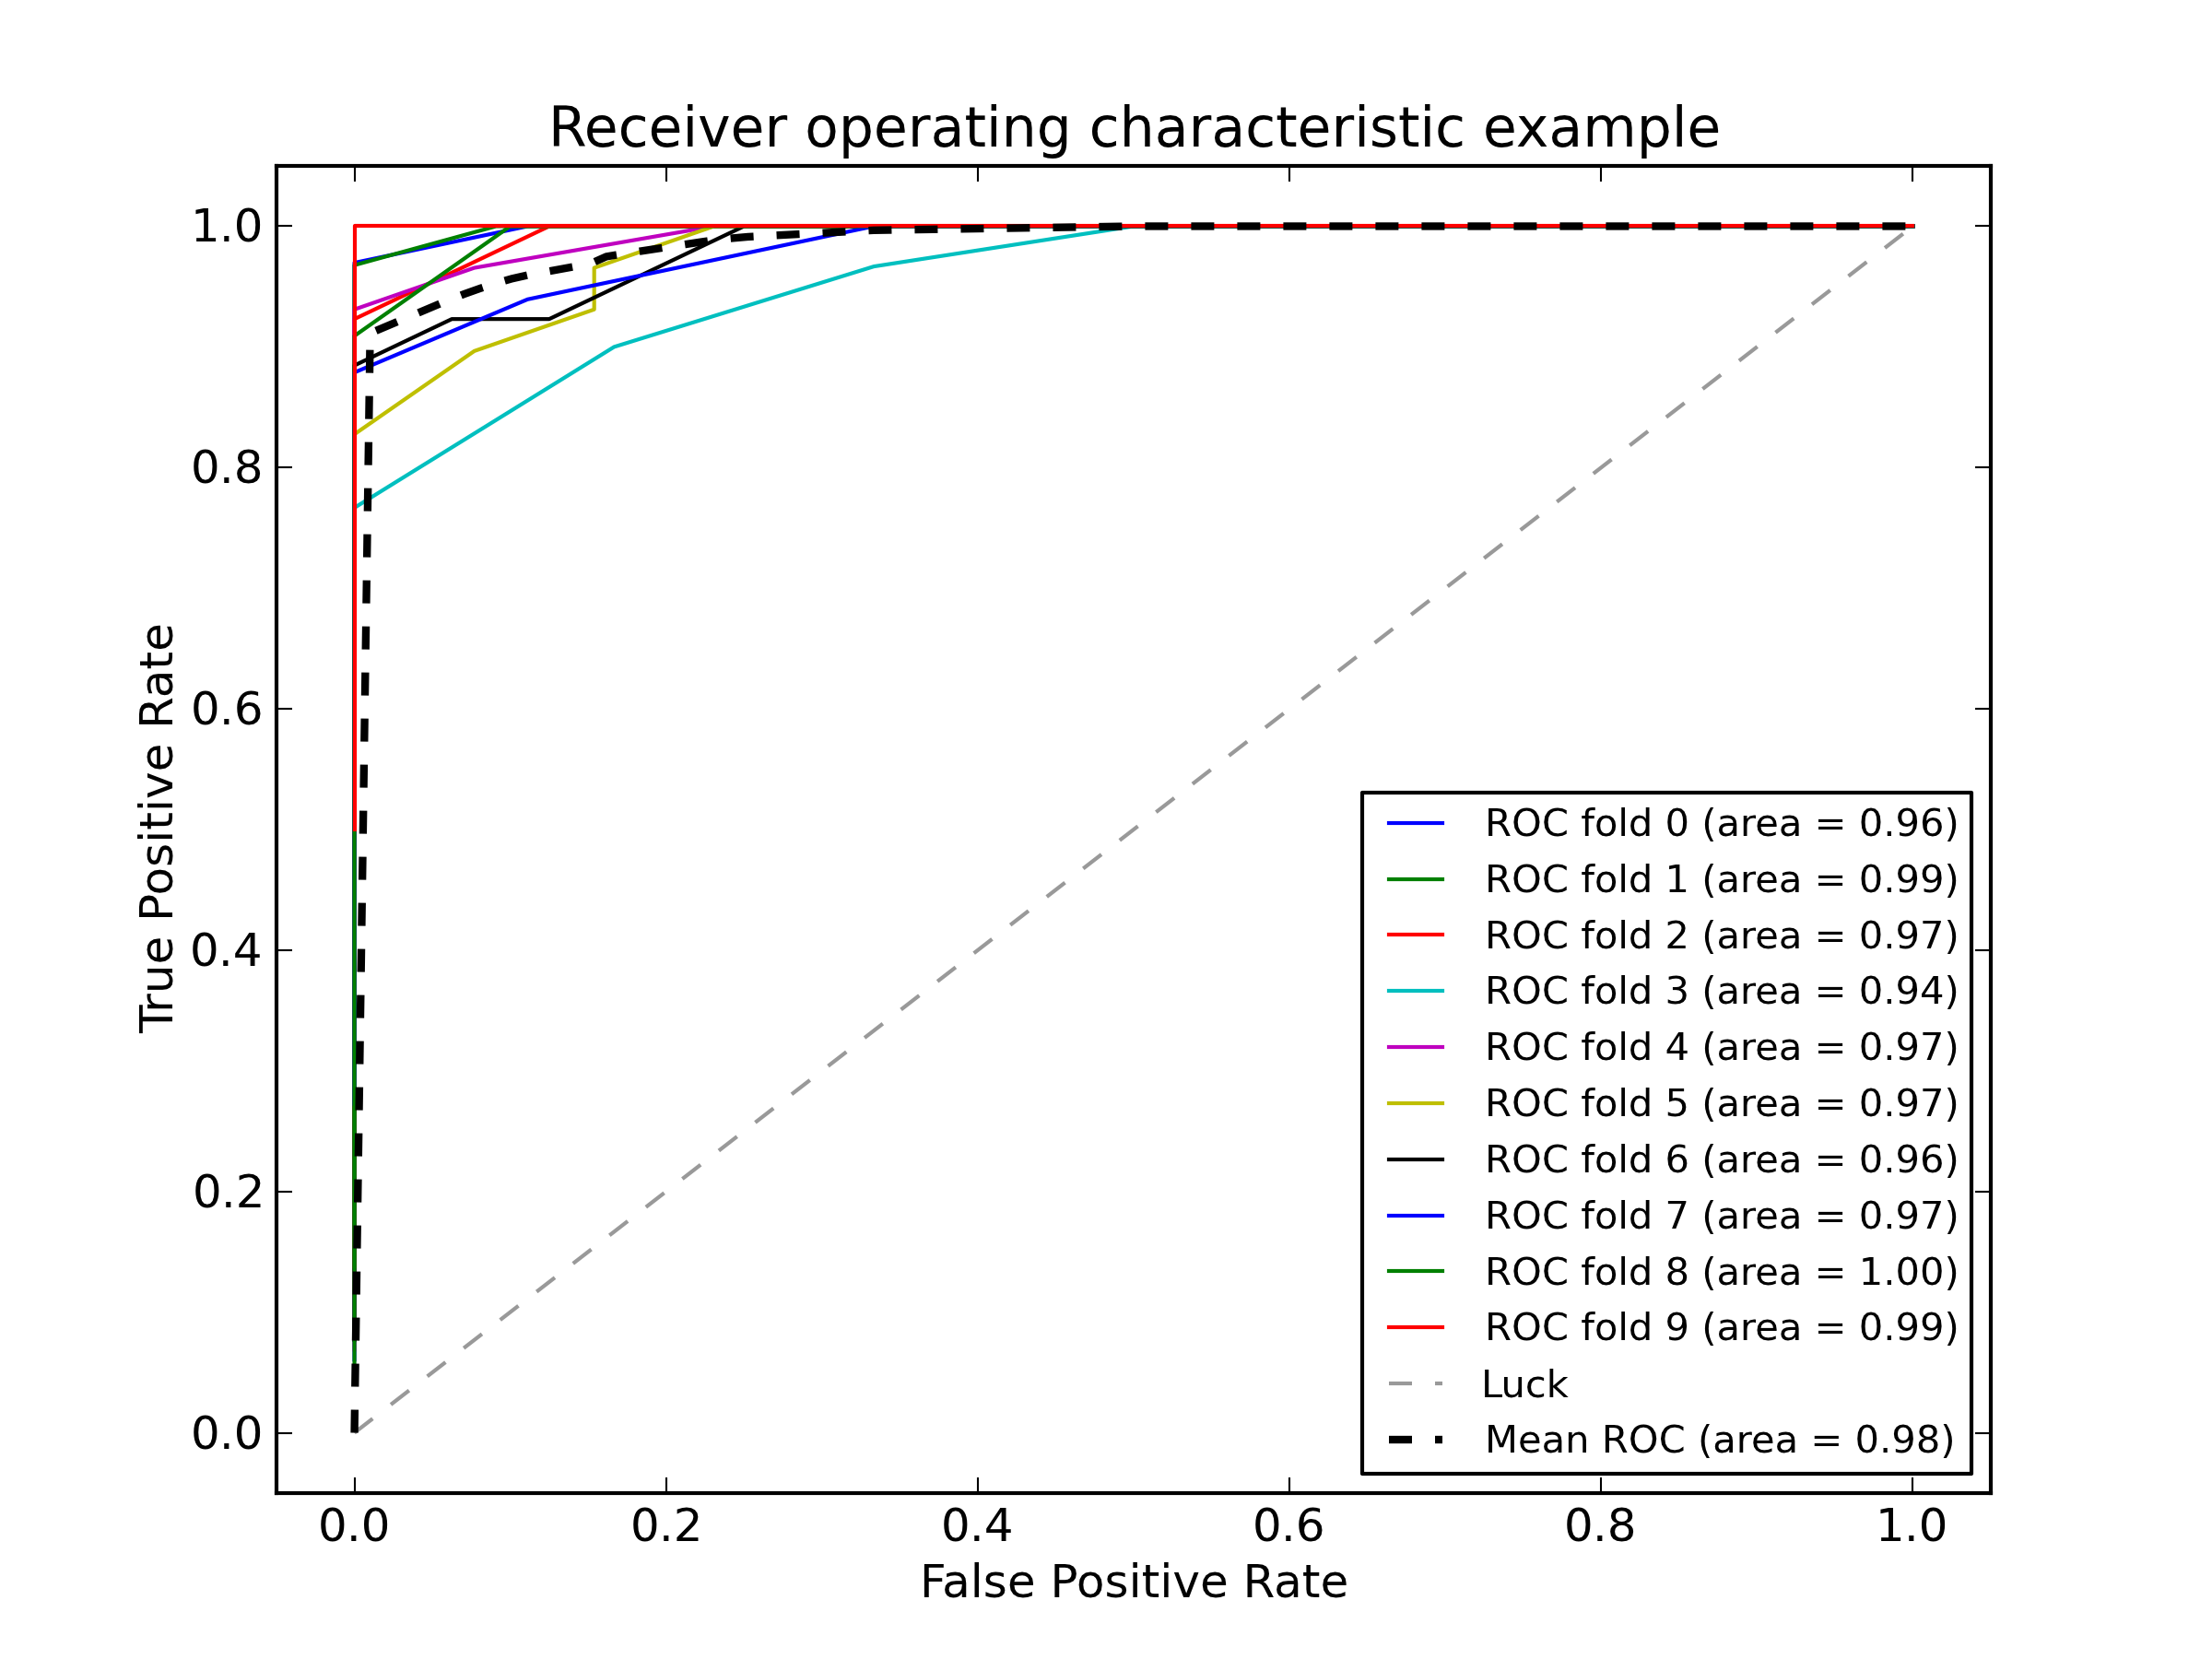
\includegraphics[width=0.36\textwidth]{pics/2_590_logit.png}}
\quad
\subfloat[Decision Trees]{
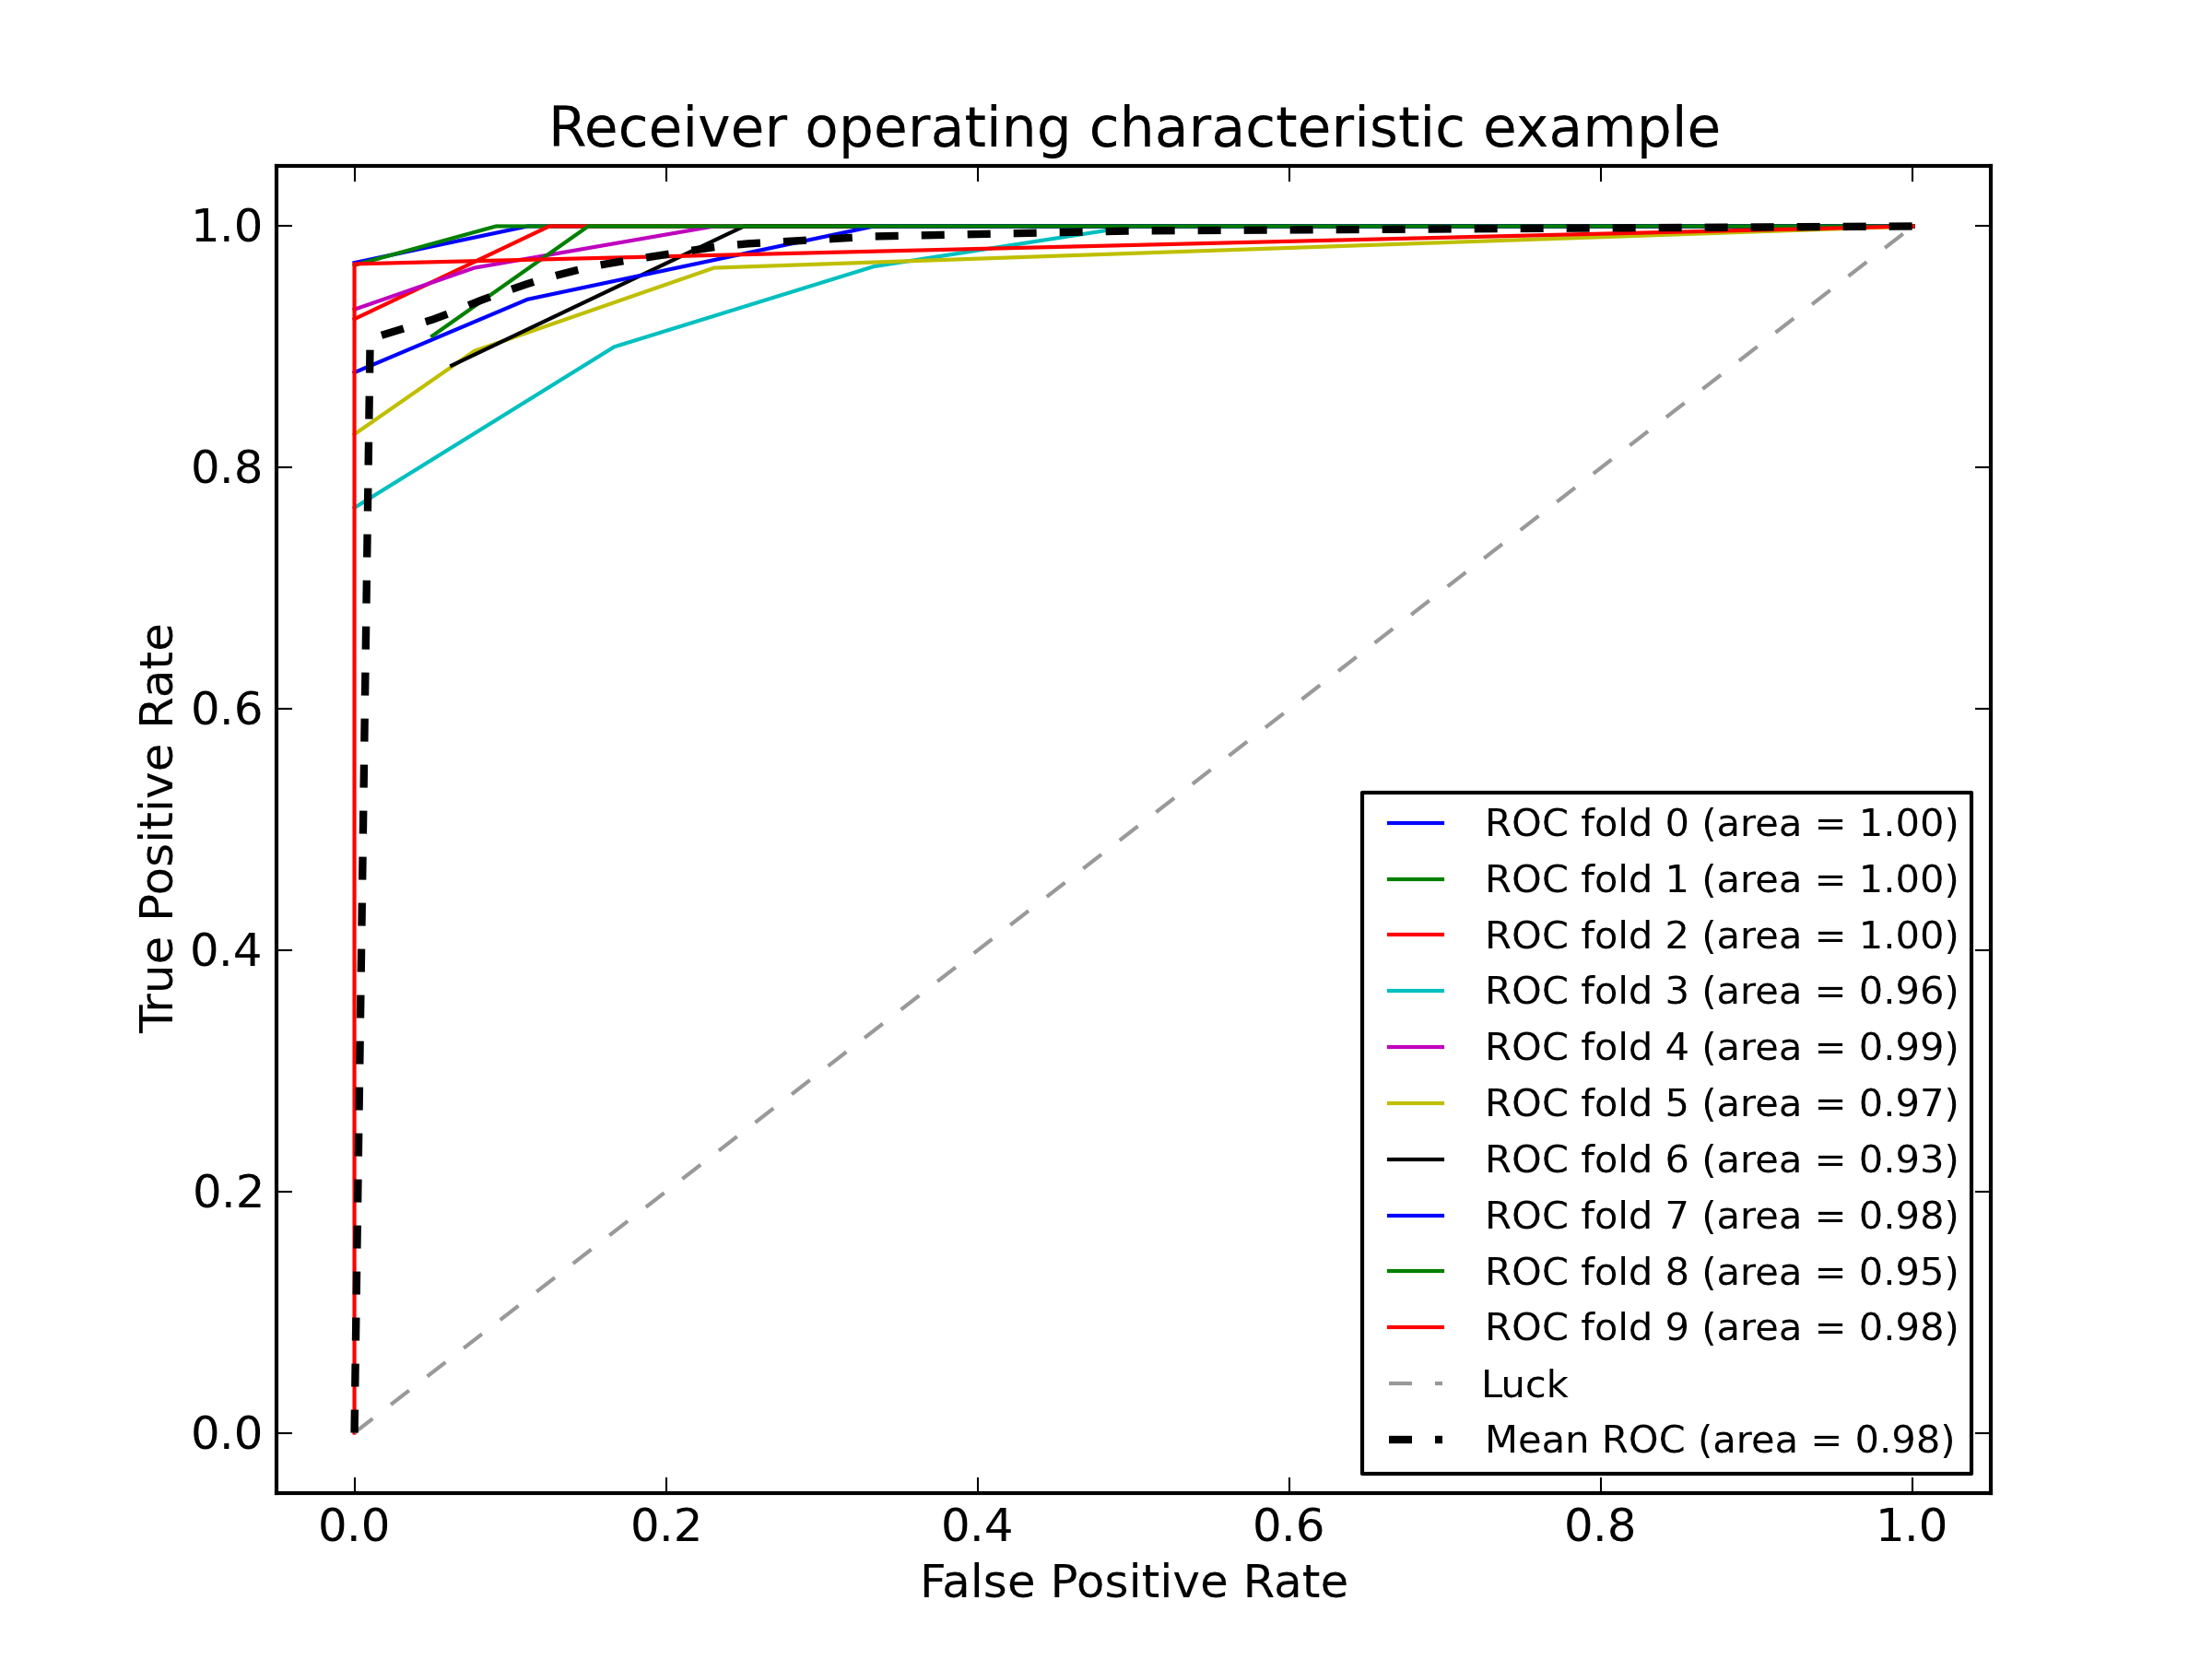
\includegraphics[width=0.36\textwidth]{pics/2_590_dtree.png}}
\quad
\subfloat[Multinomial Bayes]{
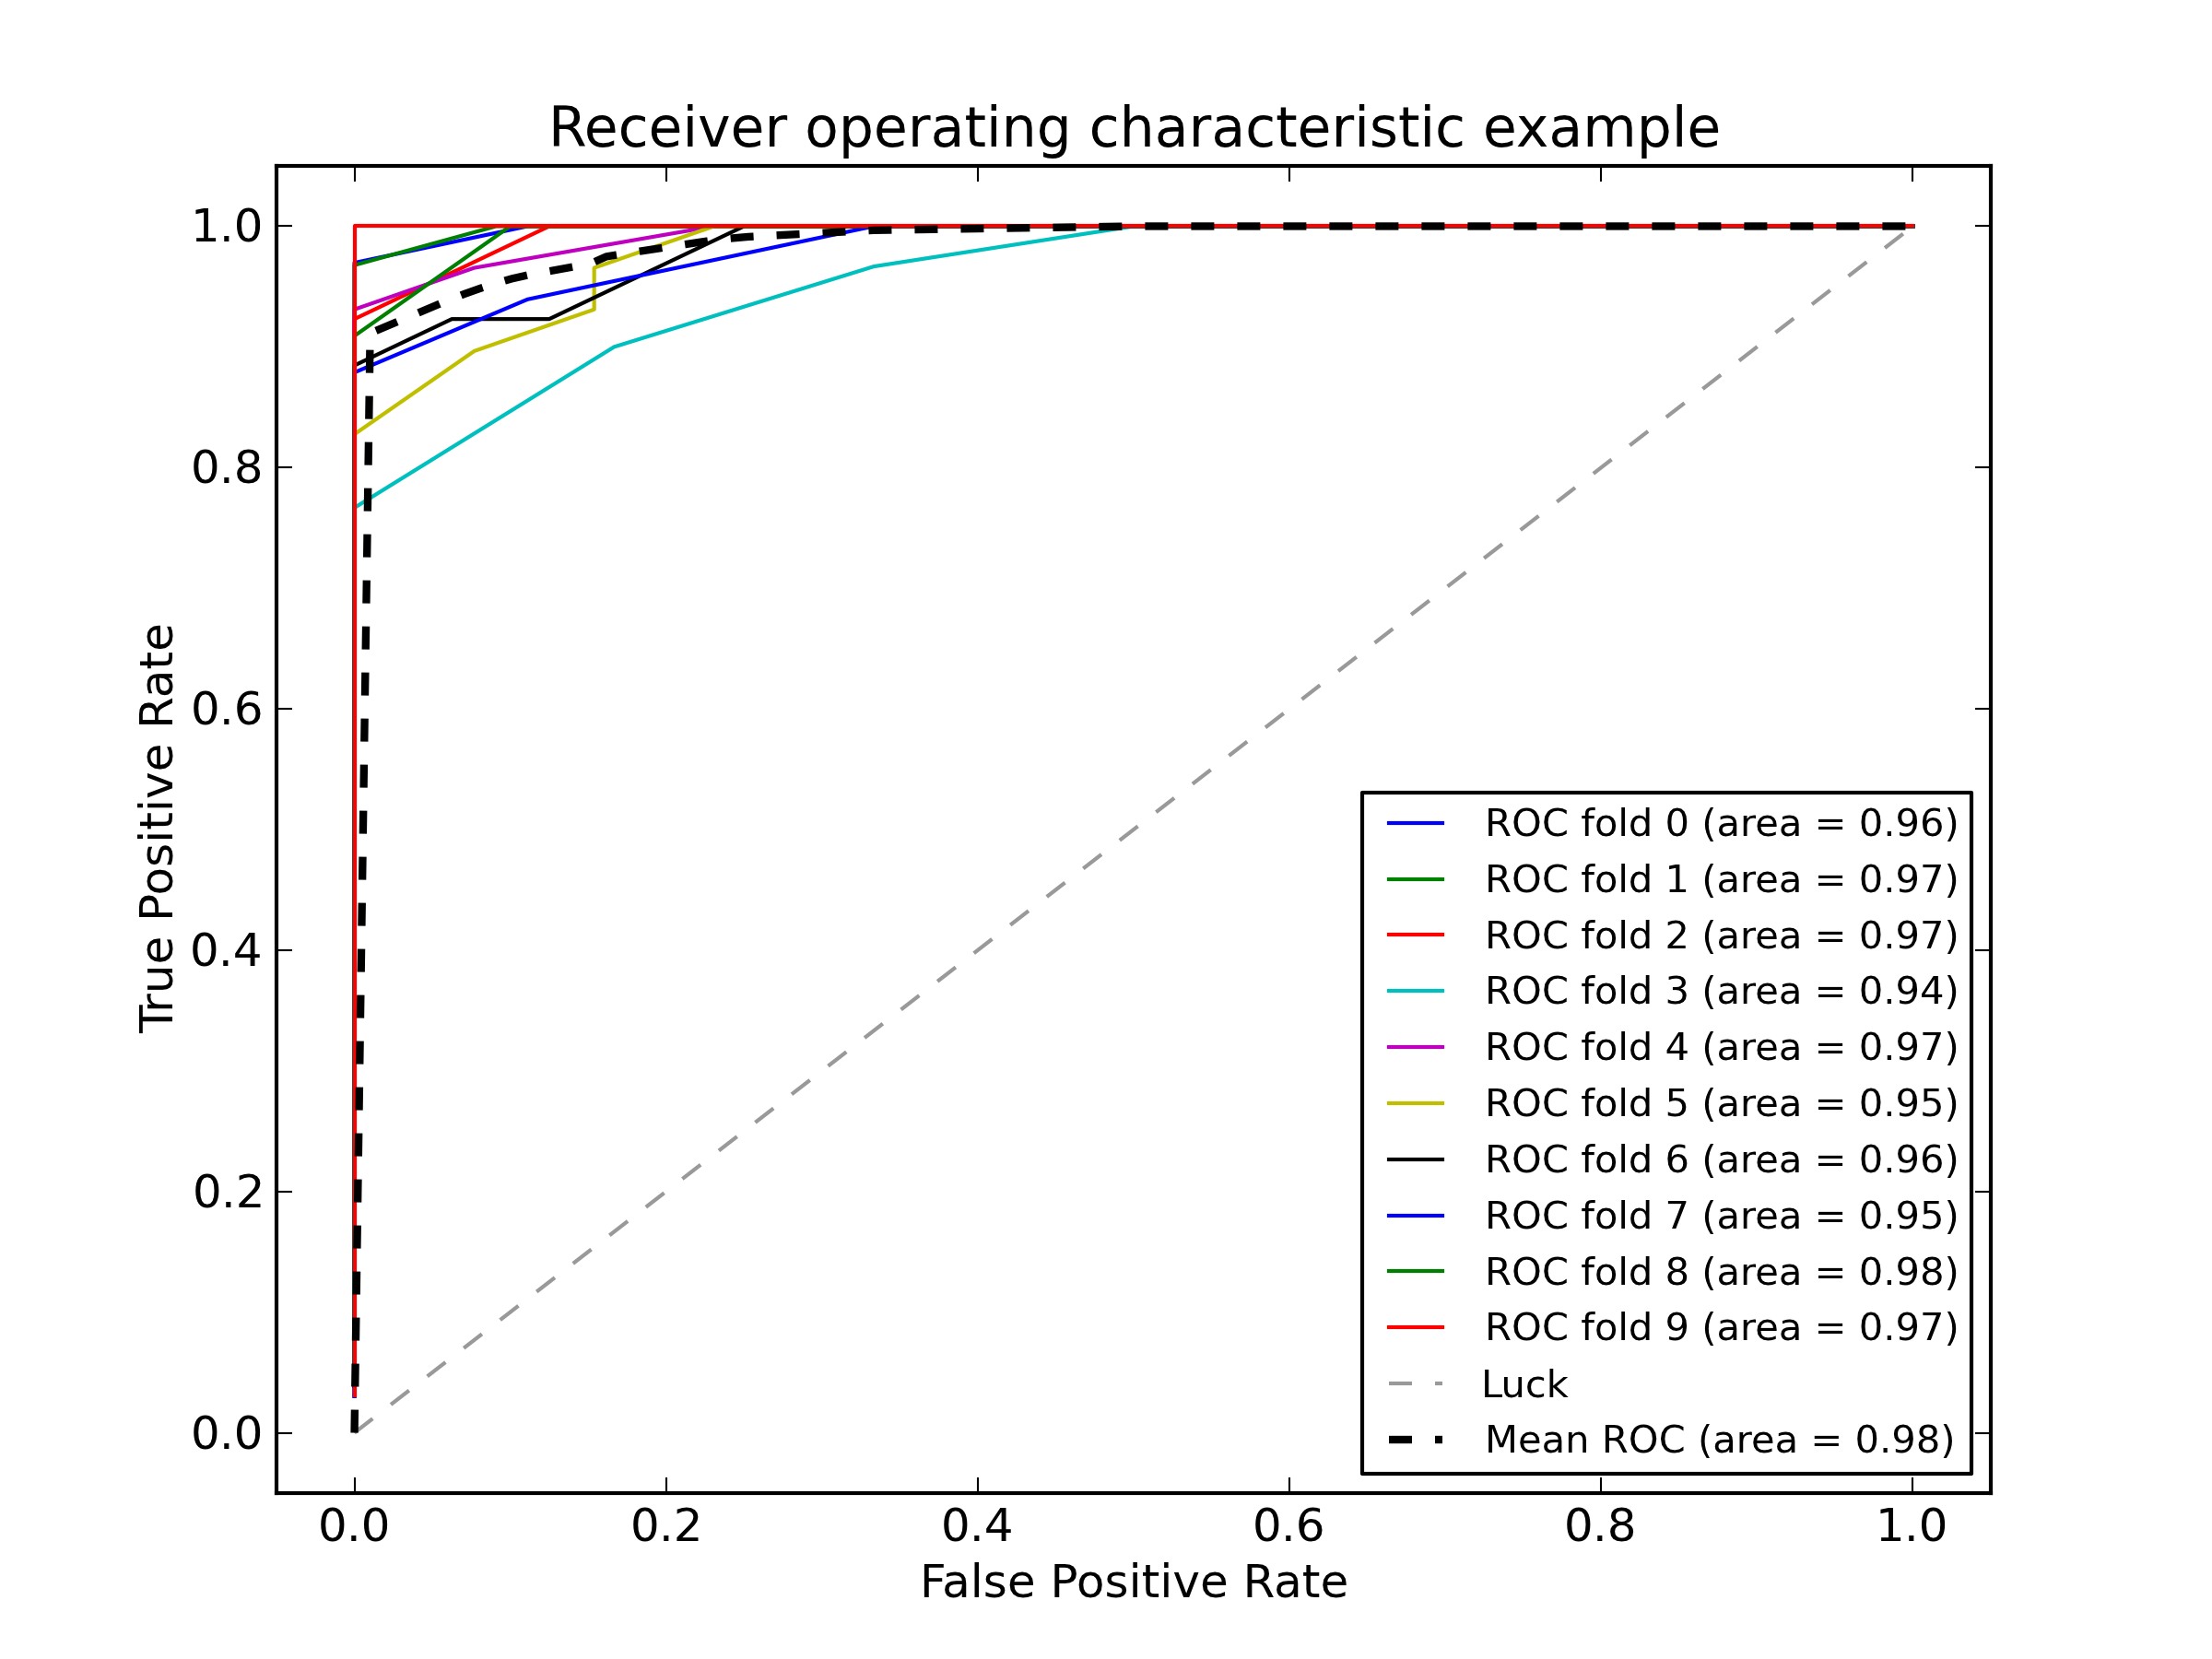
\includegraphics[width=0.36\textwidth]{pics/2_590_multi.png}}
\quad
\subfloat[Support Vector Machines]{
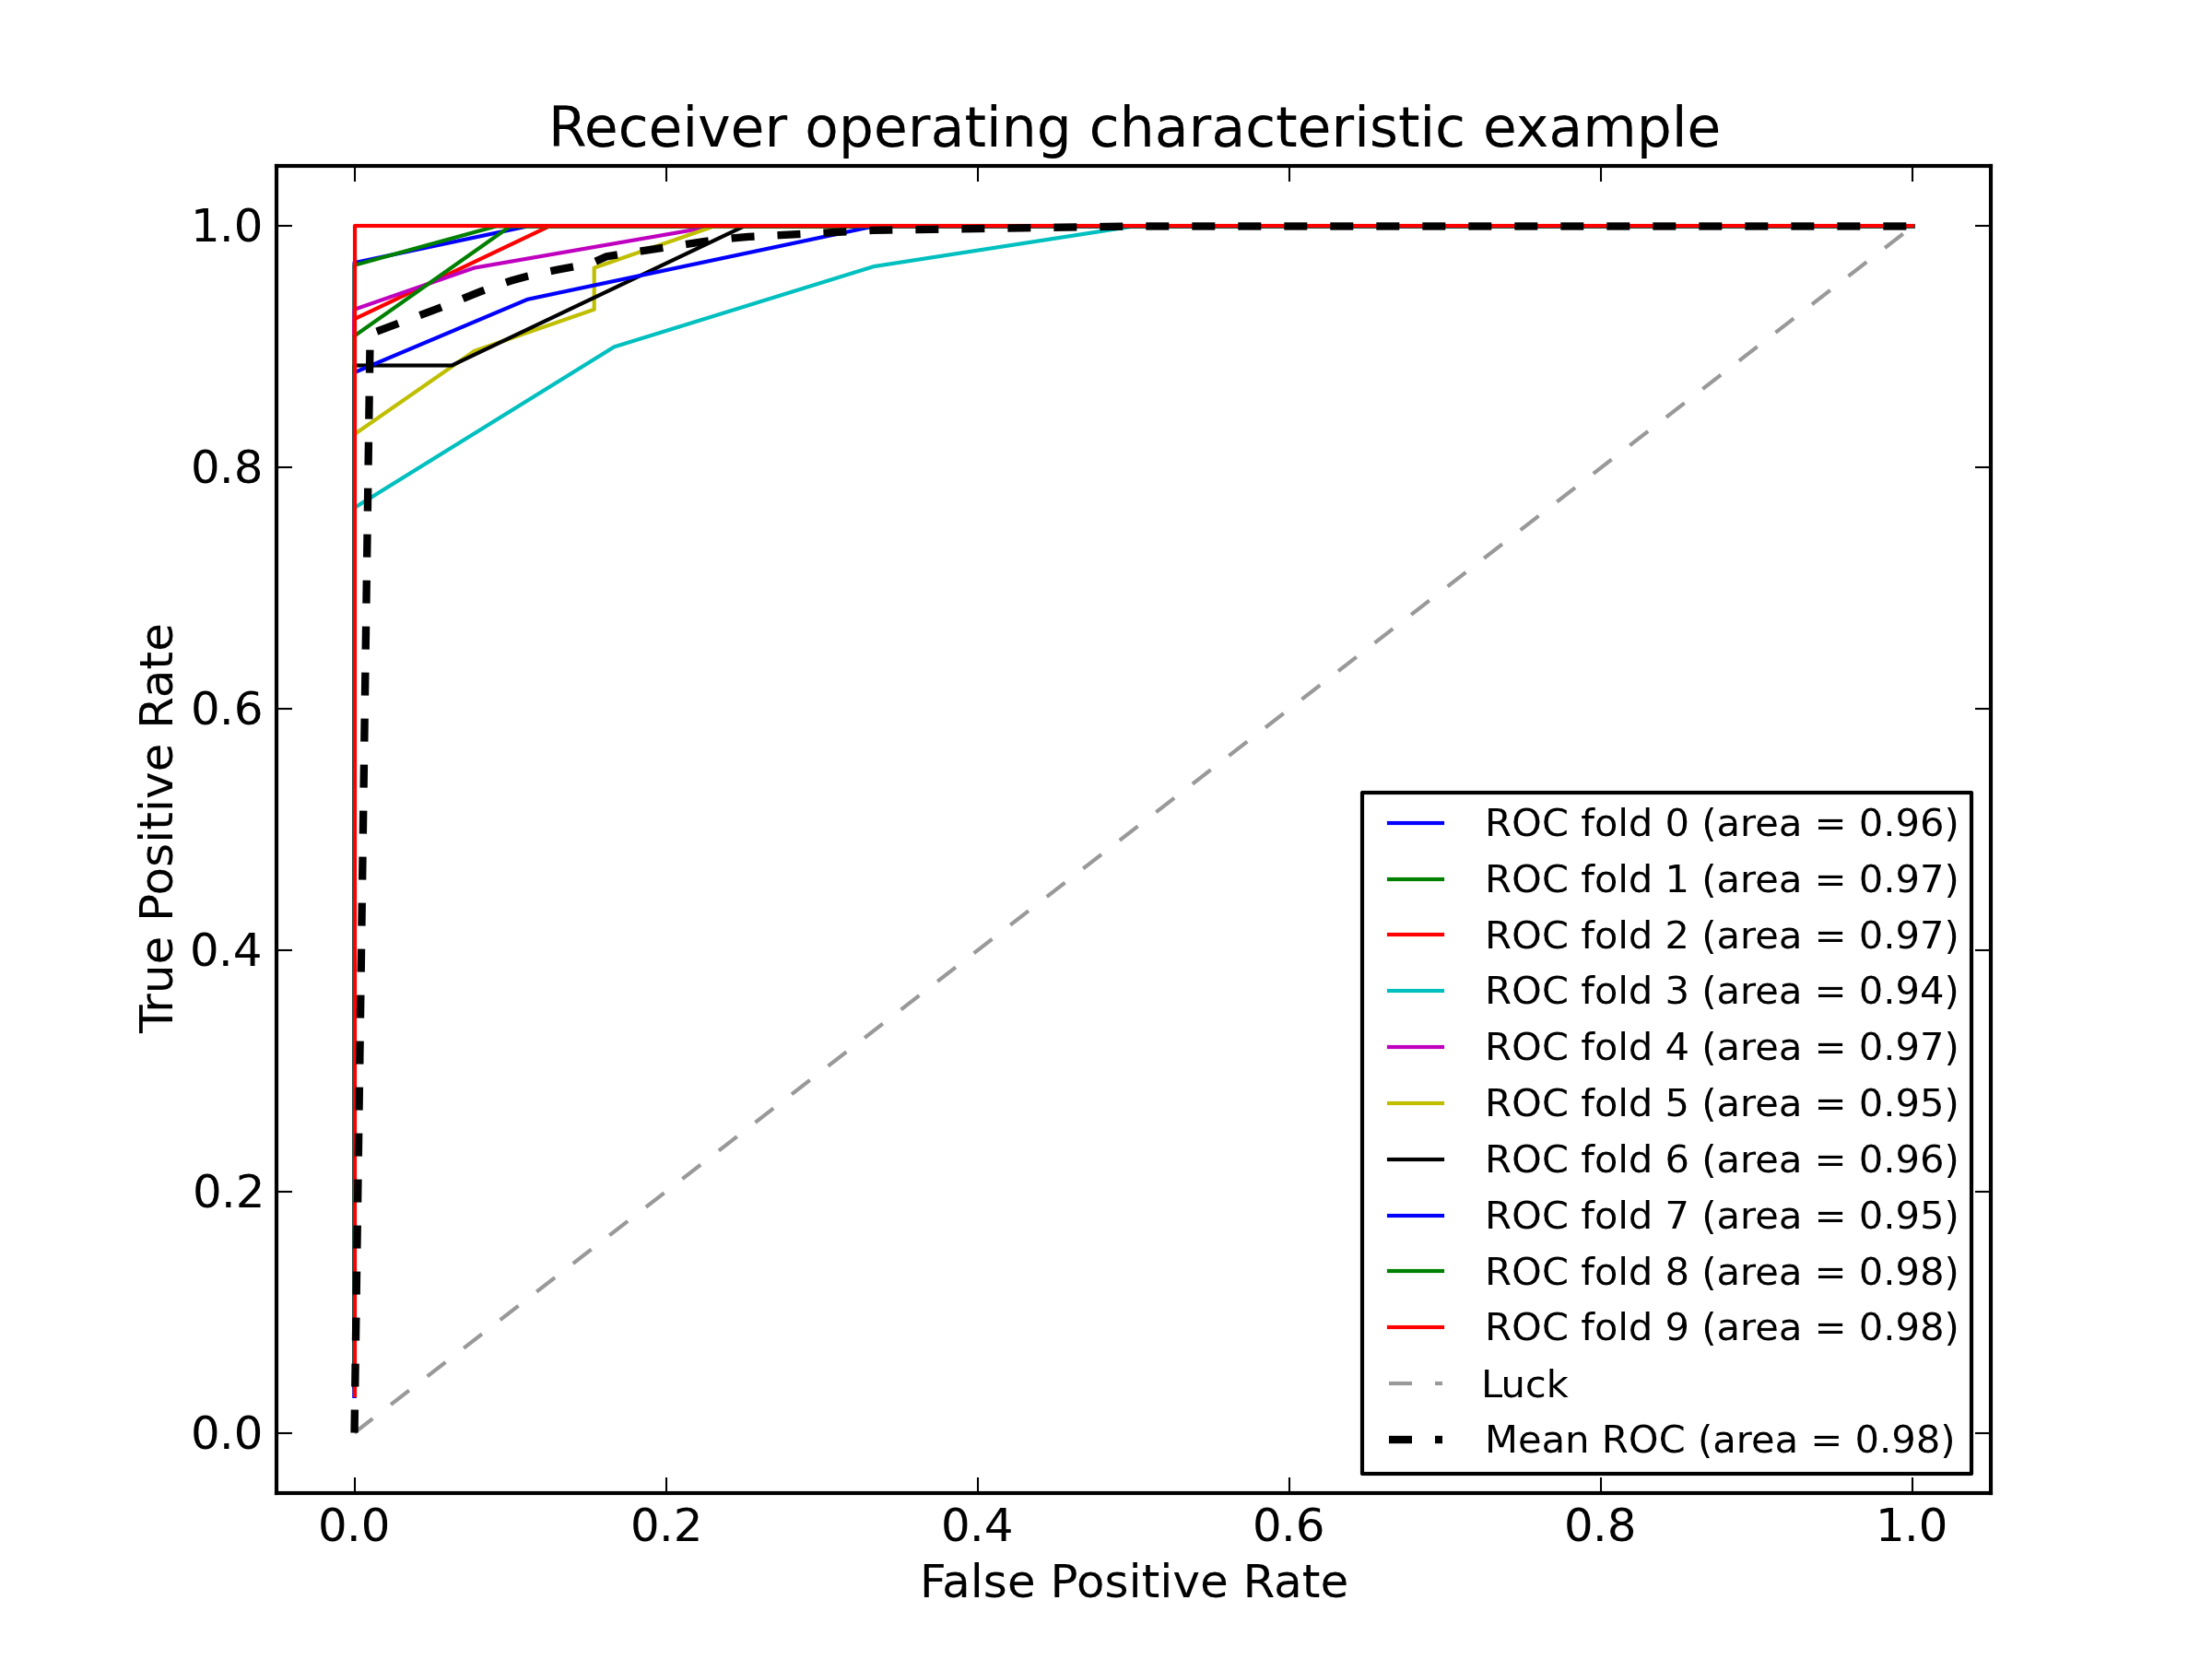
\includegraphics[width=0.36\textwidth]{pics/2_590_svm.png}}
\quad
\subfloat[Random Forests]{
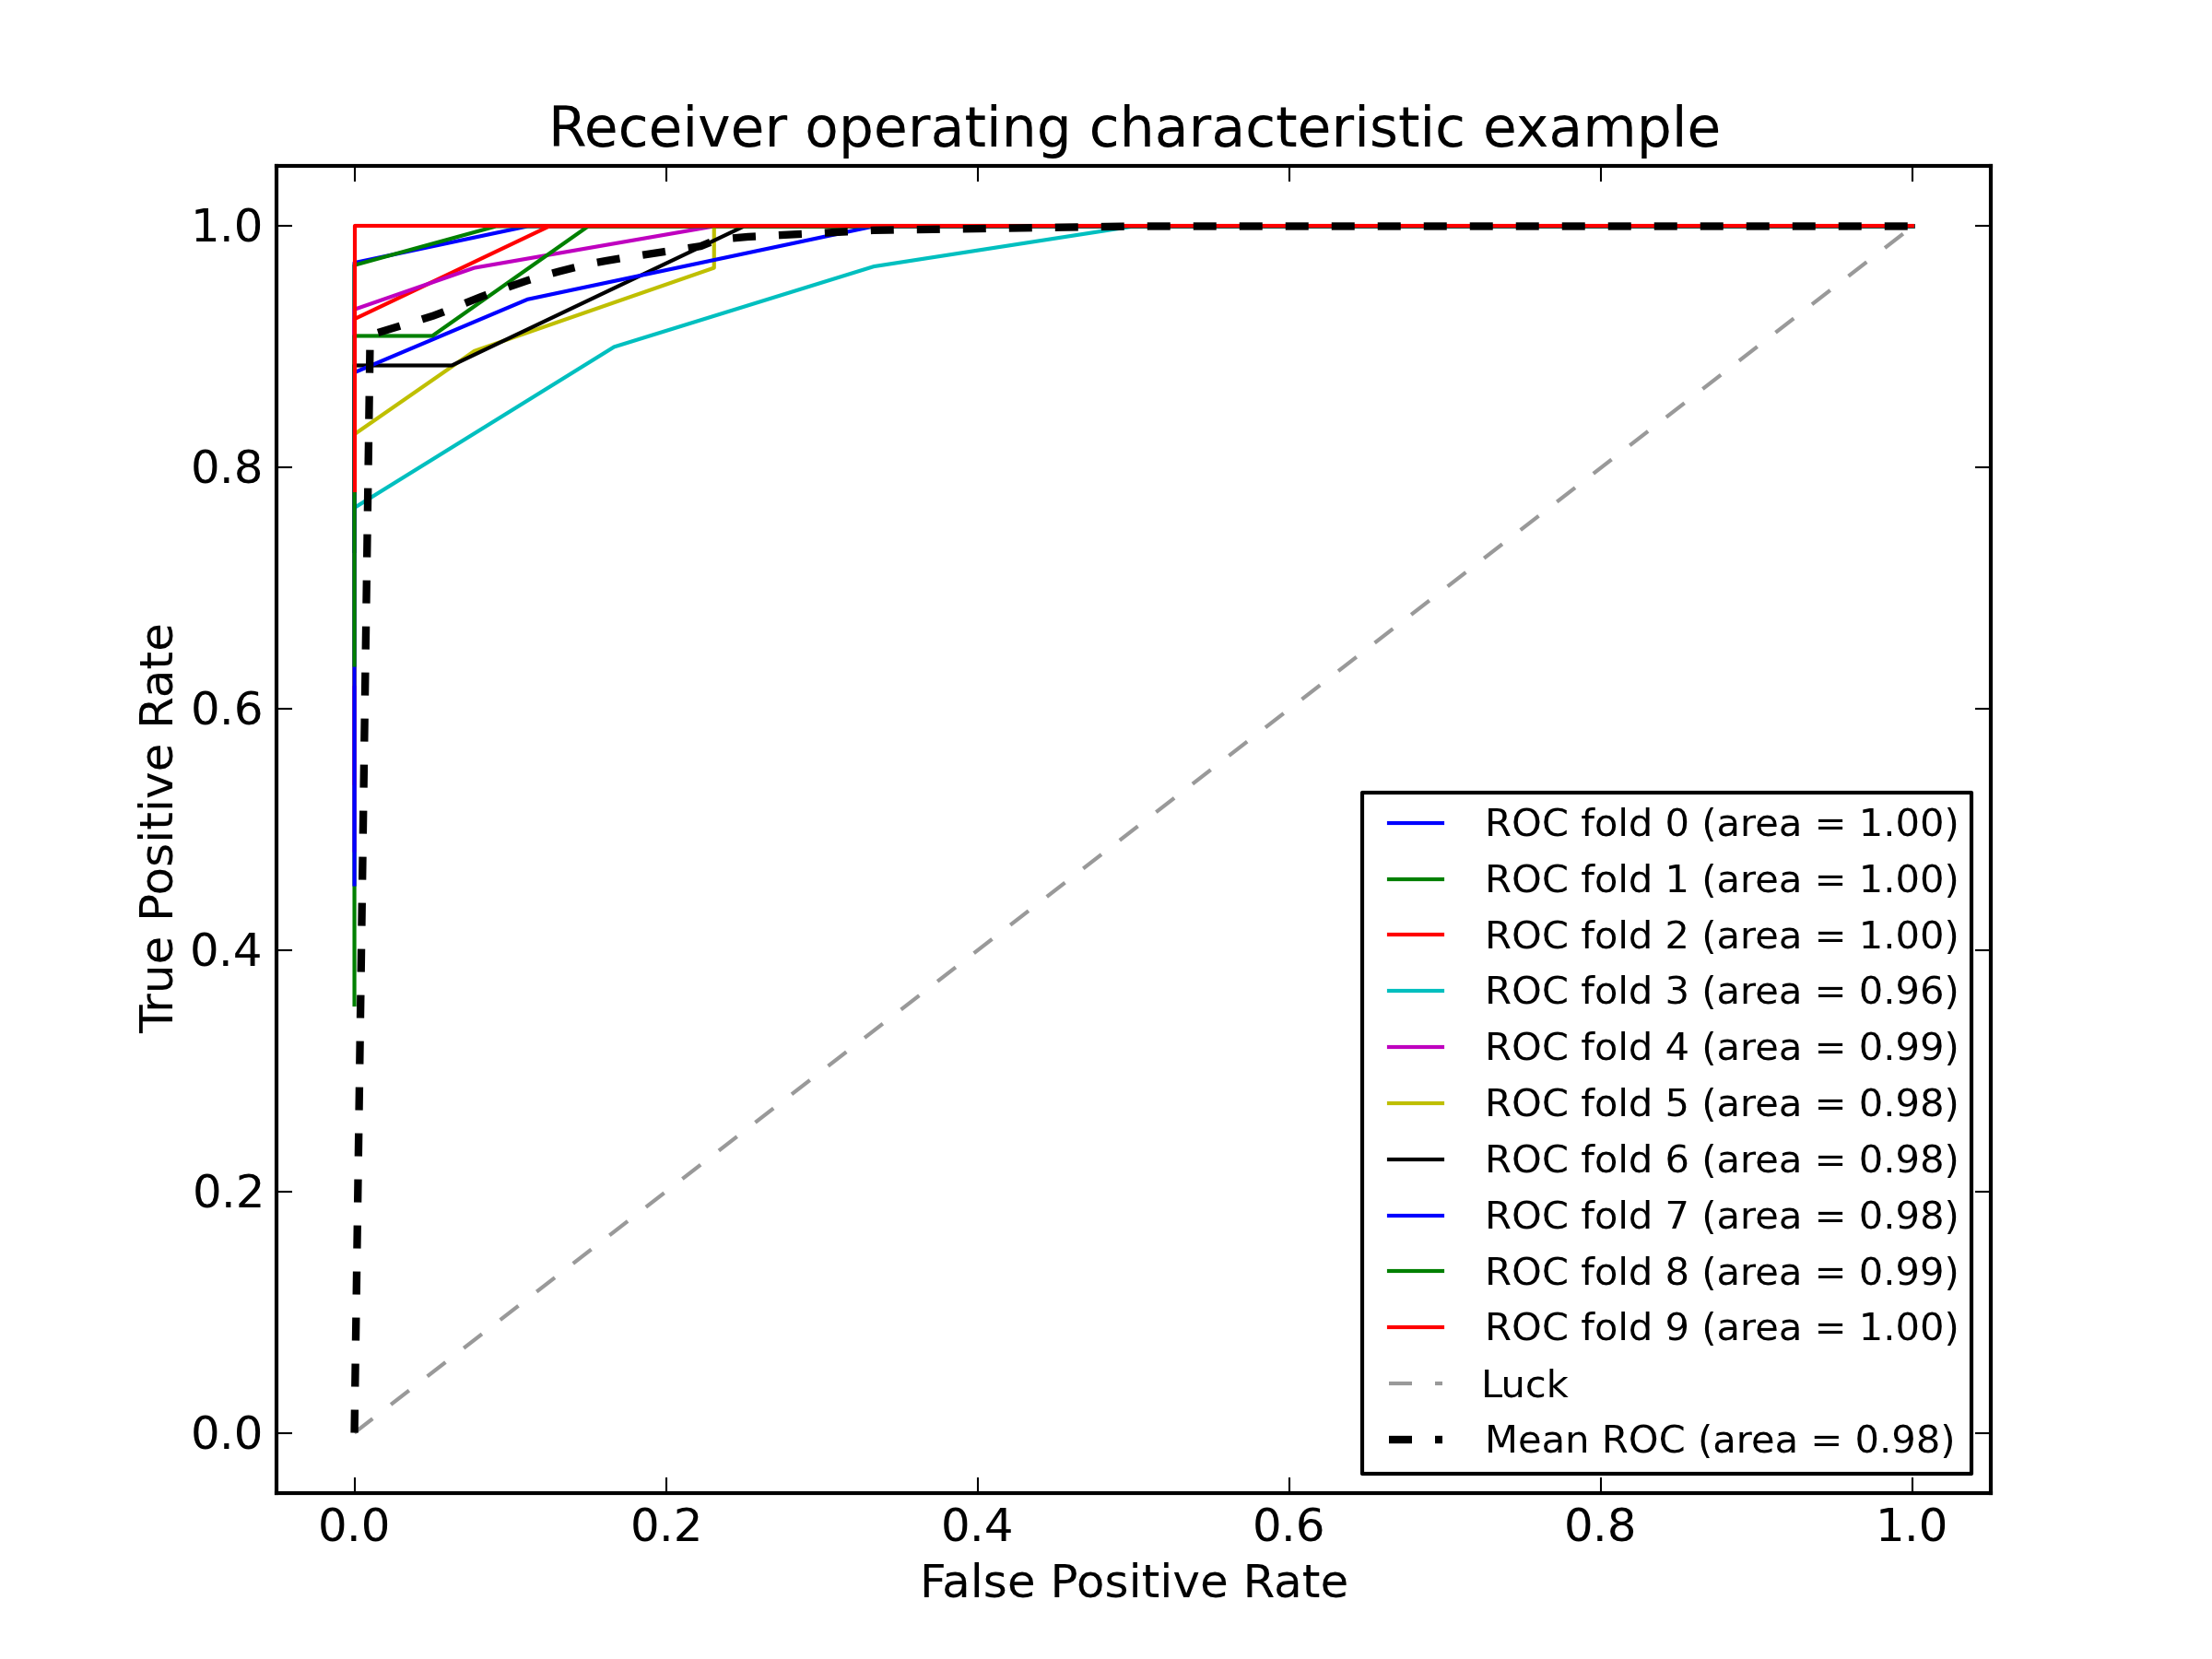
\includegraphics[width=0.36\textwidth]{pics/2_590_forest.png}}
\quad
\subfloat[Stacking - Logistic Regression]{
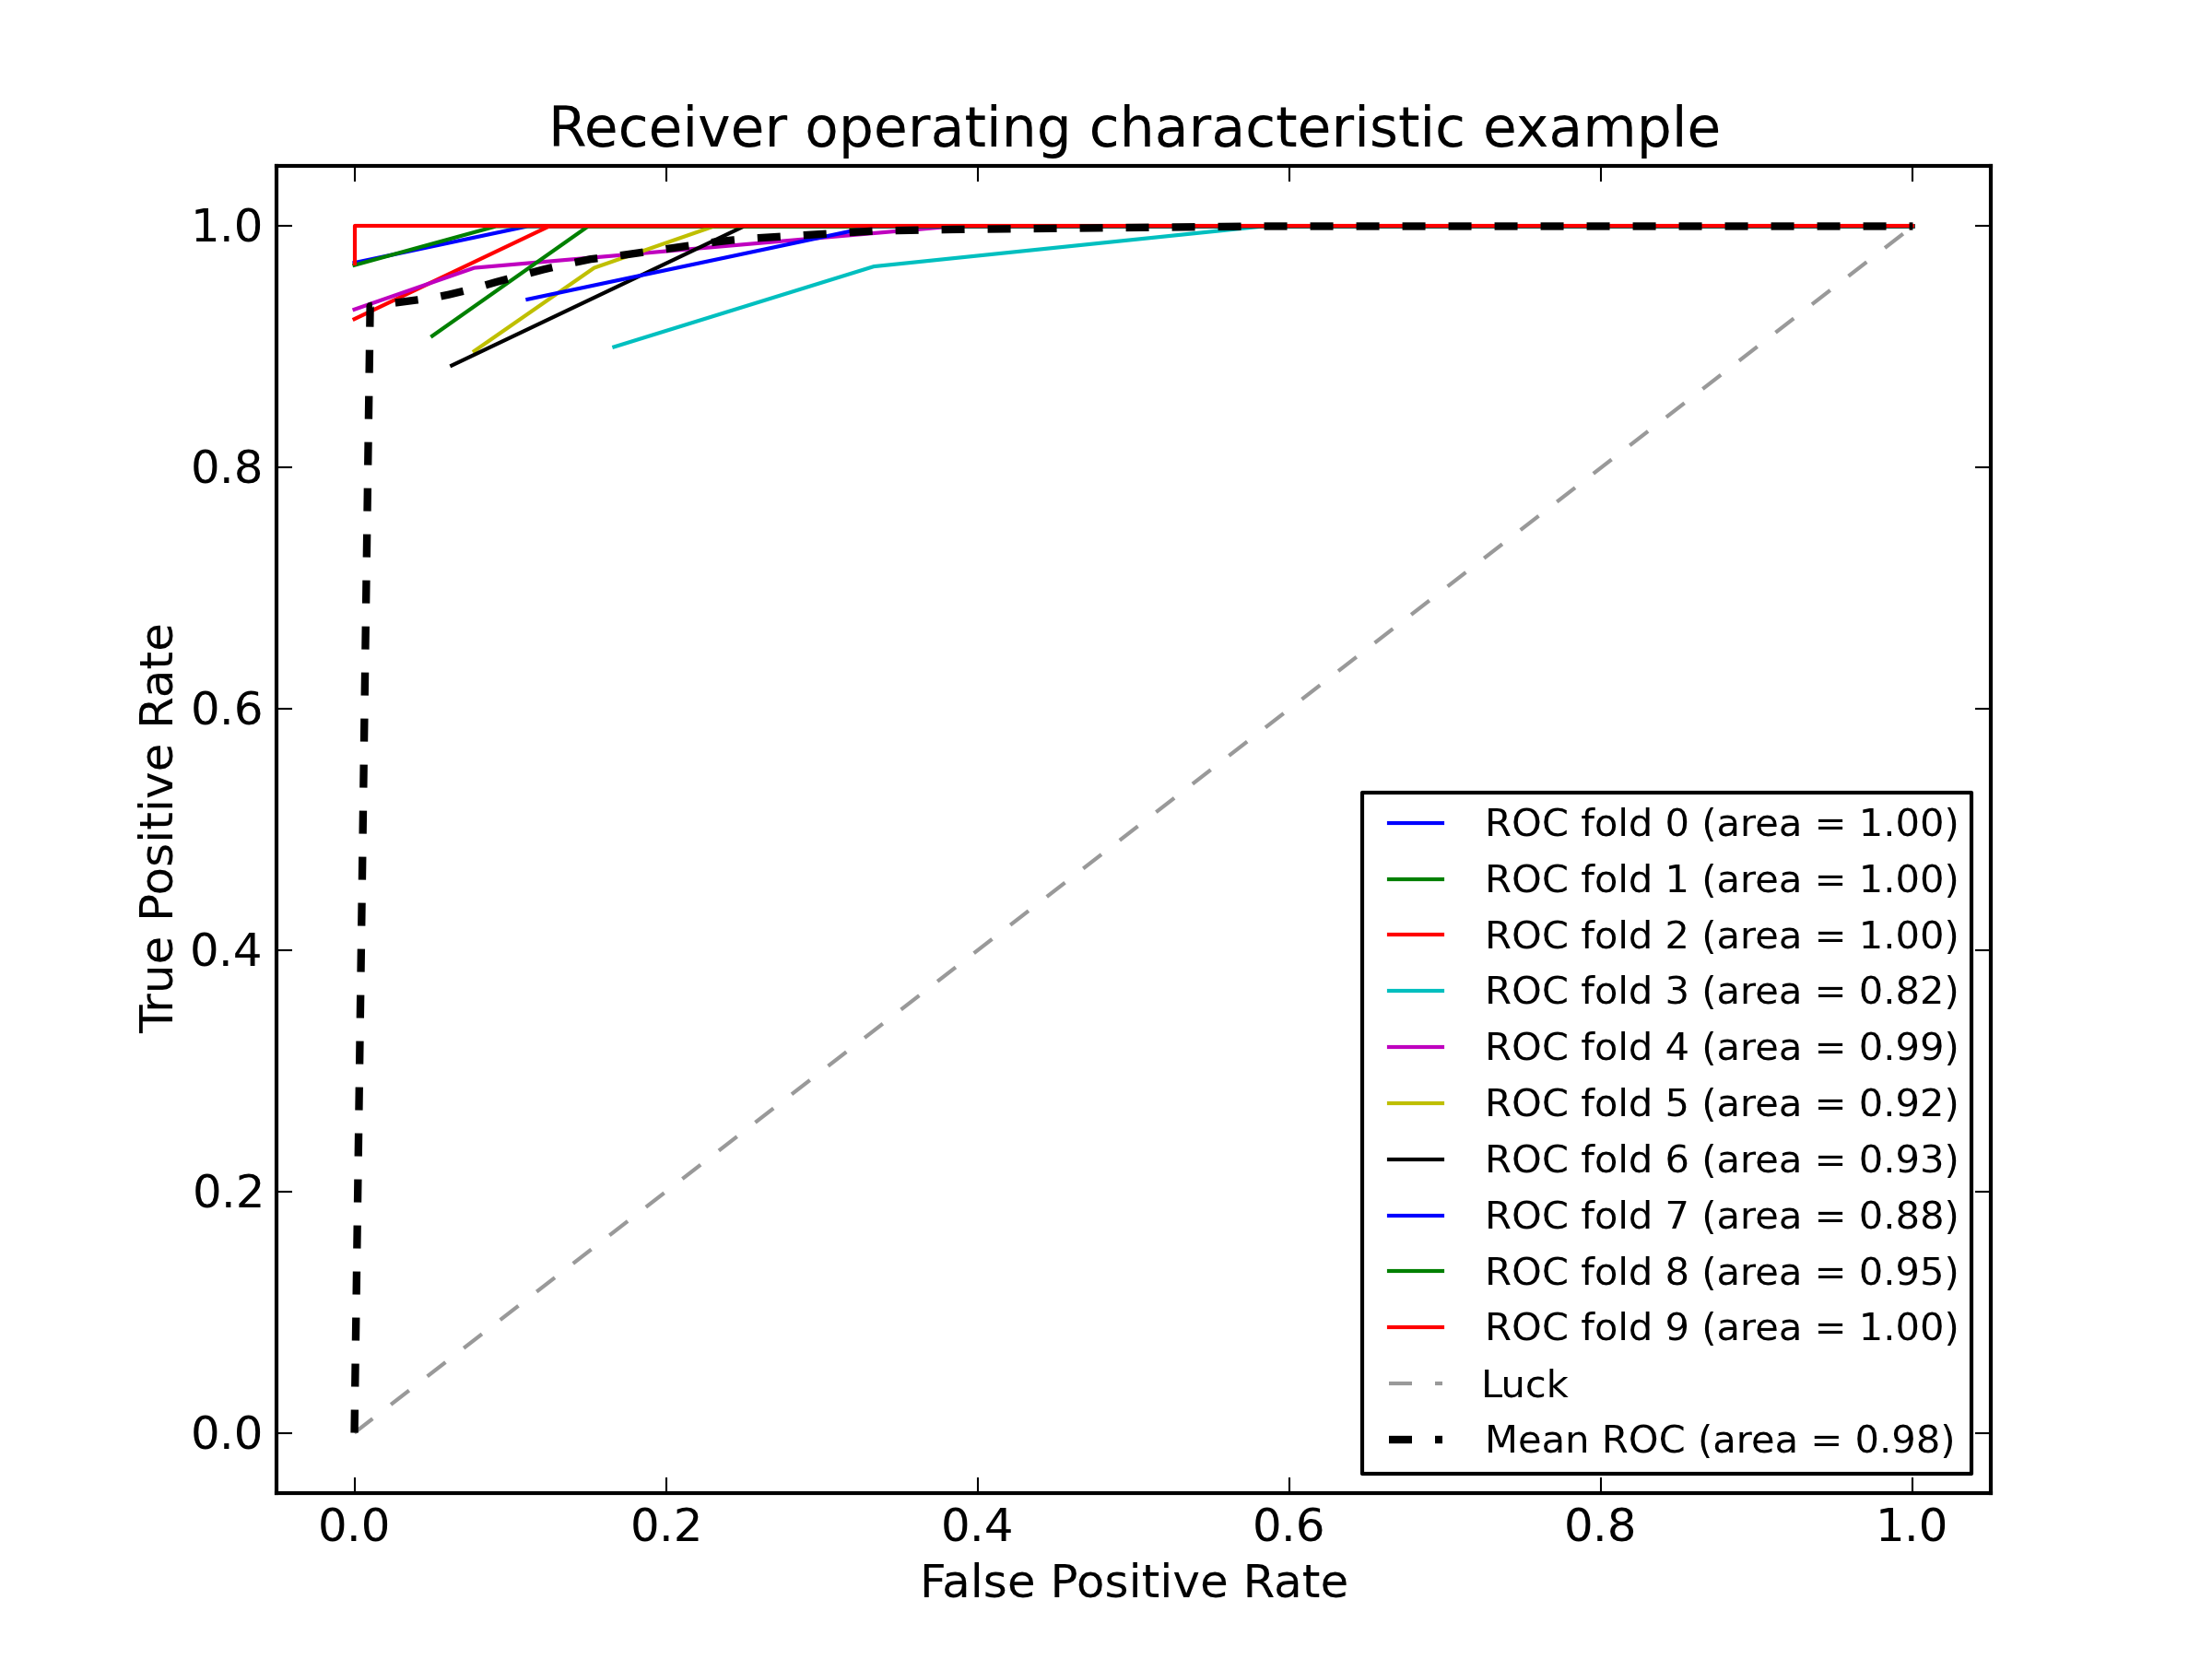
\includegraphics[width=0.36\textwidth]{pics/2_590_wmm.png}}
\quad
\subfloat[Stacking - Multi-Response Linear Models]{
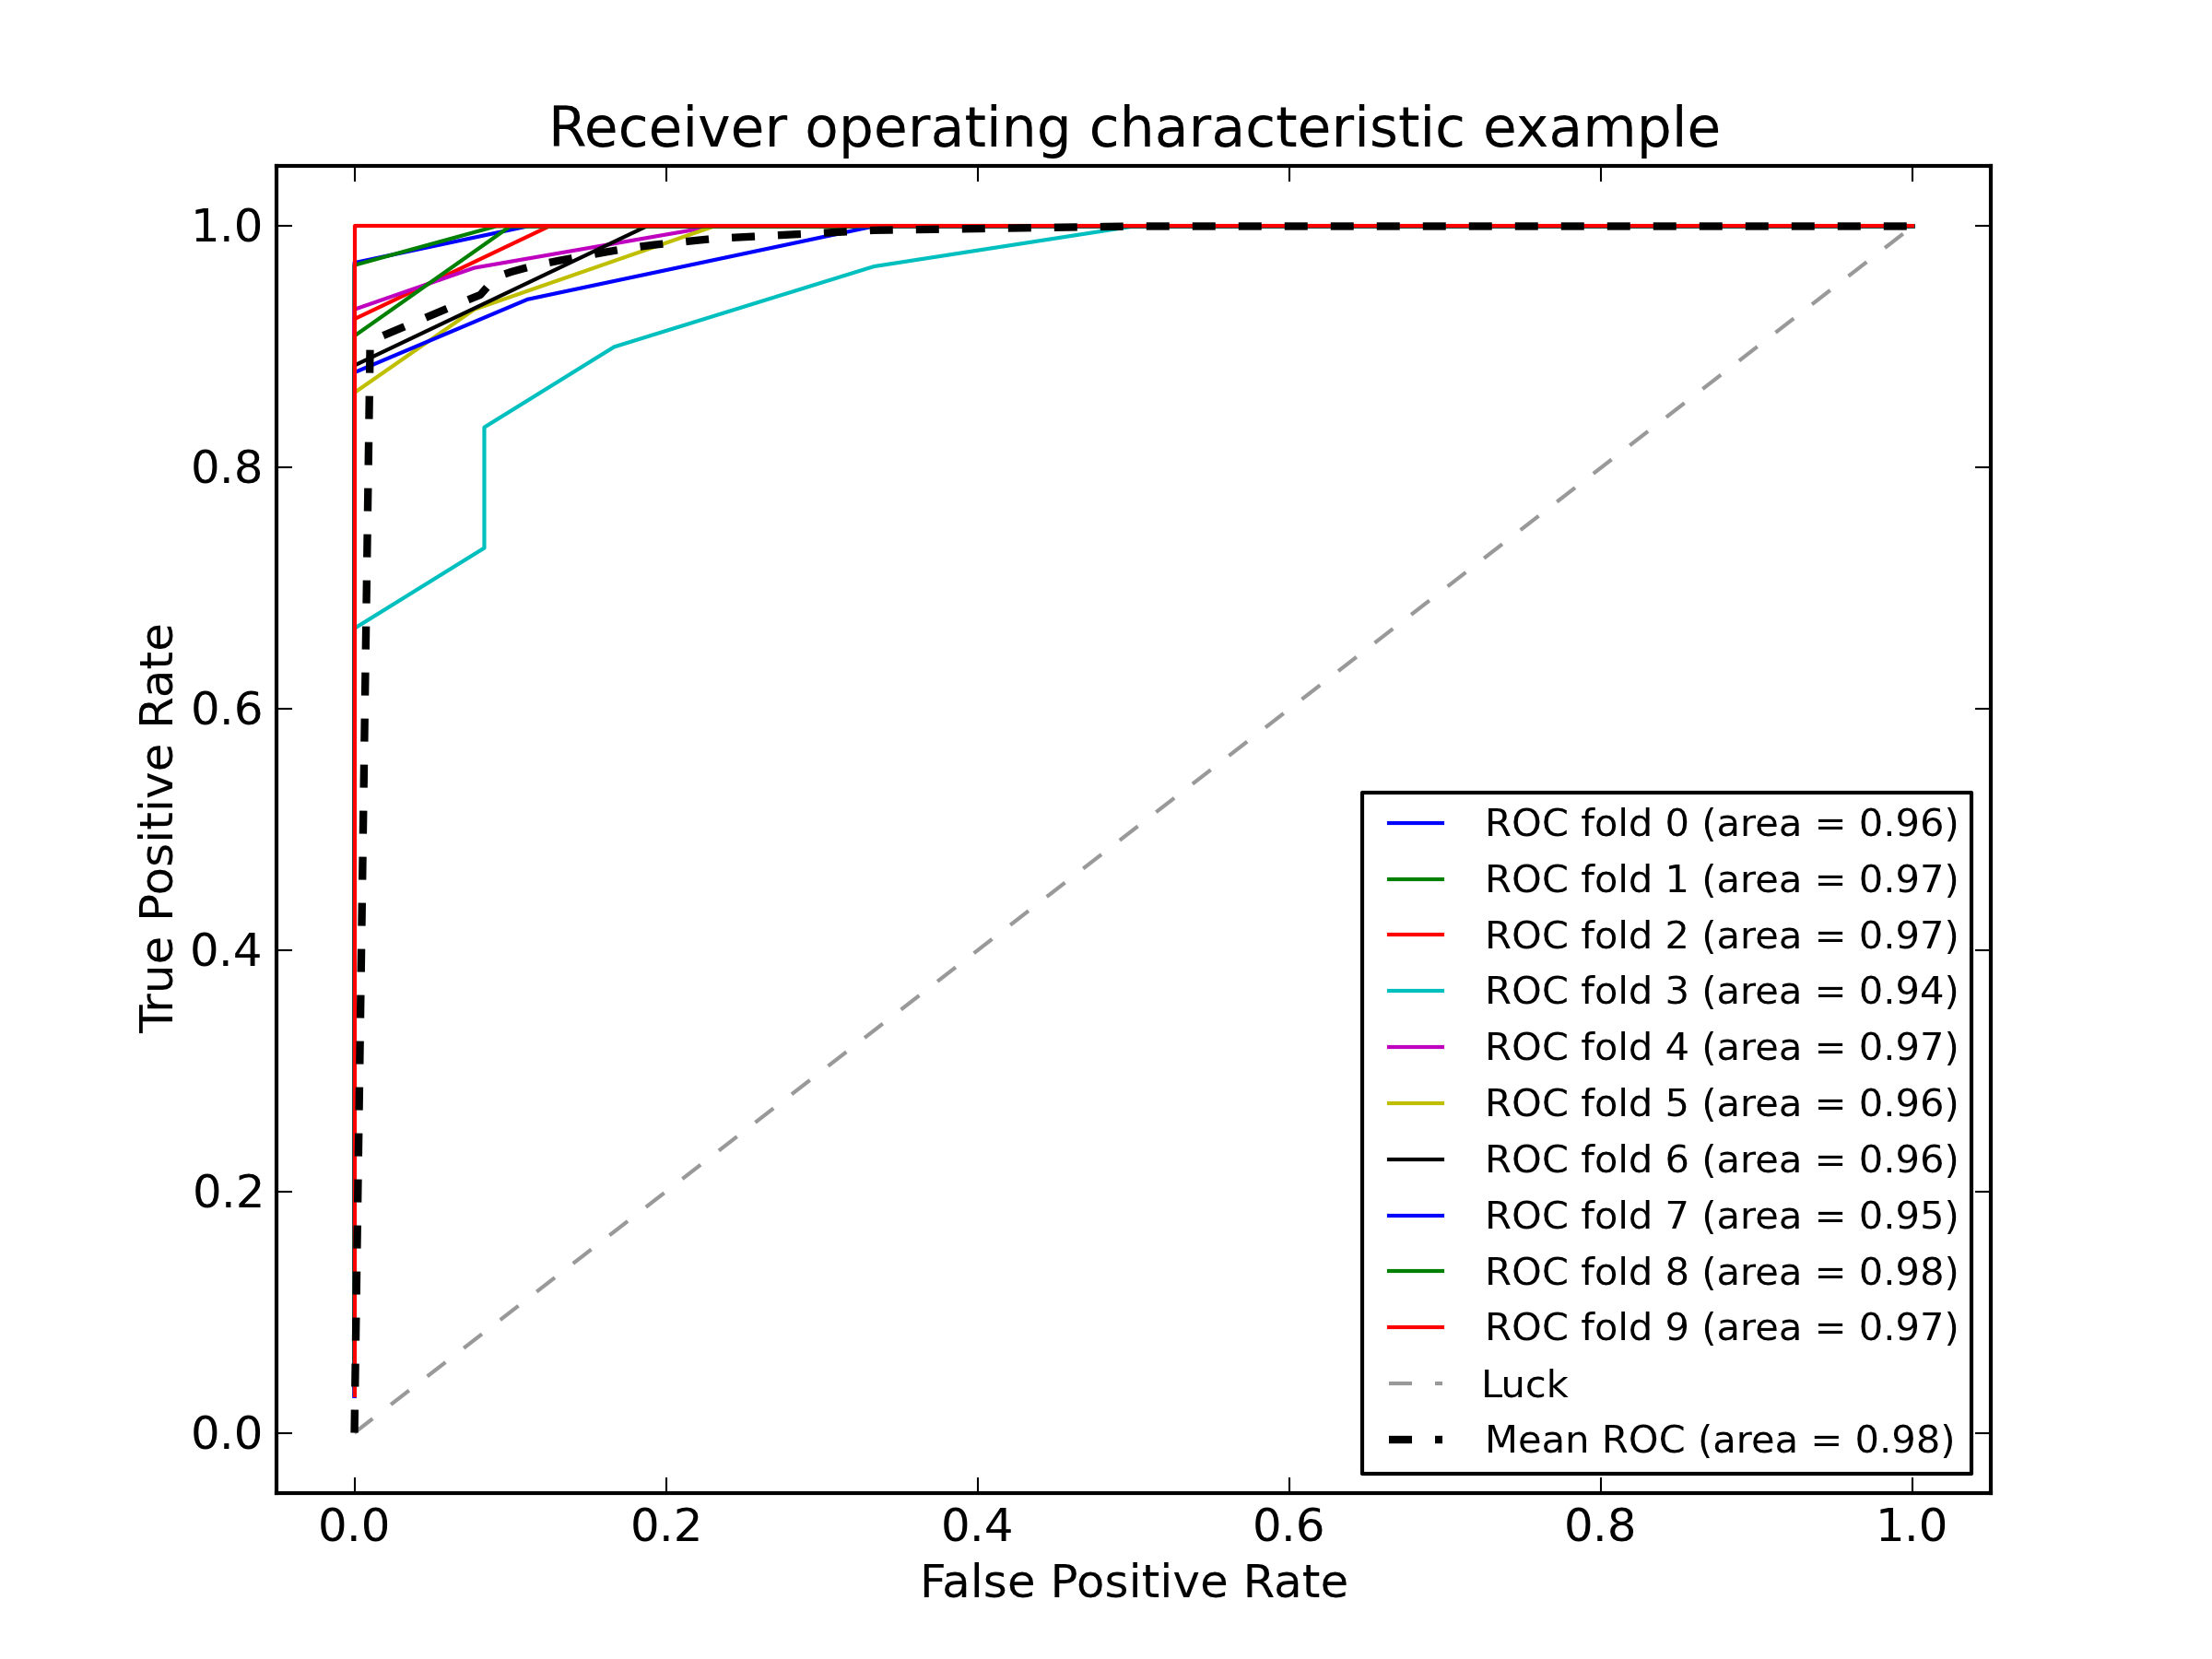
\includegraphics[width=0.36\textwidth]{pics/2_590_smm.png}}
\caption{Results for Features 1-9}
\label{fig:fig3}
\end{figure}